\chapter{Experiments and Evaluation}\label{ch:experiments}

This chapter evaluates attribution from split-streams and game-based backward routing through localization, faithfulness, robustness, and computational cost. It brings together the two papers' experiments and additional controls for numerical accuracy, perturbation protocols, and attribution-map sharpening.

\section{Experimental Setup}\label{sec:experimental_setup}\label{sec:quantus_evaluation}

We benchmark split methods on VGG-16~\parencite{Simonyan2015} and ResNet-18~\parencite{He2016resnet}, and game methods on VGG-16, ResNet-50 and ViT-B/16~\parencite{Dosovitskiy2021vit}, using PyTorch~\parencite{Paszke2019PyTorch} and torchvision ImageNet-1K checkpoints~\parencite{Deng2009,Russakovsky2015ilsvrc}\footnote{Checkpoint documentation: \url{https://docs.pytorch.org/vision/stable/models.html}; identifiers: Section~\ref{app:extended_protocol}.}. Attribution methods are described in Sections~\ref{sec:split_attribution_concept} and~\ref{sec:risk_aversion_regularization}; Appendix~\ref{app:baselines} describes the baselines and their implementations, and Section~\ref{ptnb:app:config-symbols} defines the game-mode parameters.

We tune the split-method attribution layers and formulas on a custom validation set of 50 ImageNet-S~\parencite{gao2022luss} images, one per class. We then evaluate the selected configurations on the disjoint 566-image test set, which supplies all reported split-method benchmark scores. Images use a resolution of $224\times224$. Explanations target the predicted class, including for misclassified images; localization uses the annotated object mask. Baselines use Captum, Zennit for $\gamma$-LRP, and separate Grad-CAM++ and LayerCAM implementations. Each method retains localization-selected and Pixel-Flipping-selected configurations (full settings and results: Section~\ref{app:saliency}).

The game methods and their baselines use 50 validation and 565 disjoint test images from ImageNet-S at the same resolution, with annotated-class targets. Pascal VOC 2012~\parencite{Everingham2010voc} tests cross-dataset transfer. The data filters and pixel-mask protocol are specified in Section~\ref{ptnb:app:protocol}.

Quantus~\parencite{Hedstrom2023} measures localization through Attribution Localization (AL), Pointing Game (PG) and Top-$k$ Intersection (TK), all $\uparrow$; faithfulness through Pixel Flipping (PF) and Selectivity (Sel; $\downarrow$); and robustness through Maximum and Average Sensitivity (MaxS, AvgS; $\downarrow$). Section~\ref{app:metrics} defines these metrics. The split tables report Pixel Flipping as score-drop AUC (PF$^{\mathrm{drop}}_5$, PF$^{\mathrm{drop}}_{20}$; $\uparrow$), perturbing 112 scalar input features per step, and Maximum Sensitivity with 25 random perturbations per image. The game campaign reports remaining-logit AUC (PF$_5$, PF$_{20}$; $\downarrow$), with 1,568 scalar features per step, and sensitivity with 50 perturbations on a common 200-image test subset. Both Pixel-Flipping implementations broadcast spatial attribution over color channels, indexing the flattened $C\times H\times W$ input: $150{,}528$ features for RGB images at this resolution.

Method abbreviations (Section~\ref{subsec:visual_attribution_related}) are GCAM (Grad-CAM), GCAM++ (Grad-CAM++), LCAM (LayerCAM), IntGrad (Integrated Gradients), SmGrad (SmoothGrad), and Guided GCAM (Guided Grad-CAM). Dark blue shading and bold type mark the best values within each caption's comparison; n/r means unreported in the source paper, and n/a means inapplicable.

\section{Split Methods: VGG-16}\label{sec:results_vgg}

\def\colA{0.10}
\def\colB{0.105}
\def\colSpace{0.0015\linewidth}

\begin{figure}[t]
\QualitativeImageContent{
    \centering

    \begin{minipage}[c]{\colA\linewidth}\centering\scriptsize\textbf{Class}\end{minipage}\hspace{\colSpace}%
    \begin{minipage}[c]{\colB\linewidth}\centering\scriptsize\textbf{Original}\end{minipage}\hspace{\colSpace}%
    \begin{minipage}[c]{\colB\linewidth}\centering\scriptsize\textbf{SplitLRP}\\\scriptsize\textbf{$R^{(10,\text{pos})}$ abs}\end{minipage}\hspace{\colSpace}%
    \begin{minipage}[c]{\colB\linewidth}\centering\scriptsize\textbf{LRP $\gamma$=0.25}\\\scriptsize\textbf{layer 5 abs}\end{minipage}\hspace{\colSpace}%
    \begin{minipage}[c]{\colB\linewidth}\centering\scriptsize\textbf{SplitCAM}\\\scriptsize\textbf{$\alpha=0.4$}\\\scriptsize\textbf{$\delta^{(14,g)}$}\end{minipage}\hspace{\colSpace}%
    \begin{minipage}[c]{\colB\linewidth}\centering\scriptsize\textbf{LayerCAM}\\\scriptsize\textbf{layer 14}\end{minipage}\hspace{\colSpace}%
    \begin{minipage}[c]{\colB\linewidth}\centering\scriptsize\textbf{SplitCAM}\\\scriptsize\textbf{$\alpha=0.3$}\\\scriptsize\textbf{$\delta^{(26,g)}$ abs}\end{minipage}\hspace{\colSpace}%
    \begin{minipage}[c]{\colB\linewidth}\centering\scriptsize\textbf{LayerCAM}\\\scriptsize\textbf{layer 26}\end{minipage}\hspace{\colSpace}%
    \begin{minipage}[c]{\colB\linewidth}\centering\scriptsize\textbf{SplitGrad}\\\scriptsize\textbf{$\alpha=0.3$}\\\scriptsize\textbf{$\delta^{(0,+,g)}$}\end{minipage}

    \vspace{0.25cm}

    \begin{minipage}[c]{\colA\linewidth}
        \centering
        \small goldfinch\\[1pt]
        {\scriptsize (0.9996)}
    \end{minipage}\hspace{\colSpace}%
    \begin{minipage}[c]{\colB\linewidth}
        \centering
        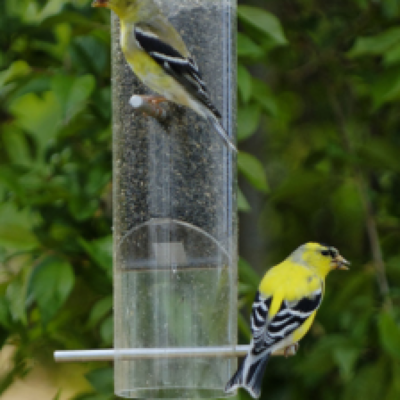
\includegraphics[width=\linewidth]{figures/experiments/saliency_quality/image_0030_ILSVRC2012_val_00030071.JPEG/original_image.png}
    \end{minipage}\hspace{\colSpace}%
    \begin{minipage}[c]{\colB\linewidth}
        \centering
        
\includegraphics[width=\linewidth]{figures/experiments/saliency_quality/image_0030_ILSVRC2012_val_00030071.JPEG/hybrid_lrp_scaling_max_winnerTakesItAllMaxpool_f10_cam_pp_abs.png}
    \end{minipage}\hspace{\colSpace}%
    \begin{minipage}[c]{\colB\linewidth}
        \centering
        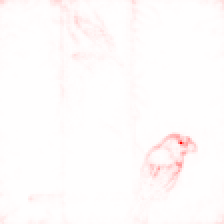
\includegraphics[width=\linewidth]{figures/experiments/saliency_quality/image_0030_ILSVRC2012_val_00030071.JPEG/zennit_lrp_gamma0.25_features_5_abs.png}
    \end{minipage}\hspace{\colSpace}%
    \begin{minipage}[c]{\colB\linewidth}
        \centering
        
\includegraphics[width=\linewidth]{figures/experiments/saliency_quality/image_0030_ILSVRC2012_val_00030071.JPEG/hybrid_cam_shift_40_scale_max_winnerTakesItAllMaxpool_f14_cam_g.png}
    \end{minipage}\hspace{\colSpace}%
    \begin{minipage}[c]{\colB\linewidth}
        \centering
        
\includegraphics[width=\linewidth]{figures/experiments/saliency_quality/image_0030_ILSVRC2012_val_00030071.JPEG/layer_cam_features_14_relu.png}
    \end{minipage}\hspace{\colSpace}%
    \begin{minipage}[c]{\colB\linewidth}
        \centering
        
\includegraphics[width=\linewidth]{figures/experiments/saliency_quality/image_0030_ILSVRC2012_val_00030071.JPEG/hybrid_cam_shift_30_scale_max_winnerTakesItAllMaxpool_f26_cam_g_abs.png}
    \end{minipage}\hspace{\colSpace}%
    \begin{minipage}[c]{\colB\linewidth}
        \centering
        
\includegraphics[width=\linewidth]{figures/experiments/saliency_quality/image_0030_ILSVRC2012_val_00030071.JPEG/layer_cam_features_26_relu.png}
    \end{minipage}\hspace{\colSpace}%
    \begin{minipage}[c]{\colB\linewidth}
        \centering
        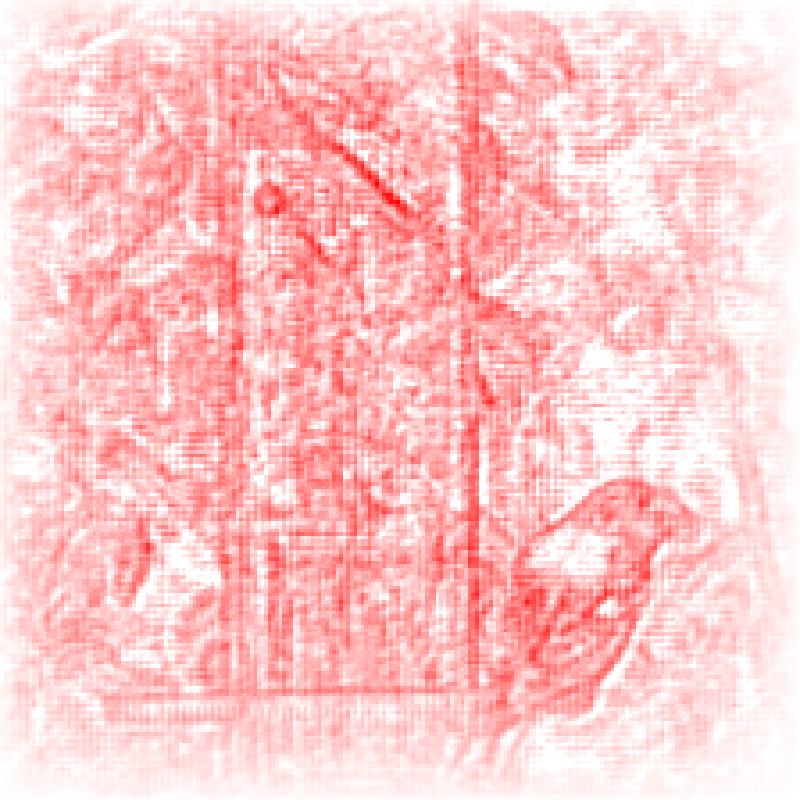
\includegraphics[width=\linewidth]{figures/experiments/saliency_quality/image_0030_ILSVRC2012_val_00030071.JPEG/hybrid_grad_shift_30_max_winnerTakesItAllMaxpool_f0_grad_pp.png}
    \end{minipage}%

    \vspace{0.25cm}

    \begin{minipage}[c]{\colA\linewidth}
        \centering
        \small sulphur butterfly\\[1pt]
        {\scriptsize (0.9999)}
    \end{minipage}\hspace{\colSpace}%
    \begin{minipage}[c]{\colB\linewidth}
        \centering
        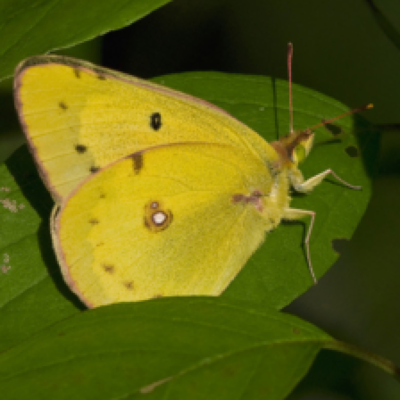
\includegraphics[width=\linewidth]{figures/experiments/saliency_quality/image_0106_ILSVRC2012_val_00019900.JPEG/original_image.png}
    \end{minipage}\hspace{\colSpace}%
    \begin{minipage}[c]{\colB\linewidth}
        \centering
        
\includegraphics[width=\linewidth]{figures/experiments/saliency_quality/image_0106_ILSVRC2012_val_00019900.JPEG/hybrid_lrp_scaling_max_winnerTakesItAllMaxpool_f10_cam_pp_abs.png}
    \end{minipage}\hspace{\colSpace}%
    \begin{minipage}[c]{\colB\linewidth}
        \centering
        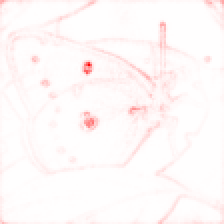
\includegraphics[width=\linewidth]{figures/experiments/saliency_quality/image_0106_ILSVRC2012_val_00019900.JPEG/zennit_lrp_gamma0.25_features_5_abs.png}
    \end{minipage}\hspace{\colSpace}%
    \begin{minipage}[c]{\colB\linewidth}
        \centering
        
\includegraphics[width=\linewidth]{figures/experiments/saliency_quality/image_0106_ILSVRC2012_val_00019900.JPEG/hybrid_cam_shift_40_scale_max_winnerTakesItAllMaxpool_f14_cam_g.png}
    \end{minipage}\hspace{\colSpace}%
    \begin{minipage}[c]{\colB\linewidth}
        \centering
        
\includegraphics[width=\linewidth]{figures/experiments/saliency_quality/image_0106_ILSVRC2012_val_00019900.JPEG/layer_cam_features_14_relu.png}
    \end{minipage}\hspace{\colSpace}%
    \begin{minipage}[c]{\colB\linewidth}
        \centering
        
\includegraphics[width=\linewidth]{figures/experiments/saliency_quality/image_0106_ILSVRC2012_val_00019900.JPEG/hybrid_cam_shift_30_scale_max_winnerTakesItAllMaxpool_f26_cam_g_abs.png}
    \end{minipage}\hspace{\colSpace}%
    \begin{minipage}[c]{\colB\linewidth}
        \centering
        
\includegraphics[width=\linewidth]{figures/experiments/saliency_quality/image_0106_ILSVRC2012_val_00019900.JPEG/layer_cam_features_26_relu.png}
    \end{minipage}\hspace{\colSpace}%
    \begin{minipage}[c]{\colB\linewidth}
        \centering
        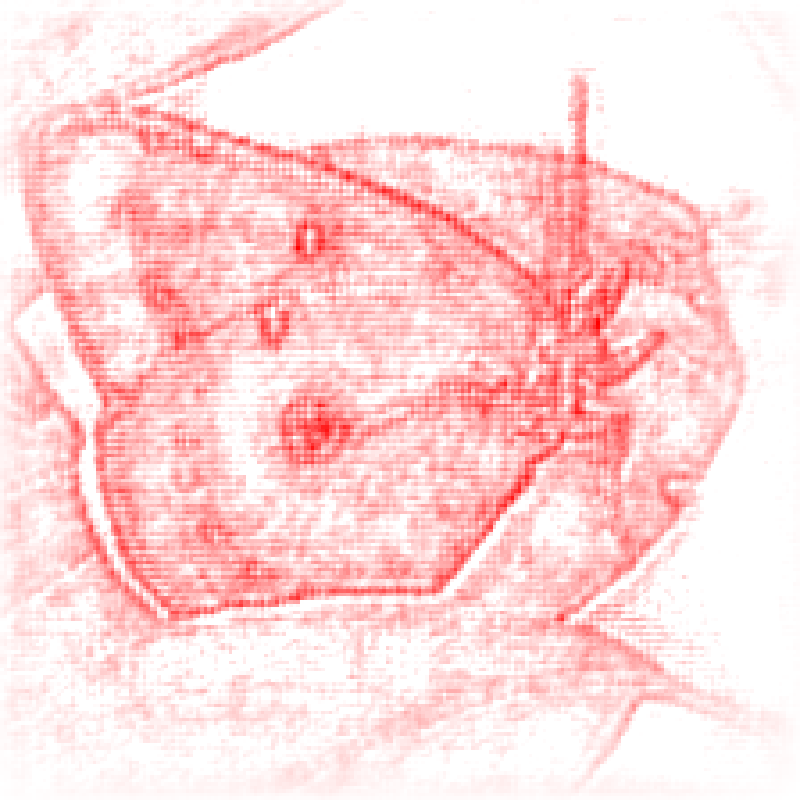
\includegraphics[width=\linewidth]{figures/experiments/saliency_quality/image_0106_ILSVRC2012_val_00019900.JPEG/hybrid_grad_shift_30_max_winnerTakesItAllMaxpool_f0_grad_pp.png}
    \end{minipage}%

    \vspace{0.25cm}

    \begin{minipage}[c]{\colA\linewidth}
        \centering
        \small goldfish\\[1pt]
        {\scriptsize (1.0000)}
    \end{minipage}\hspace{\colSpace}%
    \begin{minipage}[c]{\colB\linewidth}
        \centering
        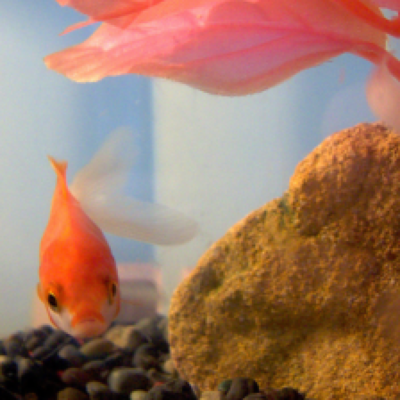
\includegraphics[width=\linewidth]{figures/experiments/saliency_quality/image_0005_ILSVRC2012_val_00020785.JPEG/original_image.png}
    \end{minipage}\hspace{\colSpace}%
    \begin{minipage}[c]{\colB\linewidth}
        \centering
        
\includegraphics[width=\linewidth]{figures/experiments/saliency_quality/image_0005_ILSVRC2012_val_00020785.JPEG/hybrid_lrp_scaling_max_winnerTakesItAllMaxpool_f10_cam_pp_abs.png}
    \end{minipage}\hspace{\colSpace}%
    \begin{minipage}[c]{\colB\linewidth}
        \centering
        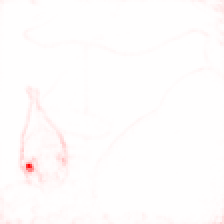
\includegraphics[width=\linewidth]{figures/experiments/saliency_quality/image_0005_ILSVRC2012_val_00020785.JPEG/zennit_lrp_gamma0.25_features_5_abs.png}
    \end{minipage}\hspace{\colSpace}%
    \begin{minipage}[c]{\colB\linewidth}
        \centering
        
\includegraphics[width=\linewidth]{figures/experiments/saliency_quality/image_0005_ILSVRC2012_val_00020785.JPEG/hybrid_cam_shift_40_scale_max_winnerTakesItAllMaxpool_f14_cam_g.png}
    \end{minipage}\hspace{\colSpace}%
    \begin{minipage}[c]{\colB\linewidth}
        \centering
        
\includegraphics[width=\linewidth]{figures/experiments/saliency_quality/image_0005_ILSVRC2012_val_00020785.JPEG/layer_cam_features_14_relu.png}
    \end{minipage}\hspace{\colSpace}%
    \begin{minipage}[c]{\colB\linewidth}
        \centering
        
\includegraphics[width=\linewidth]{figures/experiments/saliency_quality/image_0005_ILSVRC2012_val_00020785.JPEG/hybrid_cam_shift_30_scale_max_winnerTakesItAllMaxpool_f26_cam_g_abs.png}
    \end{minipage}\hspace{\colSpace}%
    \begin{minipage}[c]{\colB\linewidth}
        \centering
        
\includegraphics[width=\linewidth]{figures/experiments/saliency_quality/image_0005_ILSVRC2012_val_00020785.JPEG/layer_cam_features_26_relu.png}
    \end{minipage}\hspace{\colSpace}%
    \begin{minipage}[c]{\colB\linewidth}
        \centering
        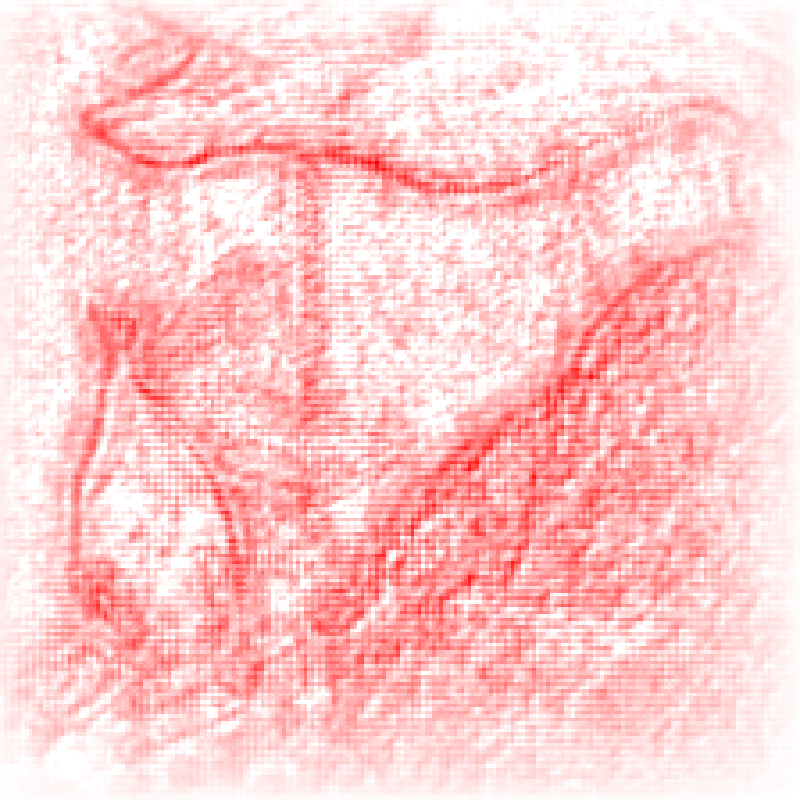
\includegraphics[width=\linewidth]{figures/experiments/saliency_quality/image_0005_ILSVRC2012_val_00020785.JPEG/hybrid_grad_shift_30_max_winnerTakesItAllMaxpool_f0_grad_pp.png}
    \end{minipage}%

    }%
\caption[VGG-16 saliency map comparison]{Saliency map comparison for VGG-16 on our custom ImageNet-S test split. Each row shows the predicted class (with confidence), original image, and saliency maps from different methods. Here $\alpha$ controls backward shifting and $\delta$ denotes shifted split-stream sensitivities (Section~\ref{subsec:backward_stabilization}); $R$ denotes SplitLRP relevance (Section~\ref{sec:split_lrp}).}
    \label{fig:vgg_saliency_comparison_main}
\end{figure}


\paragraph{Qualitative analysis.}
Figure~\ref{fig:vgg_saliency_comparison_main} qualitatively compares saliency maps from our split methods with their baseline counterparts at the best-performing layers. Mid-layer SplitCAM shares key visual characteristics with classical $\gamma$-\ac{lrp} from earlier layers. Compared to standard LayerCAM on the same layer it assigns more weight to object pixels, while still marking the key object features as especially important. For $\alpha \ll 0.5$, SplitGrad yields less focused yet finely aligned gradients that closely follow image details. We attribute this to the Maxout activation retaining preactivation information, unlike ReLU, which discards it in inactive neurons. Overall, mid-layer SplitCAM offers an effective balance between interpretability and focus (low entropy).

% Source: hiddenMonotonicity (Paper 1), sections/table_main_generated_vgg.tex — numbers verbatim.
\begin{table}[htb!]
    \centering
    \small
    \caption[Selected interpretability evaluation configurations: VGG-16]{Selected interpretability evaluation configurations (VGG-16, ImageNet-S test split). The \emph{wta} abbreviation indicates the use of the ``winner-take-all'' max-pooling implementation; \emph{sc} emphasizes the scaling procedure in the forward pass (Section~\ref{sec:stabilization_dc}). Within each block, the best value of each metric is bold with dark blue shading; AL of rows with Abs = n averages signed maps over method-dependent image subsets (Section~\ref{sec:experimental_setup}); the full comparison is in Table~\ref{tab:xai_eval_comprehensive_vgg}. The bracket notation in the layer column follows the upper indices of the split methods as introduced in Section~\ref{sec:split_attribution_concept}.}
    \label{tab:eval_vgg_main}
\TableContent{
    \begin{tabular}{p{4cm}cc cccccc}
        \toprule
    Method & Layer & Abs & Sel$\downarrow$ & AL$\uparrow$ & PG$\uparrow$ & PF$^{\mathrm{drop}}_5$$\uparrow$ & PF$^{\mathrm{drop}}_{20}$$\uparrow$ & MaxS$\downarrow$ \\
        \midrule
        \multicolumn{9}{c}{\textit{Split Methods}} \\
        \midrule
        SplitCAM (sc, $\alpha = 0.4$) & (12, g) & n & 4.720 & \cellbest{\textbf{0.651}} & 0.912 & 0.213 & 1.794 & 0.389 \\
        SplitCAM (sc, $\alpha = 0.4$) & (14, g) & n & \cellbest{\textbf{2.727}} & 0.563 & 0.836 & \cellbest{\textbf{0.300}} & \cellbest{\textbf{2.404}} & 1.012 \\
        SplitCAM (sc, $\alpha = 0.4$, wta) & (26, +, g) & y & 4.711 & 0.635 & \cellbest{\textbf{0.938}} & 0.165 & 1.590 & 0.456 \\
        SplitGrad ($\alpha = 0.4$, wta) & (12, +, g) & n & 4.735 & 0.635 & 0.883 & 0.186 & 1.756 & 0.651 \\
        SplitGrad ($\alpha = 0.4$, wta) & (14, +, g) & y & 3.287 & 0.540 & 0.818 & 0.249 & 2.186 & 0.857 \\
        SplitLRP (sc, wta) & (26, pos) & y & 5.168 & 0.588 & 0.871 & 0.151 & 1.473 & \cellbest{\textbf{0.282}} \\
        \midrule
        \multicolumn{9}{c}{\textit{Baselines (With Layer Optimization)}} \\
        \midrule
        Guided Backprop & 2 & n & 3.276 & \cellbest{\textbf{0.632}} & 0.883 & 0.281 & 2.302 & 0.571 \\
        Guided Backprop & 5 & n & 3.448 & 0.614 & \cellbest{\textbf{0.887}} & 0.240 & 2.091 & \cellbest{\textbf{0.375}} \\
        LCAM & 14 & n/a & \cellbest{\textbf{2.792}} & 0.576 & 0.798 & \cellbest{\textbf{0.317}} & \cellbest{\textbf{2.474}} & 2.656 \\
        LCAM & 2 & n/a & 3.128 & 0.580 & 0.855 & 0.300 & 2.191 & 5.508 \\
        LRP $\gamma=0.25$ & 0 & n & 3.189 & 0.615 & 0.680 & 0.218 & 1.918 & 0.519 \\
        LRP $\gamma=0.25$ & 14 & n & 3.593 & 0.577 & 0.611 & 0.279 & 2.255 & 0.491 \\
        \midrule
        \multicolumn{9}{c}{\textit{Baselines}} \\
        \midrule
        DeepLIFT & 0 & y & 4.447 & 0.551 & 0.726 & \cellbest{\textbf{0.281}} & \cellbest{\textbf{1.945}} & 1.053 \\
        Feature Ablation & 0 & y & 6.029 & 0.479 & 0.624 & 0.123 & 1.250 & 0.859 \\
        GradientSHAP & 0 & y & 4.808 & 0.552 & 0.783 & 0.261 & 1.862 & 1.142 \\
        GCAM++ & 30 & n & 5.955 & \cellbest{\textbf{0.564}} & \cellbest{\textbf{0.827}} & 0.130 & 1.245 & \cellbest{\textbf{0.401}} \\
        IntGrad & 0 & y & 4.838 & 0.554 & 0.797 & 0.262 & 1.851 & 1.069 \\
        Occlusion & 0 & y & 5.214 & 0.499 & 0.716 & 0.130 & 1.217 & 0.699 \\
        Random Baseline & 0 & y & \cellbest{\textbf{3.570}} & 0.425 & 0.458 & 0.203 & 1.585 & n/r \\
        \bottomrule
    \end{tabular}
}%
\end{table}


\paragraph{Quantitative analysis.}
Tables~\ref{tab:eval_vgg_main} and~\ref{tab:eval_res_main} compare selected attribution configurations on VGG-16 and ResNet-18 across Quantus metrics. The \emph{Abs} column specifies whether absolute saliency values were used prior to evaluation in Quantus. Full comparisons, including all reported layers and configurations, are in Tables~\ref{tab:xai_eval_comprehensive_vgg} and~\ref{tab:xai_eval_comprehensive_res} (Appendix~\ref{app:saliency}).

Overall, the considered backpropagation-based attribution methods heavily depend on the selected network layer; see Section~\ref{app:ablation} for extensive ablation.

On VGG-16, SplitCAM achieves strong localization and Selectivity results: Pointing Game $0.938$ versus Guided Backprop's $0.887$, Attribution Localization $0.651$ versus Guided Backprop's $0.632$, and Selectivity $2.727$ versus LayerCAM's $2.792$, with the SplitCAM values drawn from different layers. LayerCAM has the highest displayed Pixel Flipping score-drop AUCs, $0.317$ and $2.474$, versus SplitCAM's $0.300$ and $2.404$. SplitLRP achieves the lowest Maximum Sensitivity, $0.282$, versus Guided Backprop's $0.375$, and improves Pointing Game over the displayed classical $\gamma$-\ac{lrp} configurations.

\section{Split Methods: ResNet-18}\label{sec:results_resnet}

% Source: hiddenMonotonicity (Paper 1), sections/table_main_generated_res.tex — numbers verbatim.
\begin{table}[htb!]
    \centering
    \small
    \caption[Selected interpretability evaluation configurations: ResNet-18]{Selected interpretability evaluation configurations (ResNet-18, ImageNet-S test split). Highlighting identifies the best values among the displayed rows; the full comparison is in Table~\ref{tab:xai_eval_comprehensive_res}. The triples $x.y.z$ are a ResNet-18-internal indexing of the convolutional layer at which the attribution maps are calculated. See the caption of Table~\ref{tab:eval_vgg_main} for further abbreviations and table explanation.}
    \label{tab:eval_res_main}
\TableContent{
    \resizebox{\textwidth}{!}{%
    \begin{tabular}{p{4cm}cc cccccc}
        \toprule
    Method & Layer & Abs & Sel$\downarrow$ & AL$\uparrow$ & PG$\uparrow$ & PF$^{\mathrm{drop}}_5$$\uparrow$ & PF$^{\mathrm{drop}}_{20}$$\uparrow$ & MaxS$\downarrow$ \\
         \midrule
        \multicolumn{9}{c}{\textit{SplitCAM Methods}} \\
        \midrule
        SplitCAM (sc, $\alpha = 0.3$, wta) & (1.0.2, g) & n & \cellbest{\textbf{3.503}} & 0.487 & 0.747 & 0.168 & 1.395 & 1.277 \\
        SplitCAM (sc, $\alpha = 0.3$, wta) & (4.1.2, g) & n & 5.654 & 0.673 & \cellbest{\textbf{0.972}} & 0.081 & 0.880 & 0.233 \\
        SplitGrad ($\alpha = 0.3$, wta) & (1.0.2, g) & y & 4.449 & 0.513 & 0.777 & 0.149 & 1.266 & 0.813 \\
        SplitGrad ($\alpha = 0.3$, wta) & (4.1.2, g) & y & 5.663 & 0.649 & \cellbest{\textbf{0.972}} & 0.082 & 0.882 & 0.219 \\
        SplitLRP (sc, wta) & (conv1, pos) & y & 6.313 & 0.506 & 0.587 & 0.056 & 0.697 & 0.755 \\
        \midrule
        \multicolumn{9}{c}{\textit{Baselines (With Layer Optimization)}} \\
        \midrule
        Guided GCAM & 4.0.2 & n & 4.929 & \cellbest{\textbf{0.742}} & 0.866 & 0.119 & 1.008 & 0.687 \\
        GCAM & 4.1.2 & n & 6.070 & 0.554 & 0.945 & 0.076 & 0.829 & \cellbest{\textbf{0.131}} \\
        LCAM & 2.0.2 & n & 3.690 & 0.549 & 0.865 & 0.144 & 1.428 & 0.913 \\
        LCAM & 4.1.1 & n & 5.661 & 0.664 & 0.971 & 0.083 & 0.890 & 0.227 \\
        LRP $\gamma=0.25$ & conv1 & y & 3.550 & 0.656 & 0.852 & \cellbest{\textbf{0.213}} & 1.737 & 0.521 \\
        \midrule
        \multicolumn{9}{c}{\textit{Baselines}} \\
        \midrule
        Guided Backprop & conv1 & n & 3.517 & 0.621 & 0.867 & 0.212 & \cellbest{\textbf{1.757}} & 0.459 \\
        GradientSHAP & conv1 & y & 5.269 & 0.527 & 0.779 & 0.166 & 1.227 & 1.074 \\
        IntGrad & conv1 & y & 5.265 & 0.528 & 0.777 & 0.167 & 1.226 & 0.994 \\
        Feature Ablation & conv1 & n & 4.655 & 0.136 & 0.684 & 0.188 & 1.388 & 1.077 \\
        Occlusion & conv1 & n & 5.300 & 0.179 & 0.726 & 0.130 & 1.030 & 0.785 \\
        Deconvolution & conv1 & n & 3.934 & 0.484 & 0.666 & 0.147 & 1.203 & 0.751 \\
        Random Baseline & n/a & y & 4.071 & 0.425 & 0.440 & 0.147 & 1.067 & n/r \\
        \bottomrule
    \end{tabular}
    }%
}%
\end{table}


On ResNet-18 (Table~\ref{tab:eval_res_main}), SplitCAM achieves the lowest reported Selectivity, $3.503$, compared with $3.517$ for Guided Backprop. SplitCAM and SplitGrad reach Pointing Game $0.972$ versus LayerCAM's $0.971$. SplitCAM's Attribution Localization is $0.673$ versus LayerCAM's $0.664$, while Guided Grad-CAM leads the full comparison at $0.742$ (Table~\ref{tab:xai_eval_comprehensive_res}).

\section{Split-Method Stabilization and Sanity Checks}\label{sec:ablations}

\paragraph{Backward stabilization.}\label{subsec:alpha_ablation}

Table~\ref{tab:alpha_ablation_main} presents the performance of one selected SplitGrad and one SplitCAM configuration across different shifting parameters $\alpha$, evaluated on our custom ImageNet-S test split. As explained in Section~\ref{sec:stabilization_dc}, $\alpha$ controls backward pass stabilization: $\alpha = 0$ means no stabilization and $\alpha = 0.5$ yields scaled original gradients (Theorem~\ref{thm:closed_formula_shift}). Reducing $\alpha$ from $0.5$ to $0.4$ improves both configurations' Pointing Game and Attribution Localization, while SplitCAM's PF$^{\mathrm{drop}}_{20}$ falls from $1.607$ to $1.585$. SplitGrad peaks in PF$^{\mathrm{drop}}_{20}$ at $\alpha = 0.4$ and localization at $\alpha = 0.35$; SplitCAM's Pointing Game and Attribution Localization peak at $0.4$ and $0.35$, respectively. \begin{changed}Overall, intermediate values $\alpha=0.35$--$0.45$ give the best localization and Pixel Flipping results in these configurations, while $\alpha=0$ minimizes Maximum Sensitivity.\end{changed} Section~\ref{app:ablation} (Table~\ref{tab:alpha_comparison_by_method}) gives the full grid and compares convex with winner-takes-it-all max-pooling.

% Source: hiddenMonotonicity (Paper 1), sections/alpha_ablation_main.tex — numbers verbatim, restyled to booktabs.
\begin{table}[htb]
    \centering
    \footnotesize
    \caption[Alpha comparison for SplitGrad and SplitCAM]{Comparison of different $\alpha$ parameters for one SplitGrad and one SplitCAM configuration, both in \emph{wta} and \emph{abs} mode, evaluated on the custom ImageNet-S test split.}
    \label{tab:alpha_ablation_main}
\TableContent{
    \begin{adjustbox}{max width=\linewidth}
\begin{tabular}{ll cccccc}
    \toprule
    \textbf{Method} & \textbf{Metric} & $\alpha \ .50$ & $\alpha \ .45$ & $\alpha \ .40$ & $\alpha \ .35$ & $\alpha \ .30$ & $\alpha \ .00$ \\
    \midrule
    \multirow{4}{*}{\begin{tabular}[c]{@{}l@{}}\textbf{SplitGrad}\\(26, g)\end{tabular}} & PG$\uparrow$ & 0.898 & 0.906 & 0.947 & \cellbest{\textbf{0.956}} & 0.889 & 0.401 \\
     & AL$\uparrow$ & 0.543 & 0.548 & 0.605 & \cellbest{\textbf{0.617}} & 0.535 & 0.449 \\
     & MaxS$\downarrow$ & 0.616 & 0.607 & 0.440 & 0.238 & 0.334 & \cellbest{\textbf{0.028}} \\
     & PF$^{\mathrm{drop}}_{20}$ $\uparrow$ & 1.527 & 1.534 & \cellbest{\textbf{1.581}} & 1.448 & 1.317 & 1.247 \\
    \midrule
    \multirow{4}{*}{\begin{tabular}[c]{@{}l@{}}\textbf{SplitCAM}\\(26, +, g)\end{tabular}} & PG$\uparrow$ & 0.868 & 0.868 & \cellbest{\textbf{0.938}} & 0.933 & 0.613 & 0.855 \\
     & AL$\uparrow$ & 0.550 & 0.554 & 0.635 & \cellbest{\textbf{0.663}} & 0.403 & 0.513 \\
     & MaxS$\downarrow$ & 0.691 & 0.682 & 0.457 & 0.265 & 0.251 & \cellbest{\textbf{0.120}} \\
     & PF$^{\mathrm{drop}}_{20}$ $\uparrow$ & 1.607 & \cellbest{\textbf{1.609}} & 1.585 & 1.499 & 0.853 & 1.507 \\
    \bottomrule
    \end{tabular}
\end{adjustbox}
}%
\end{table}


\paragraph{Forward stabilization.}
Without forward stabilization, late VGG-16 SplitCAM activations reach the order of $10^{18}$, with reconstruction errors of order $10^9$ despite per-layer correction. Section~\ref{app:forward_ablation} reports SplitCAM without forward stabilization and with shifting.

\paragraph{Randomization sanity checks.}
After randomizing VGG-16's last three fully connected layers, every reported SplitCAM and SplitGrad configuration has lower SSIM than every listed baseline, while HOG and Spearman comparisons are mixed (Section~\ref{app:p1_sanity}).

\paragraph{Runtime.}
SplitCAM takes $0.33$--$0.44$\,s per image; Table~\ref{tab:timing_comparison} gives the full runtime comparison and Section~\ref{app:p1_timing} its measurement scope.

\section{Directly Trained Difference-of-Convex Models on MNIST}\label{sec:dcinns}

To study mechanisms exposed by the \ac{dc} decomposition of pretrained networks (Sections~\ref{sec:split_cam}--\ref{sec:split_grad}), we directly train small DC input neural networks (DCINNs) and their monotone relatives on MNIST. Their shared opposing-stream structure provides a controlled setting for examining class-dependent sensitivities on present and candidate missing strokes.

\paragraph{Architecture and training.}\label{subsec:dcinn_architecture}

We use the \ac{icnn} and monotone-network definitions of Section~\ref{sec:convex_monotone_foundations}; only the \ac{icnn} leaves its first affine layer unconstrained.

The \textbf{DIC-model} (directly trained as the difference of two input-convex neural networks) denotes $g-h$ with both streams input-convex, while the \textbf{DM-model} (directly trained as the difference of two monotone networks) denotes $g-h$ with both streams monotone. For each base model we also evaluate the \emph{inverted-input} variant (DICIN / DMIN), where the $h$-stream processes $\1-x$, motivated by sensitivities to missing features.

Three implementation choices matter in practice.
\begin{itemize}
	\item \emph{Activations.} Both streams use convex, monotone rank-2 Maxout units~\parencite{Goodfellow2013Maxout}, which consistently outperformed \ac{relu} streams in the difference setting. Their constrained layers use the same non-negative-weight Maxout building blocks as the split-stream construction in Section~\ref{sec:dc_splitting_relu}.
	\item \emph{Non-negativity.} Constrained weights are parameterized as $p(\tilde{W})$ with free parameters $\tilde{W}$ and a positivity transform $p$; among softplus, exponential and squaring, $p = \relu$ with absolute-value-of-Gaussian initialization gave the best test accuracy. Positive initialization avoids inactive raw weights: for $\tilde w<0$, the ReLU transform has zero derivative and blocks the task-loss gradient to $\tilde w$. The transform is also applied to biases and to the scale and shift parameters of batch-normalization layers.
	\item \emph{Regularization.} To limit activation growth, we use small initial weights and weight decay, reported as $10^{-3}$ in \textcite{hiddenMono}.
\end{itemize}

We train two base architectures on MNIST: \texttt{cnn\_maxout}, a \ac{cnn} with four convolutional layers (32, 64, 128 and 128 channels with batch normalization) followed by three fully connected layers, roughly $1.2$ million parameters in total, and \texttt{mlp\_maxout}, a wide four-layer \ac{mlp} ($784 \to 800 \to 800 \to 800 \to 10$) with roughly $4.2$ million parameters --- each in eight variants: unconstrained (None), single-stream constrained (IC, Mon), and difference-of-two models (DIC, DM, DICIN, DMIN, and an unconstrained difference baseline, \texttt{Diff\_None}).

% Source: arxive/hiddenMonotonicity/appendix/table_model_accuracy.tex.
\begin{table}[htbp]
    \centering
    \caption[MNIST test accuracy across eight model variants]{MNIST test accuracy (\%) for all eight model variants~\parencite{hiddenMono}. Cells show median [minimum, maximum] over ten random seeds.}
    \label{tab:cdinn_acc}
\TableContent{
    \small
    \setlength{\tabcolsep}{5pt}
    \begin{tabular}{lcc}
        \toprule
        Variant & \texttt{mlp\_maxout} & \texttt{cnn\_maxout} \\
        \midrule
        IC & 98.36 {\scriptsize [98.07, 98.69]} & 99.16 {\scriptsize [98.86, 99.27]} \\
        Mon & 98.30 {\scriptsize [97.64, 98.49]} & 98.50 {\scriptsize [98.19, 98.79]} \\
        None & 98.39 {\scriptsize [98.07, 98.63]} & 99.19 {\scriptsize [98.61, 99.44]} \\
        DIC & 98.56 {\scriptsize [98.33, 98.96]} & 97.94 {\scriptsize [97.81, 98.04]} \\
        DM & 98.55 {\scriptsize [98.23, 98.71]} & 98.06 {\scriptsize [97.99, 98.19]} \\
        Diff\_None & 98.47 {\scriptsize [98.19, 98.72]} & 97.94 {\scriptsize [97.72, 98.45]} \\
        DICIN & 98.58 {\scriptsize [98.41, 98.84]} & 98.17 {\scriptsize [97.96, 98.34]} \\
        DMIN & 98.54 {\scriptsize [98.36, 98.65]} & 98.28 {\scriptsize [98.17, 98.54]} \\
        \bottomrule
    \end{tabular}
}%
\end{table}


\paragraph{Stream sensitivities and candidate counterfactual features.}\label{subsec:counterfactual_features}

For an inverted-input class logit $f(x)=g(x)-h(\1-x)$, the complete gradient at differentiable inputs is
\[
\nabla f(x)=\nabla g(x)+(\nabla h)(\1-x).
\]
The complement and subtraction cancel the two minus signs: a positive entry of $(\nabla h)(\1-x)$ (bright blue pixel) indicates positive local sensitivity of the contribution $-h(\1-x)$ to increasing the original input. The unconstrained first layer means that ICNN gradients need not be non-negative in the original input coordinates.

\begin{figure}[t]
\QualitativeImageContent{
	\centering
	\begin{minipage}[c]{0.15\linewidth}
		\centering
		
\includegraphics[width=\linewidth]{saliency/mnist_split_ic_saliency/image_030_true_3_pred_3/original.png}\\[-1pt]
		{\scriptsize Original}
	\end{minipage}\hspace{0.015\linewidth}%
	\begin{minipage}[c]{0.80\linewidth}
		\centering
		\begin{minipage}[b]{0.19\linewidth}\centering
			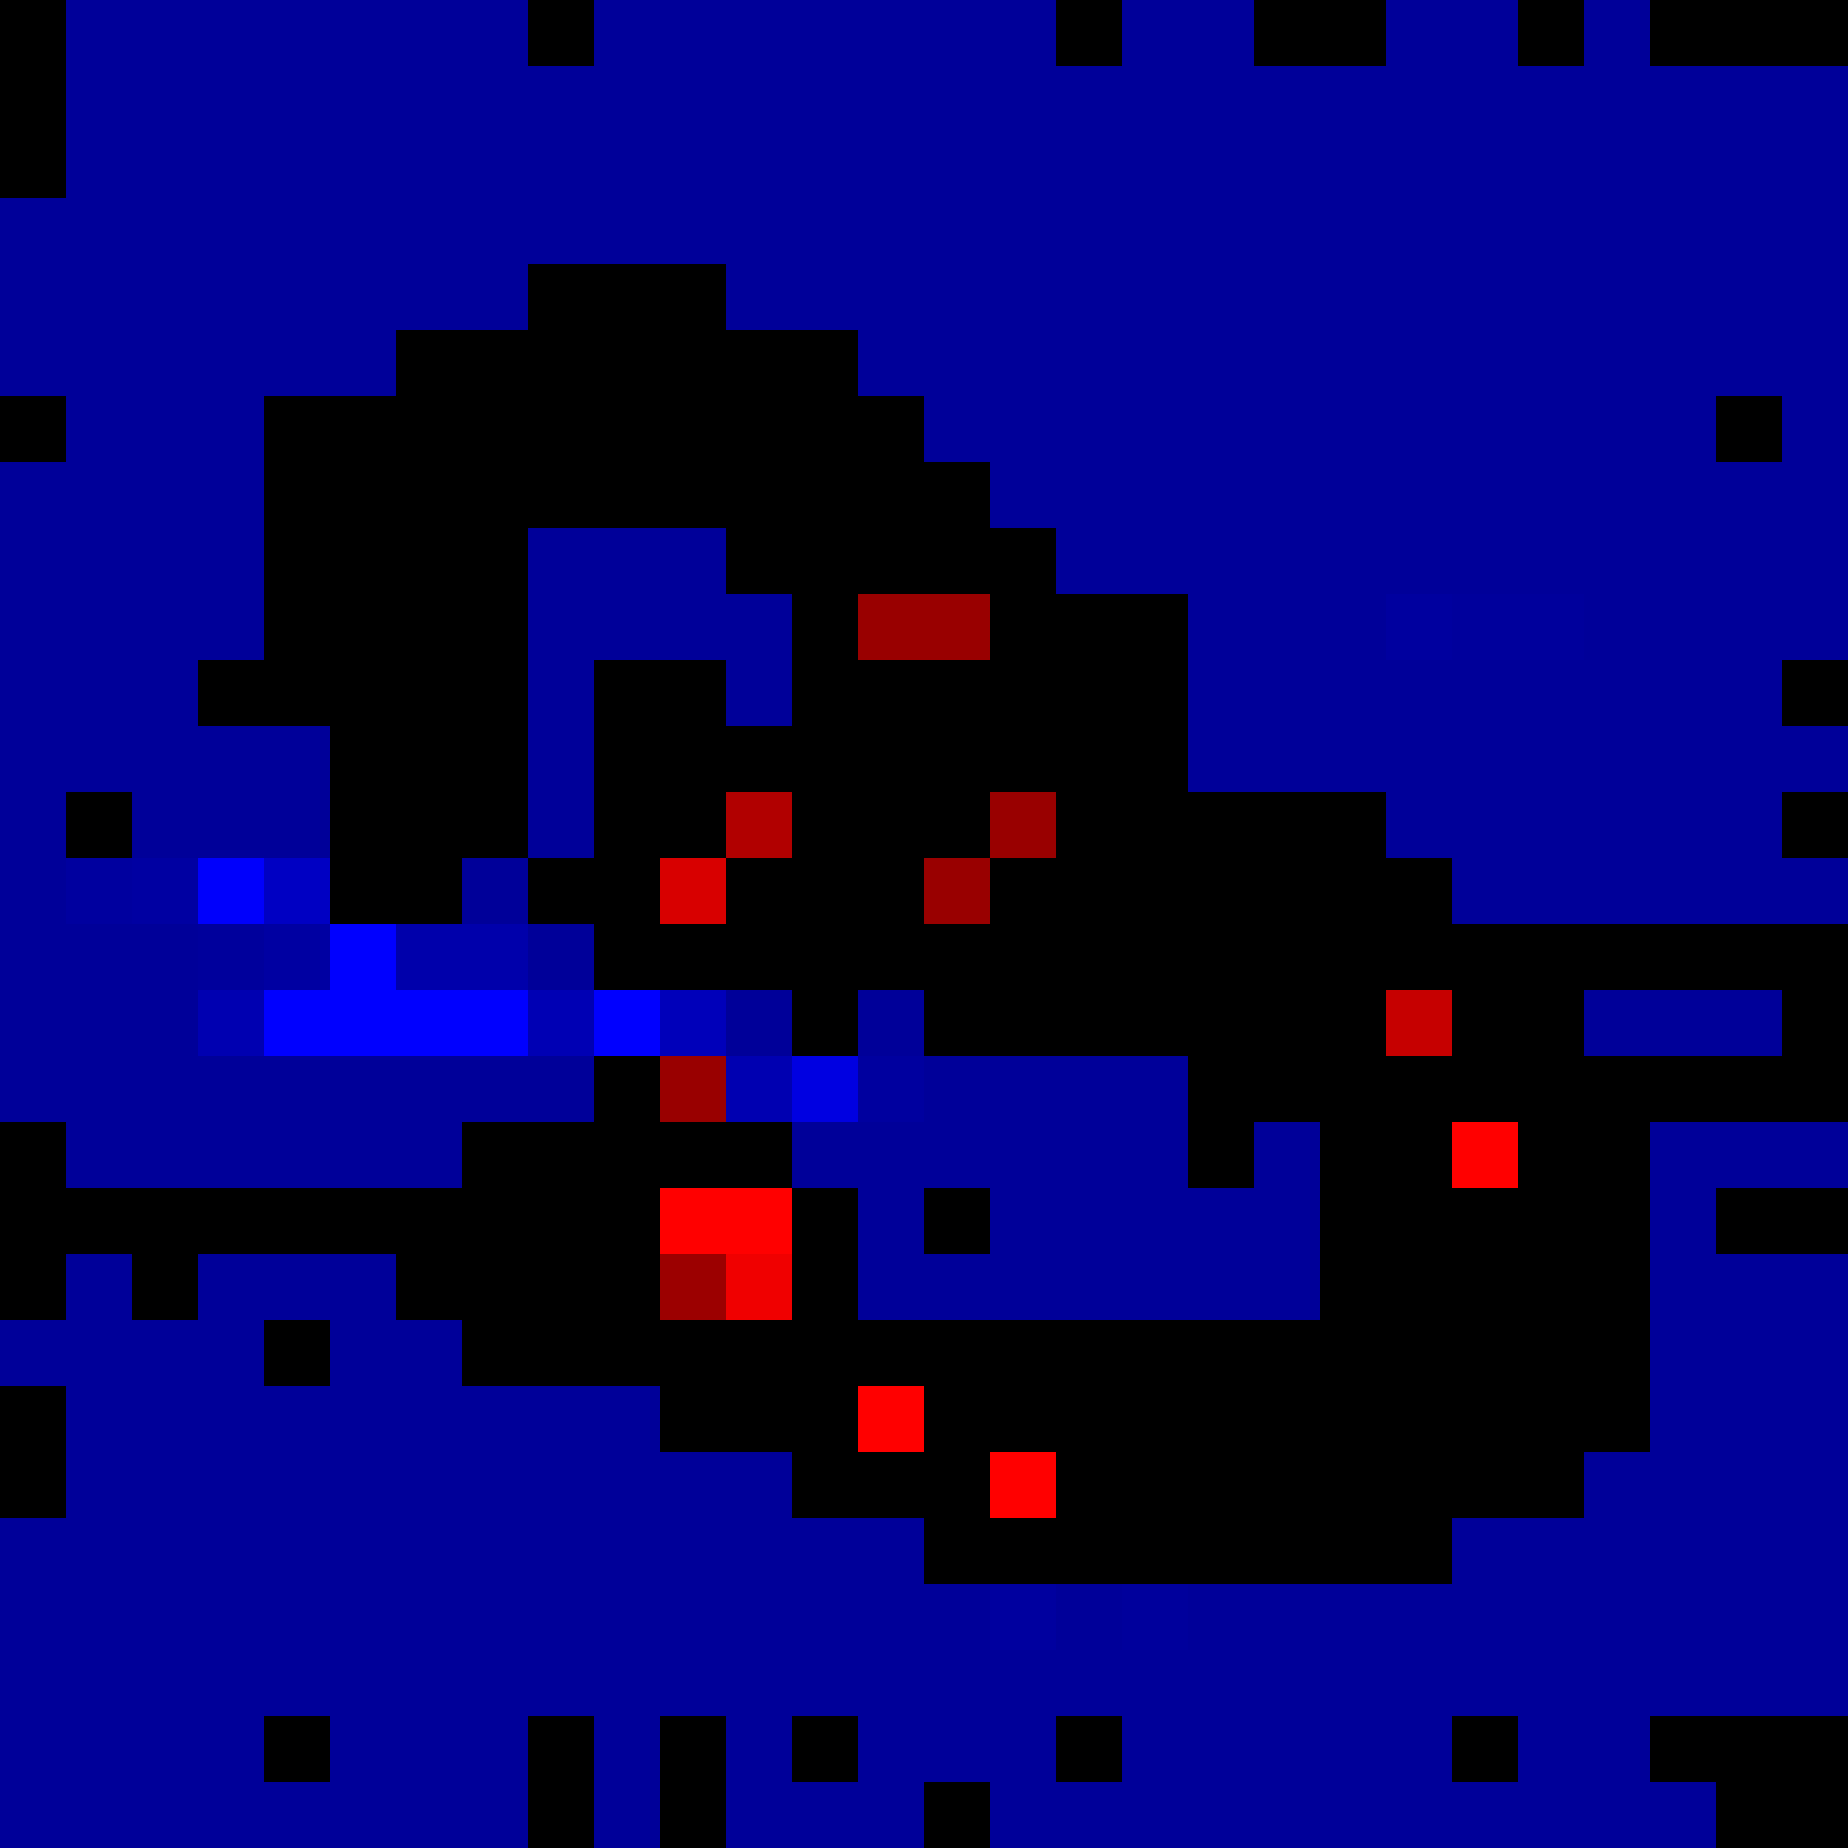
\includegraphics[width=\linewidth]{saliency/mnist_split_ic_saliency/image_030_true_3_pred_3/final_saliency_threshold_wrt_0_bright.png}\\[-1pt]{\scriptsize Logit 0}
		\end{minipage}%
		\begin{minipage}[b]{0.19\linewidth}\centering
			
\includegraphics[width=\linewidth]{saliency/mnist_split_ic_saliency/image_030_true_3_pred_3/final_saliency_threshold_wrt_1_bright.png}\\[-1pt]{\scriptsize Logit 1}
		\end{minipage}%
		\begin{minipage}[b]{0.19\linewidth}\centering
			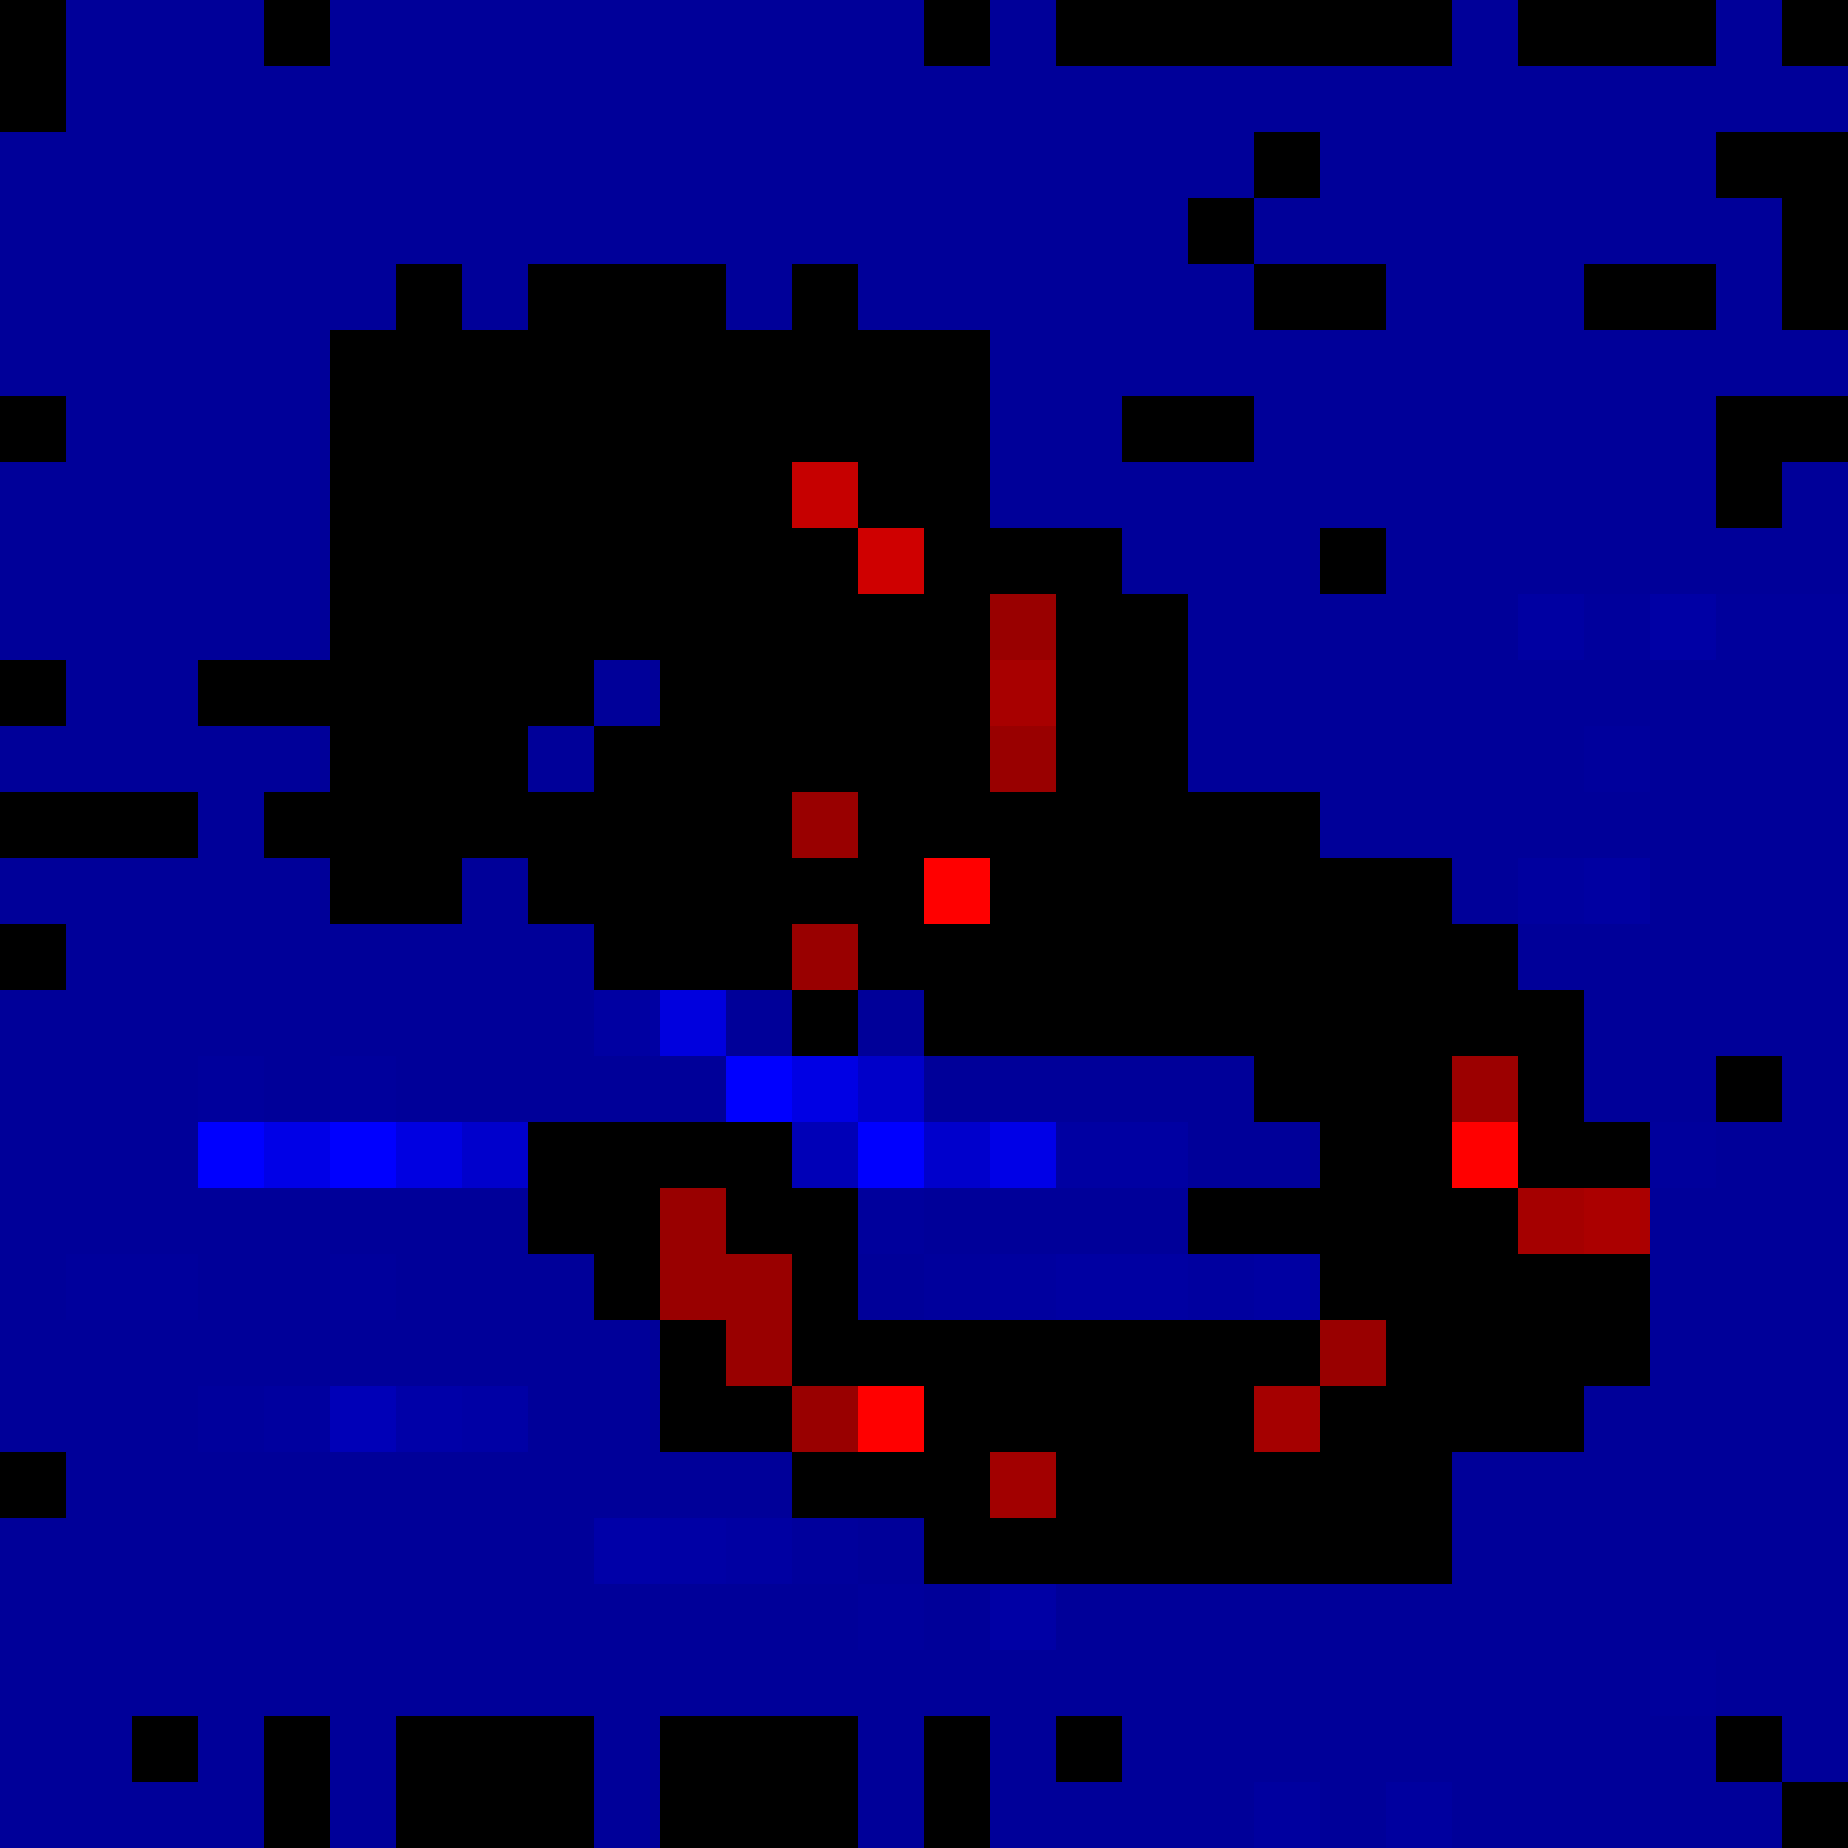
\includegraphics[width=\linewidth]{saliency/mnist_split_ic_saliency/image_030_true_3_pred_3/final_saliency_threshold_wrt_2_bright.png}\\[-1pt]{\scriptsize Logit 2}
		\end{minipage}%
		\begin{minipage}[b]{0.19\linewidth}\centering
			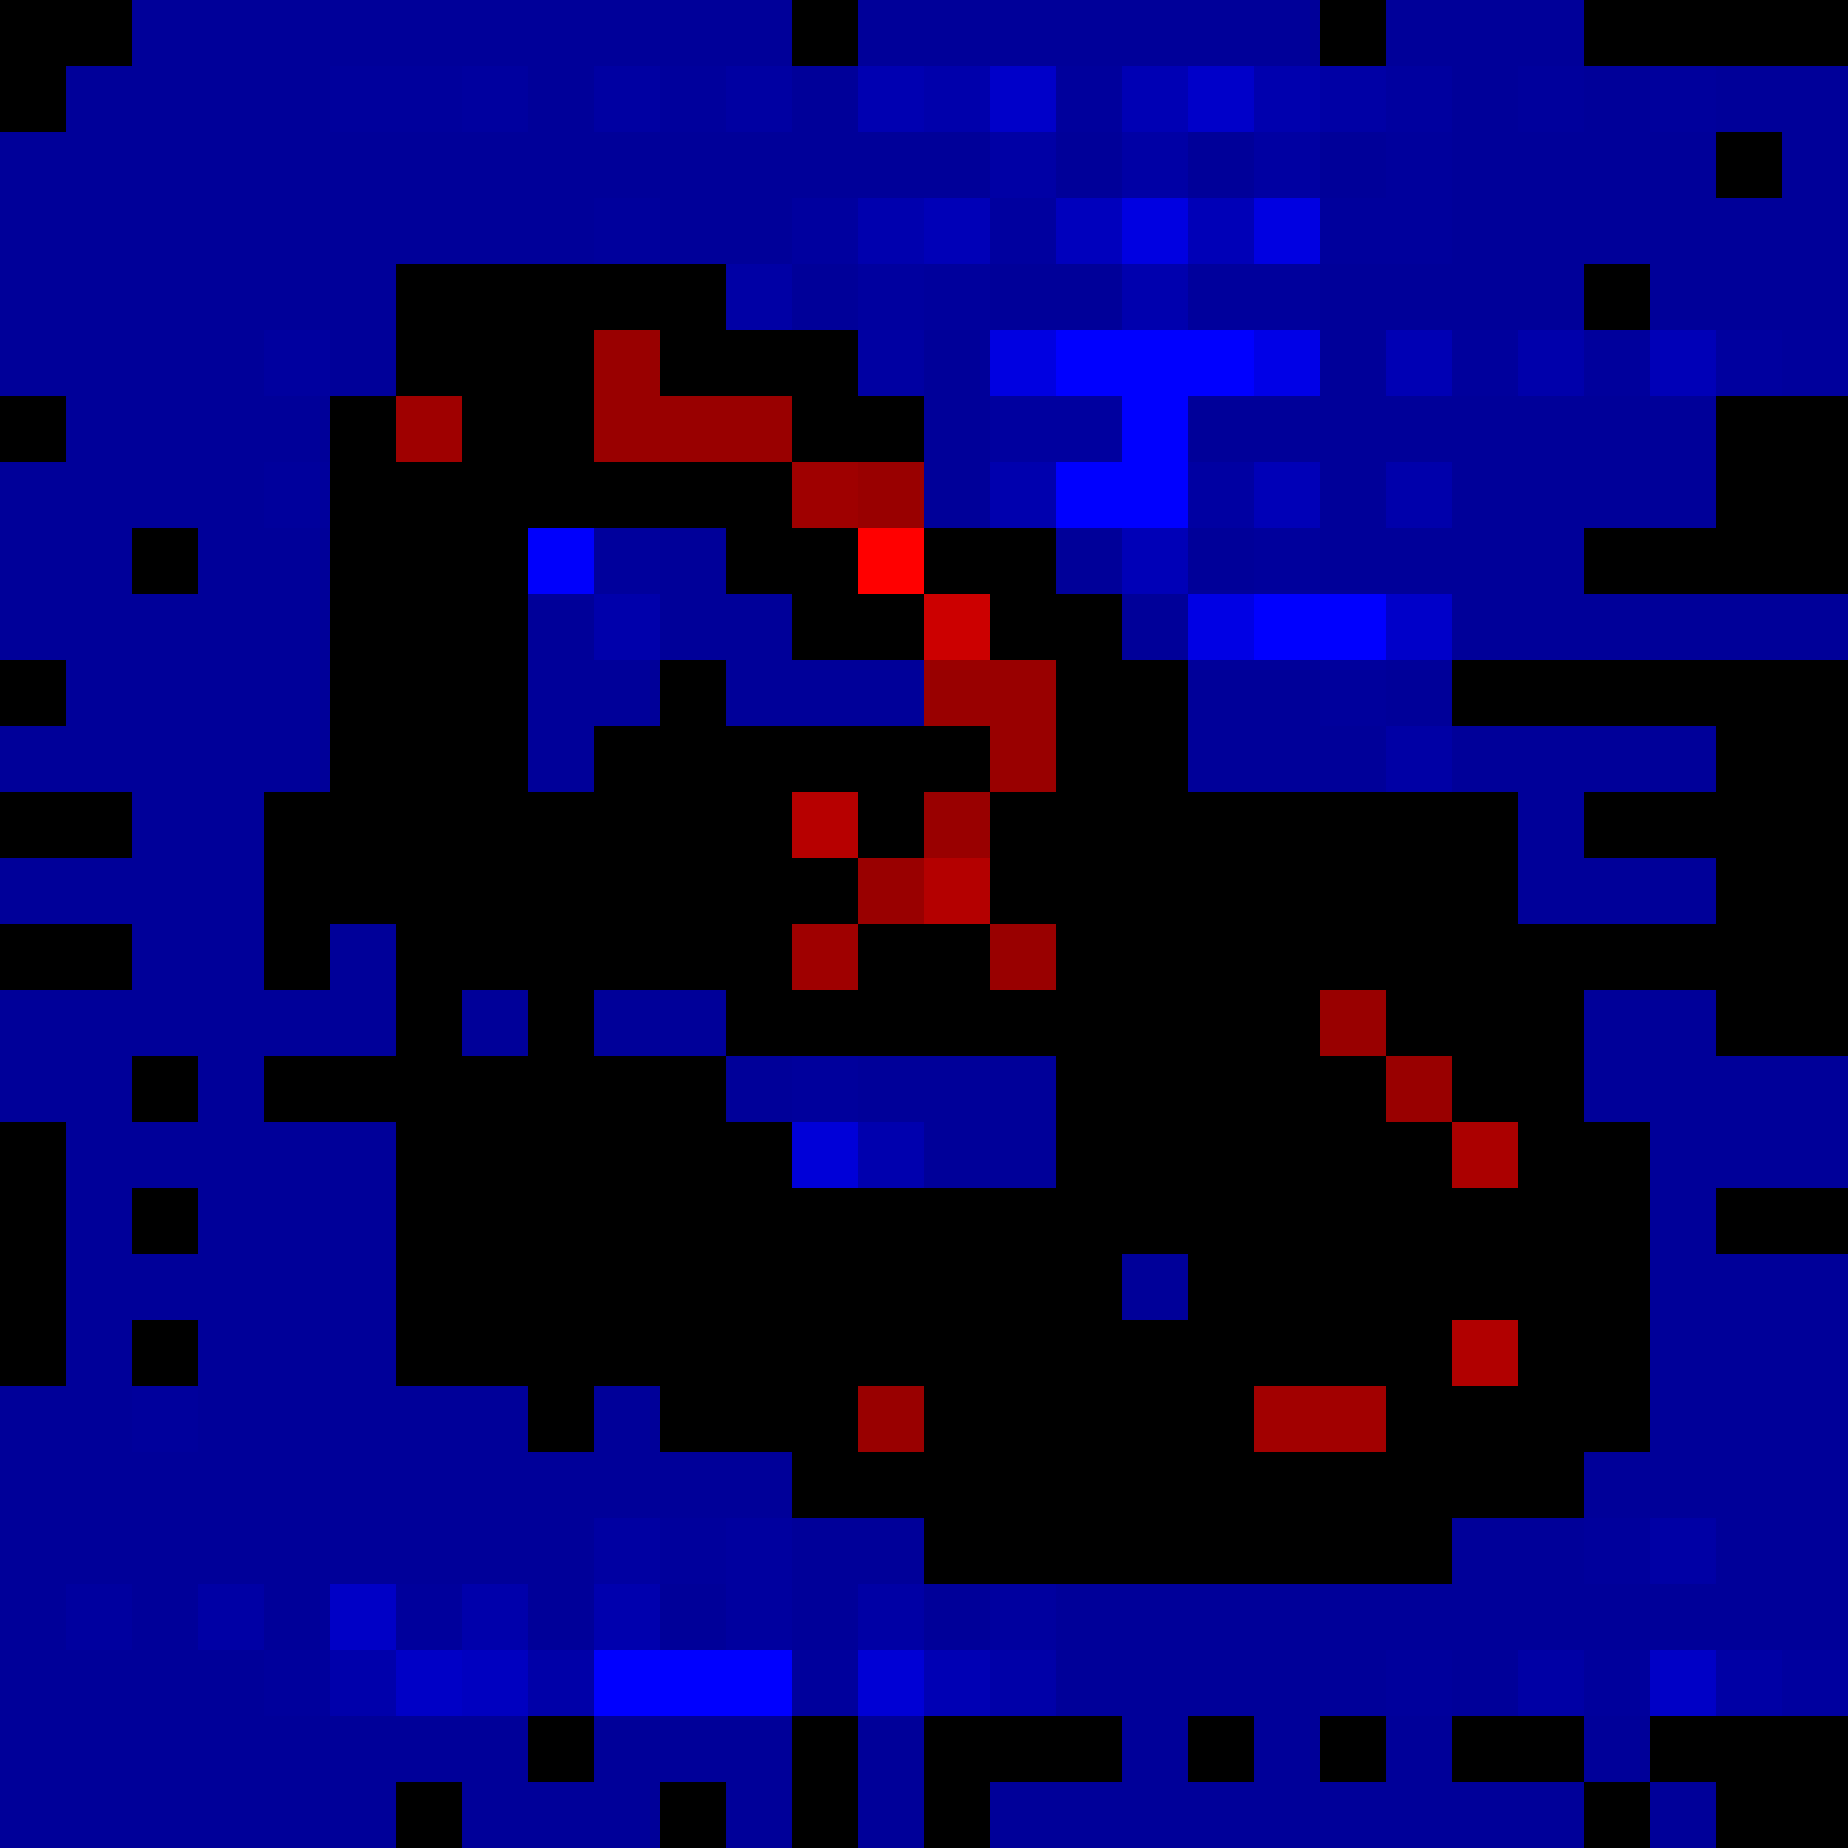
\includegraphics[width=\linewidth]{saliency/mnist_split_ic_saliency/image_030_true_3_pred_3/final_saliency_threshold_wrt_3_bright.png}\\[-1pt]{\scriptsize Logit 3}
		\end{minipage}%
		\begin{minipage}[b]{0.19\linewidth}\centering
			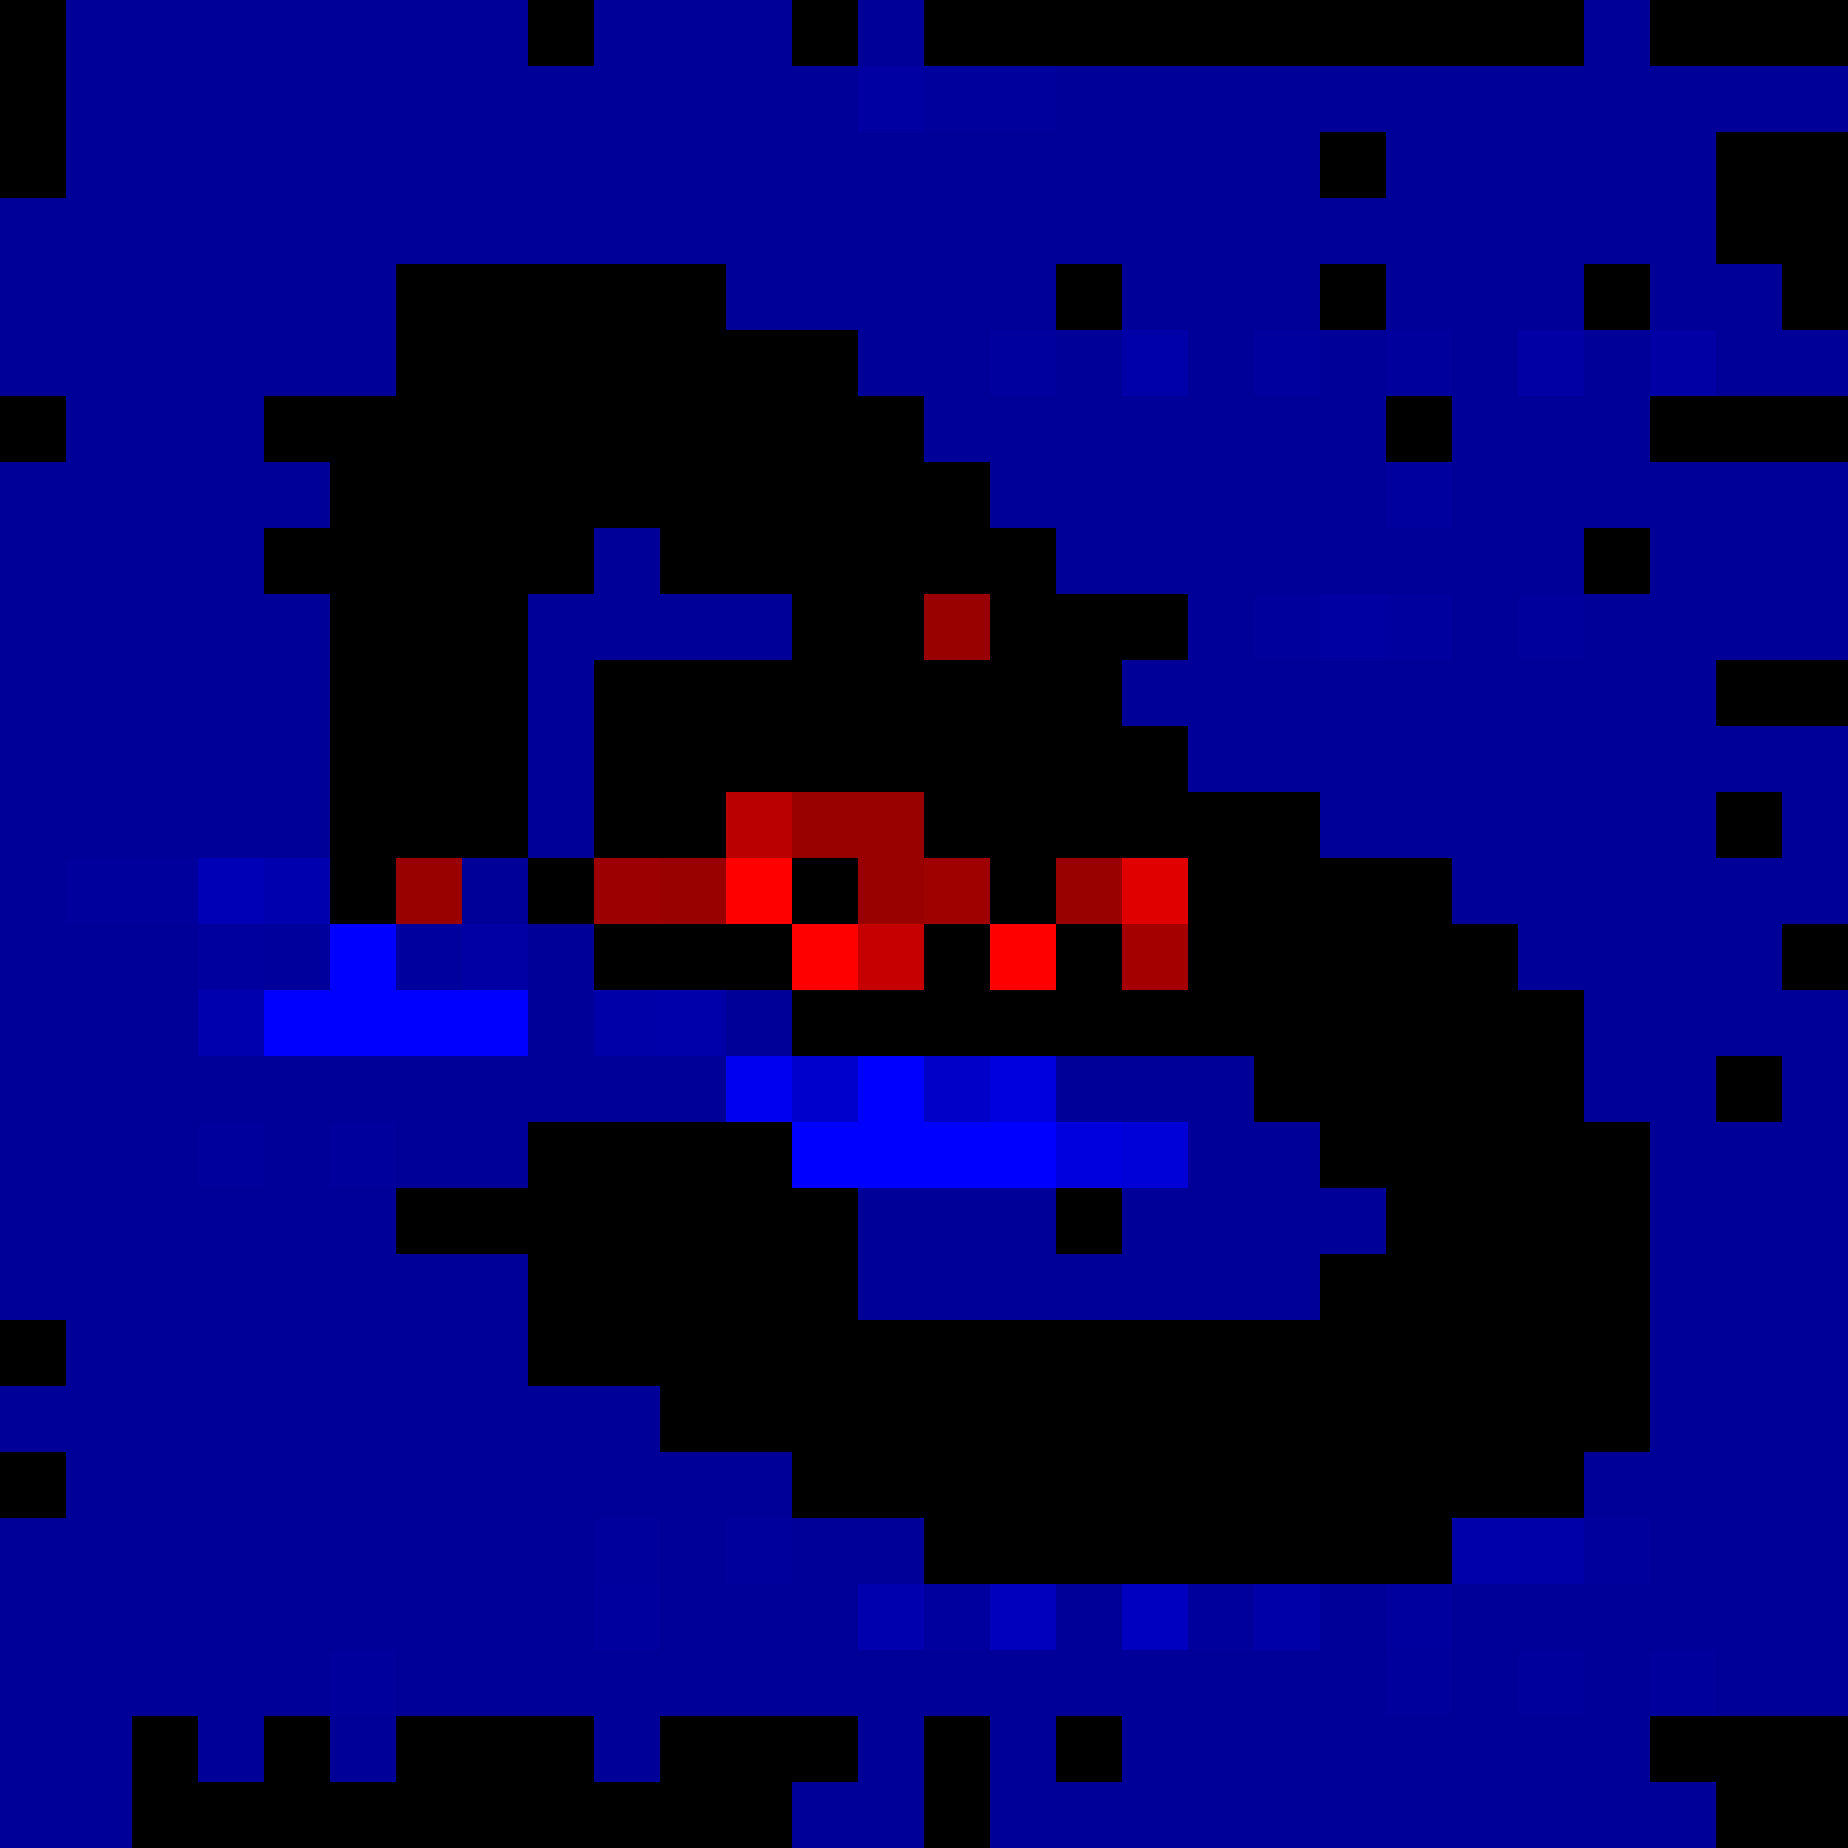
\includegraphics[width=\linewidth]{saliency/mnist_split_ic_saliency/image_030_true_3_pred_3/final_saliency_threshold_wrt_4_bright.png}\\[-1pt]{\scriptsize Logit 4}
		\end{minipage}

		\vspace{0.12cm}

		\begin{minipage}[b]{0.19\linewidth}\centering
			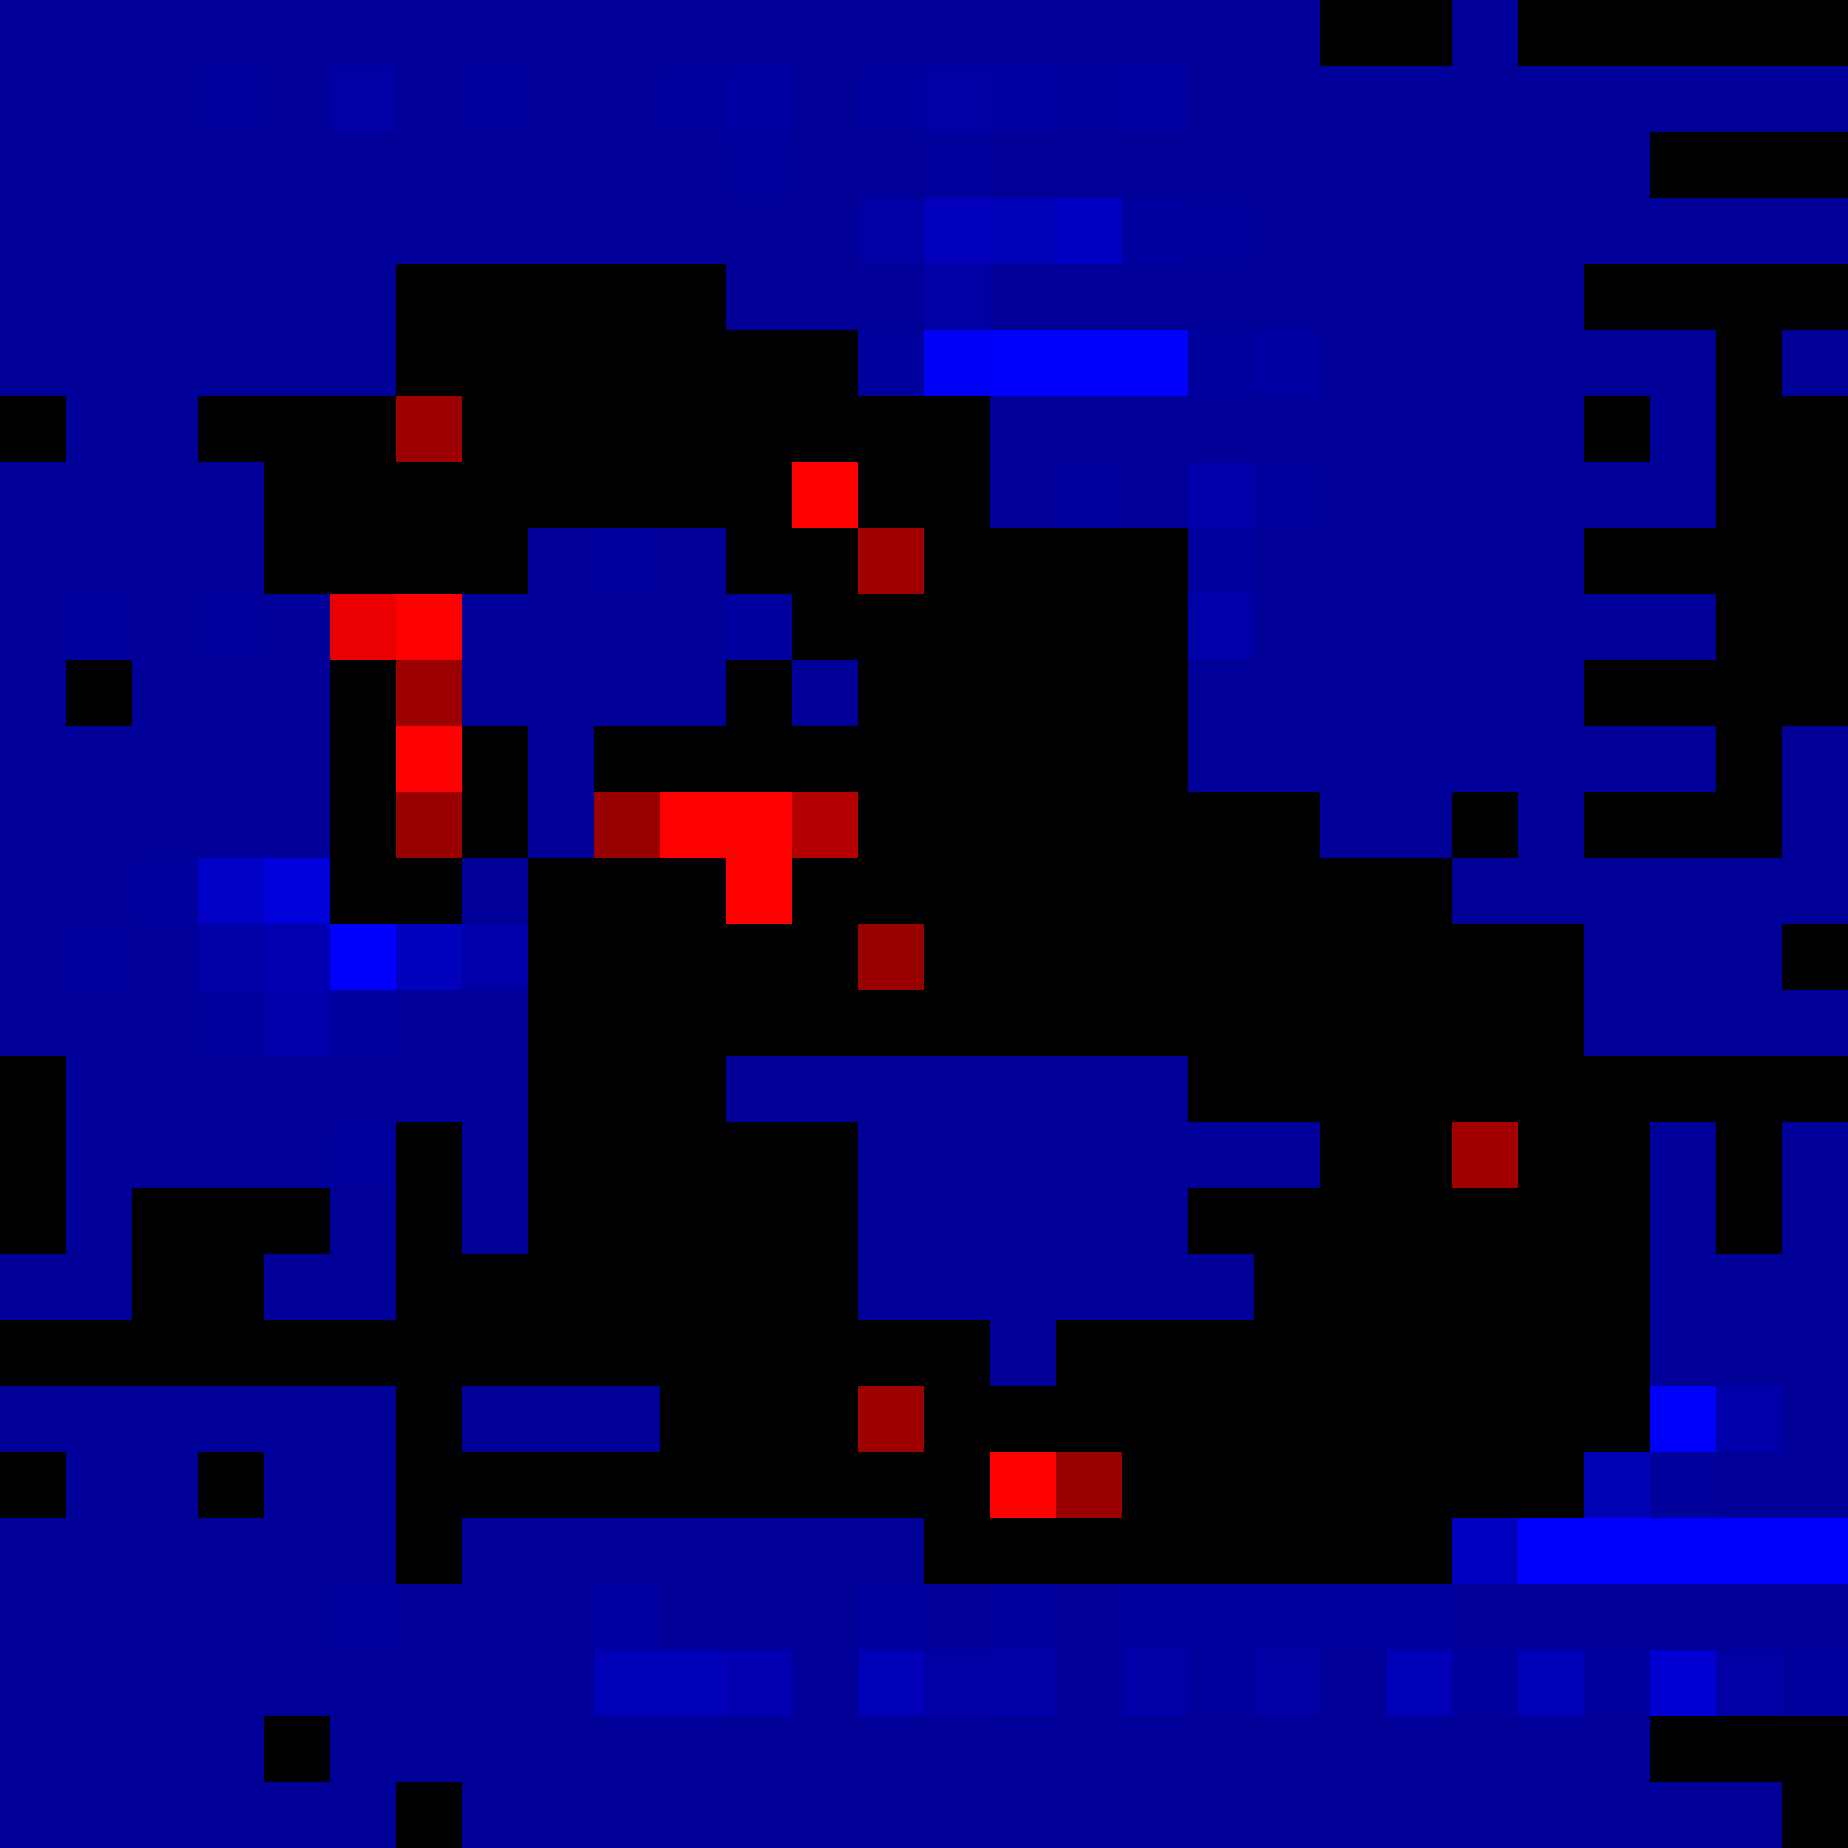
\includegraphics[width=\linewidth]{saliency/mnist_split_ic_saliency/image_030_true_3_pred_3/final_saliency_threshold_wrt_5_bright.png}\\[-1pt]{\scriptsize Logit 5}
		\end{minipage}%
		\begin{minipage}[b]{0.19\linewidth}\centering
			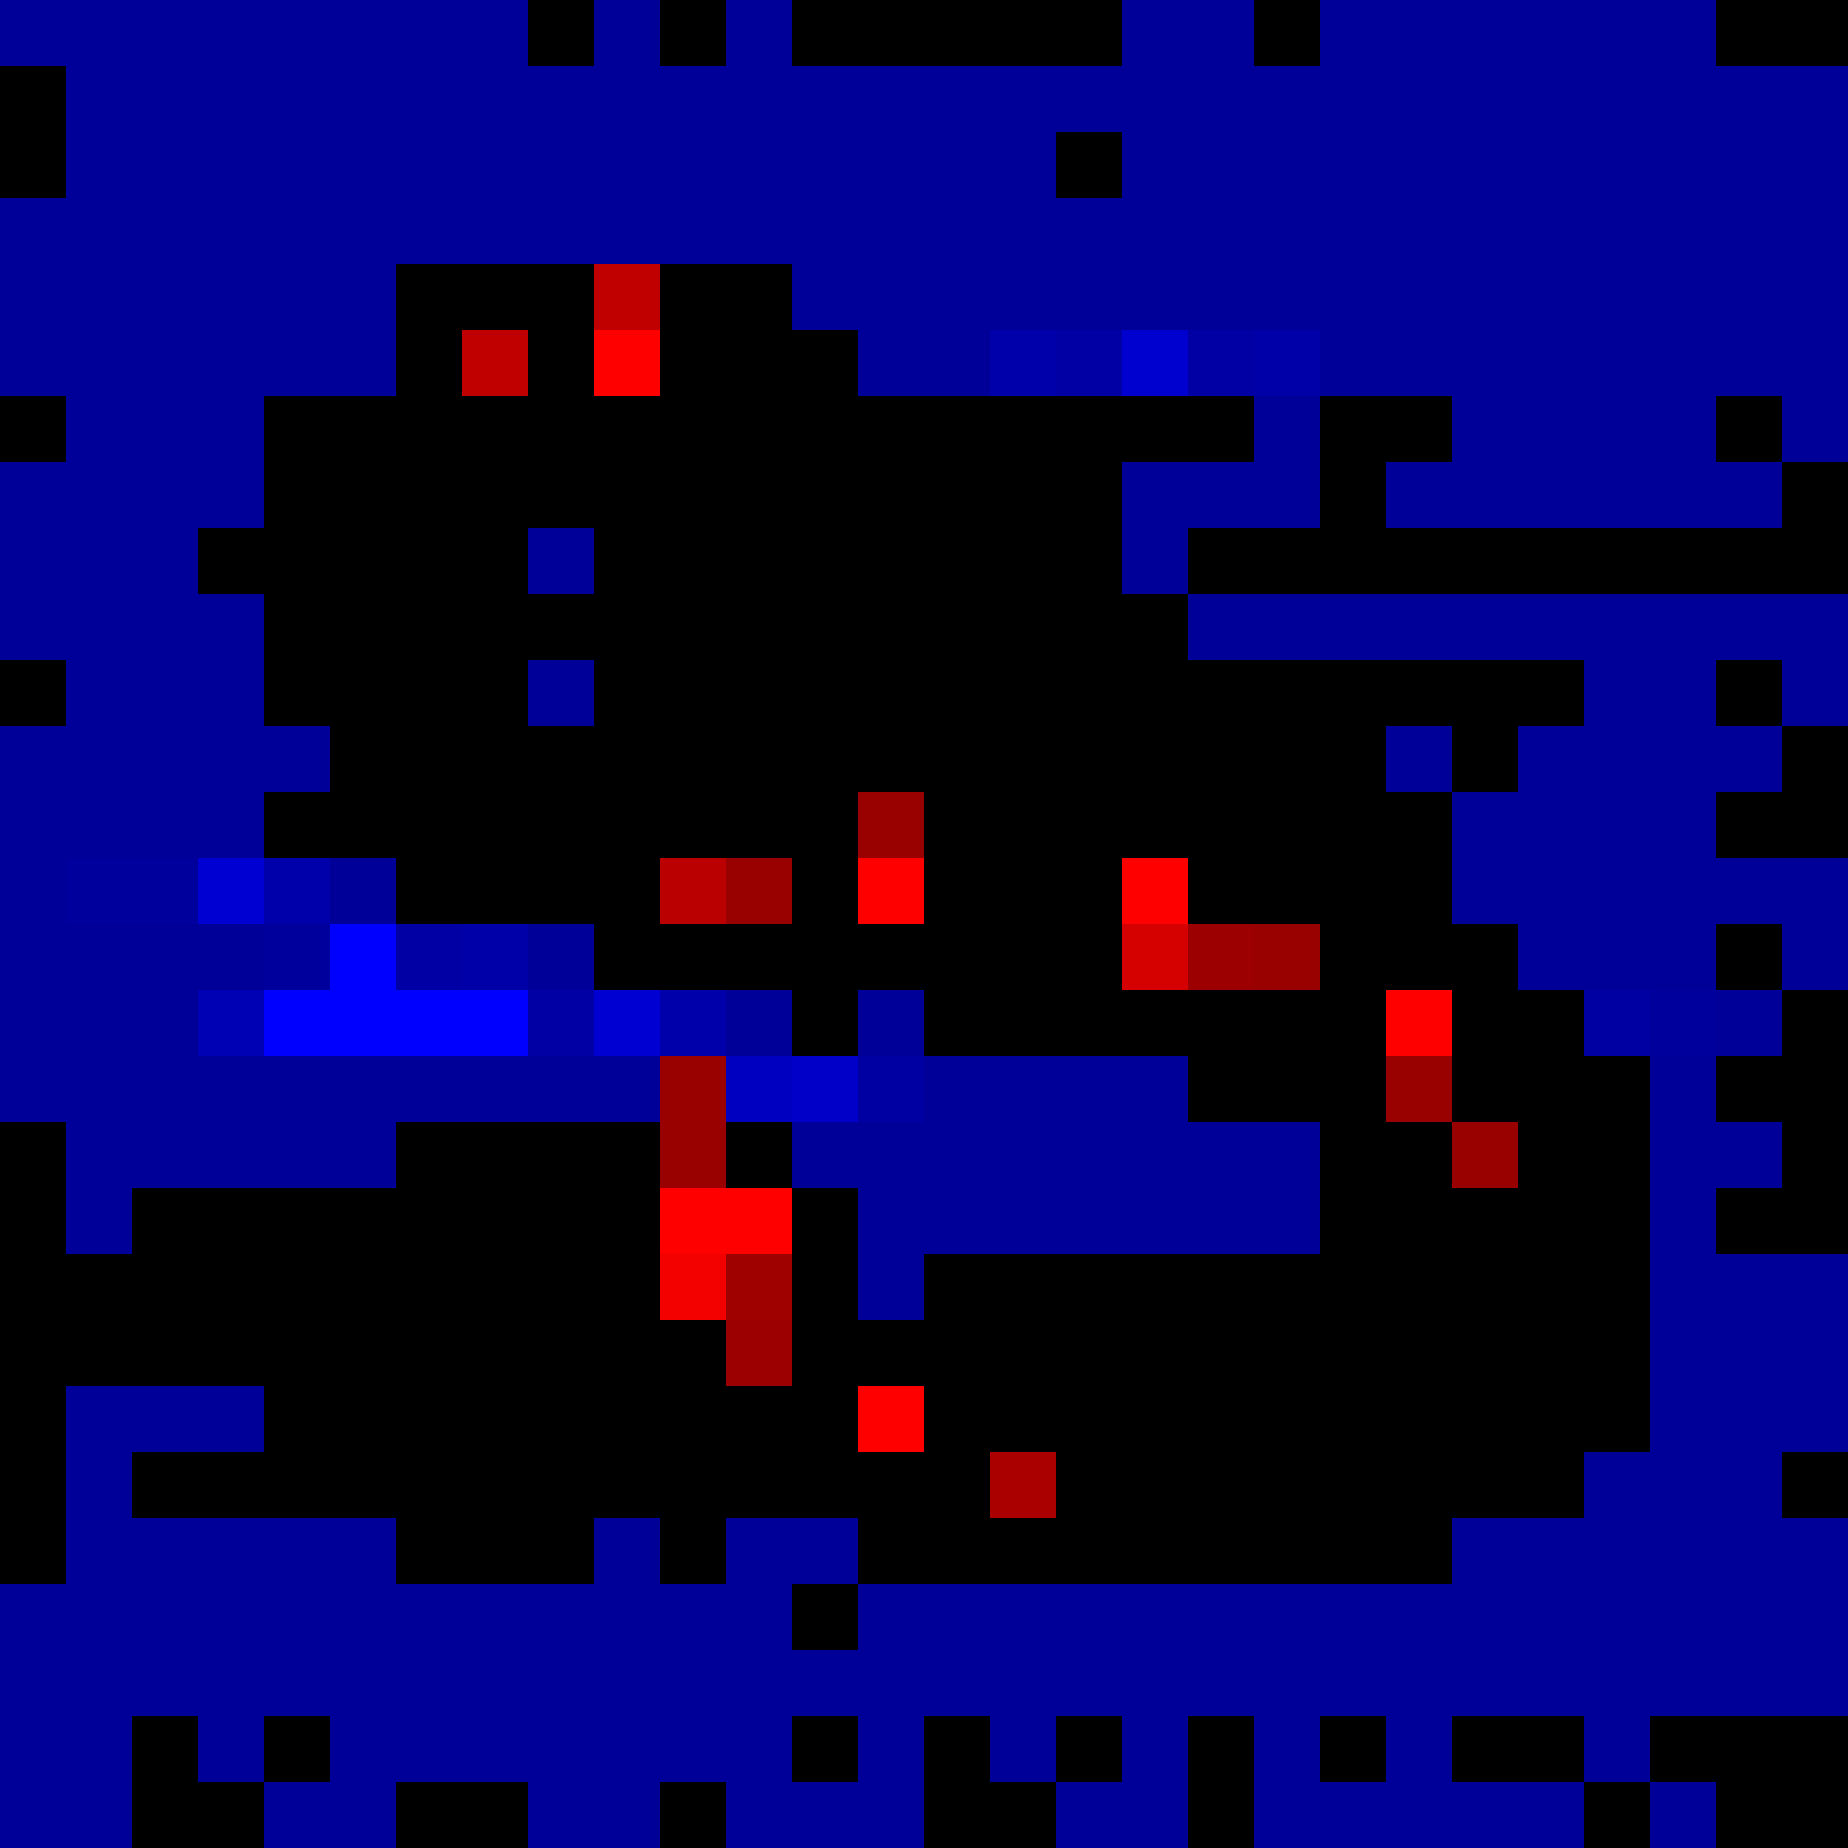
\includegraphics[width=\linewidth]{saliency/mnist_split_ic_saliency/image_030_true_3_pred_3/final_saliency_threshold_wrt_6_bright.png}\\[-1pt]{\scriptsize Logit 6}
		\end{minipage}%
		\begin{minipage}[b]{0.19\linewidth}\centering
			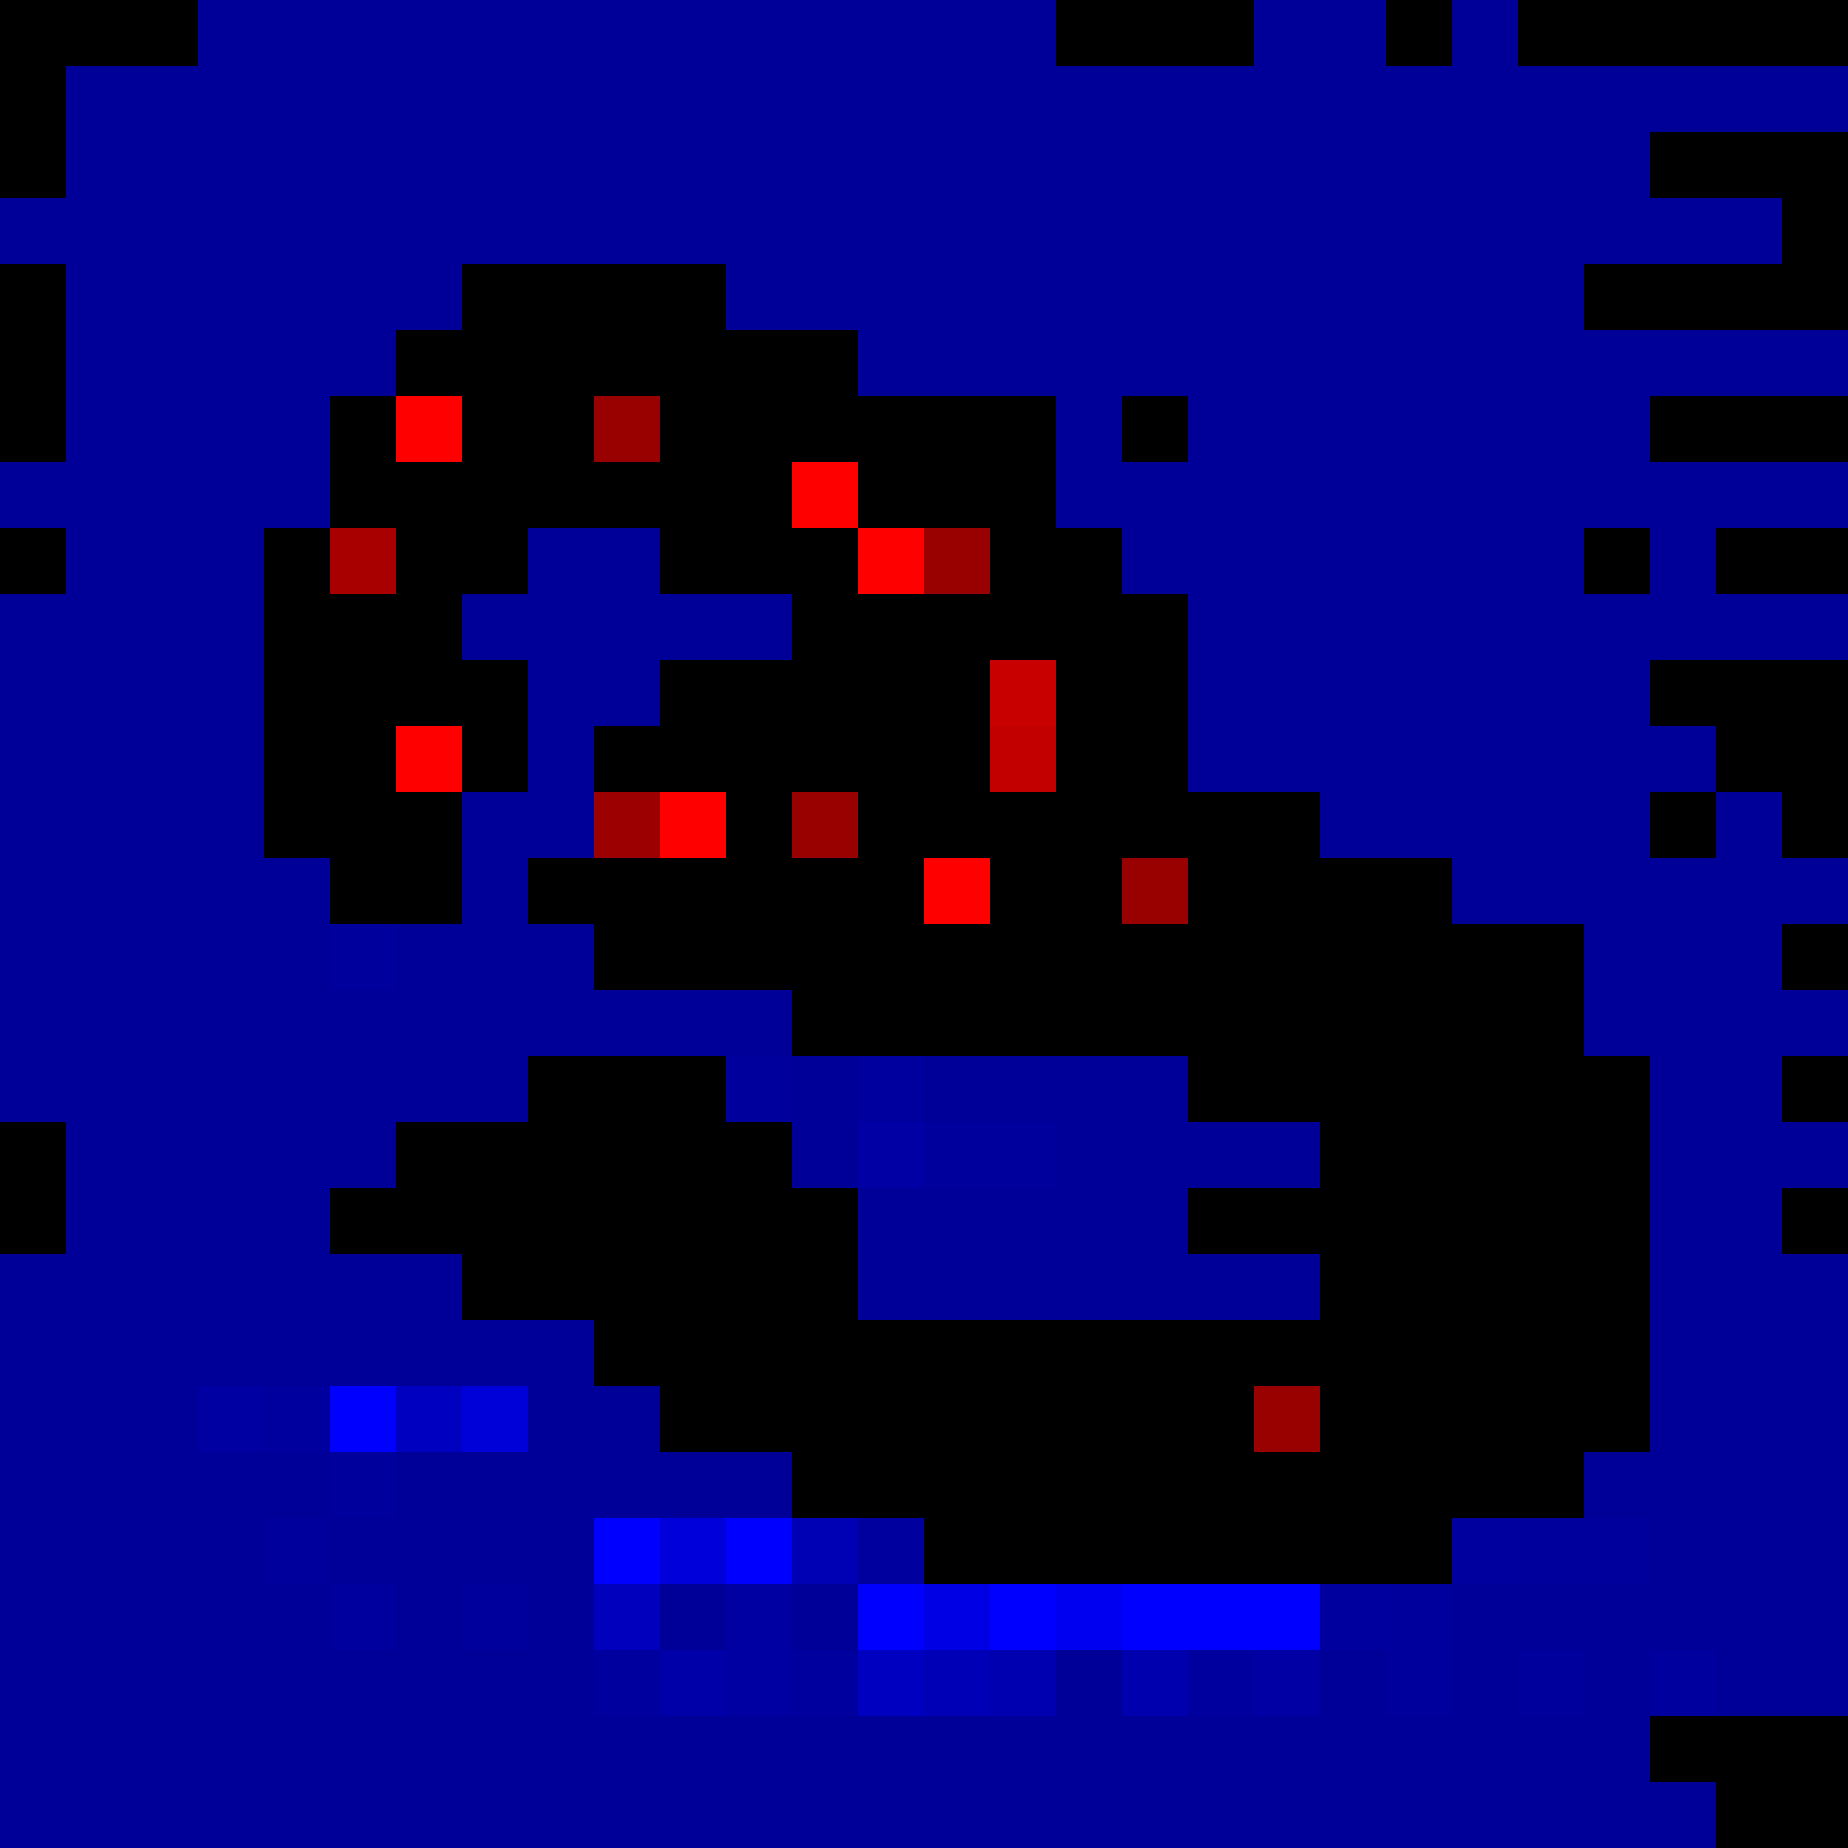
\includegraphics[width=\linewidth]{saliency/mnist_split_ic_saliency/image_030_true_3_pred_3/final_saliency_threshold_wrt_7_bright.png}\\[-1pt]{\scriptsize Logit 7}
		\end{minipage}%
		\begin{minipage}[b]{0.19\linewidth}\centering
			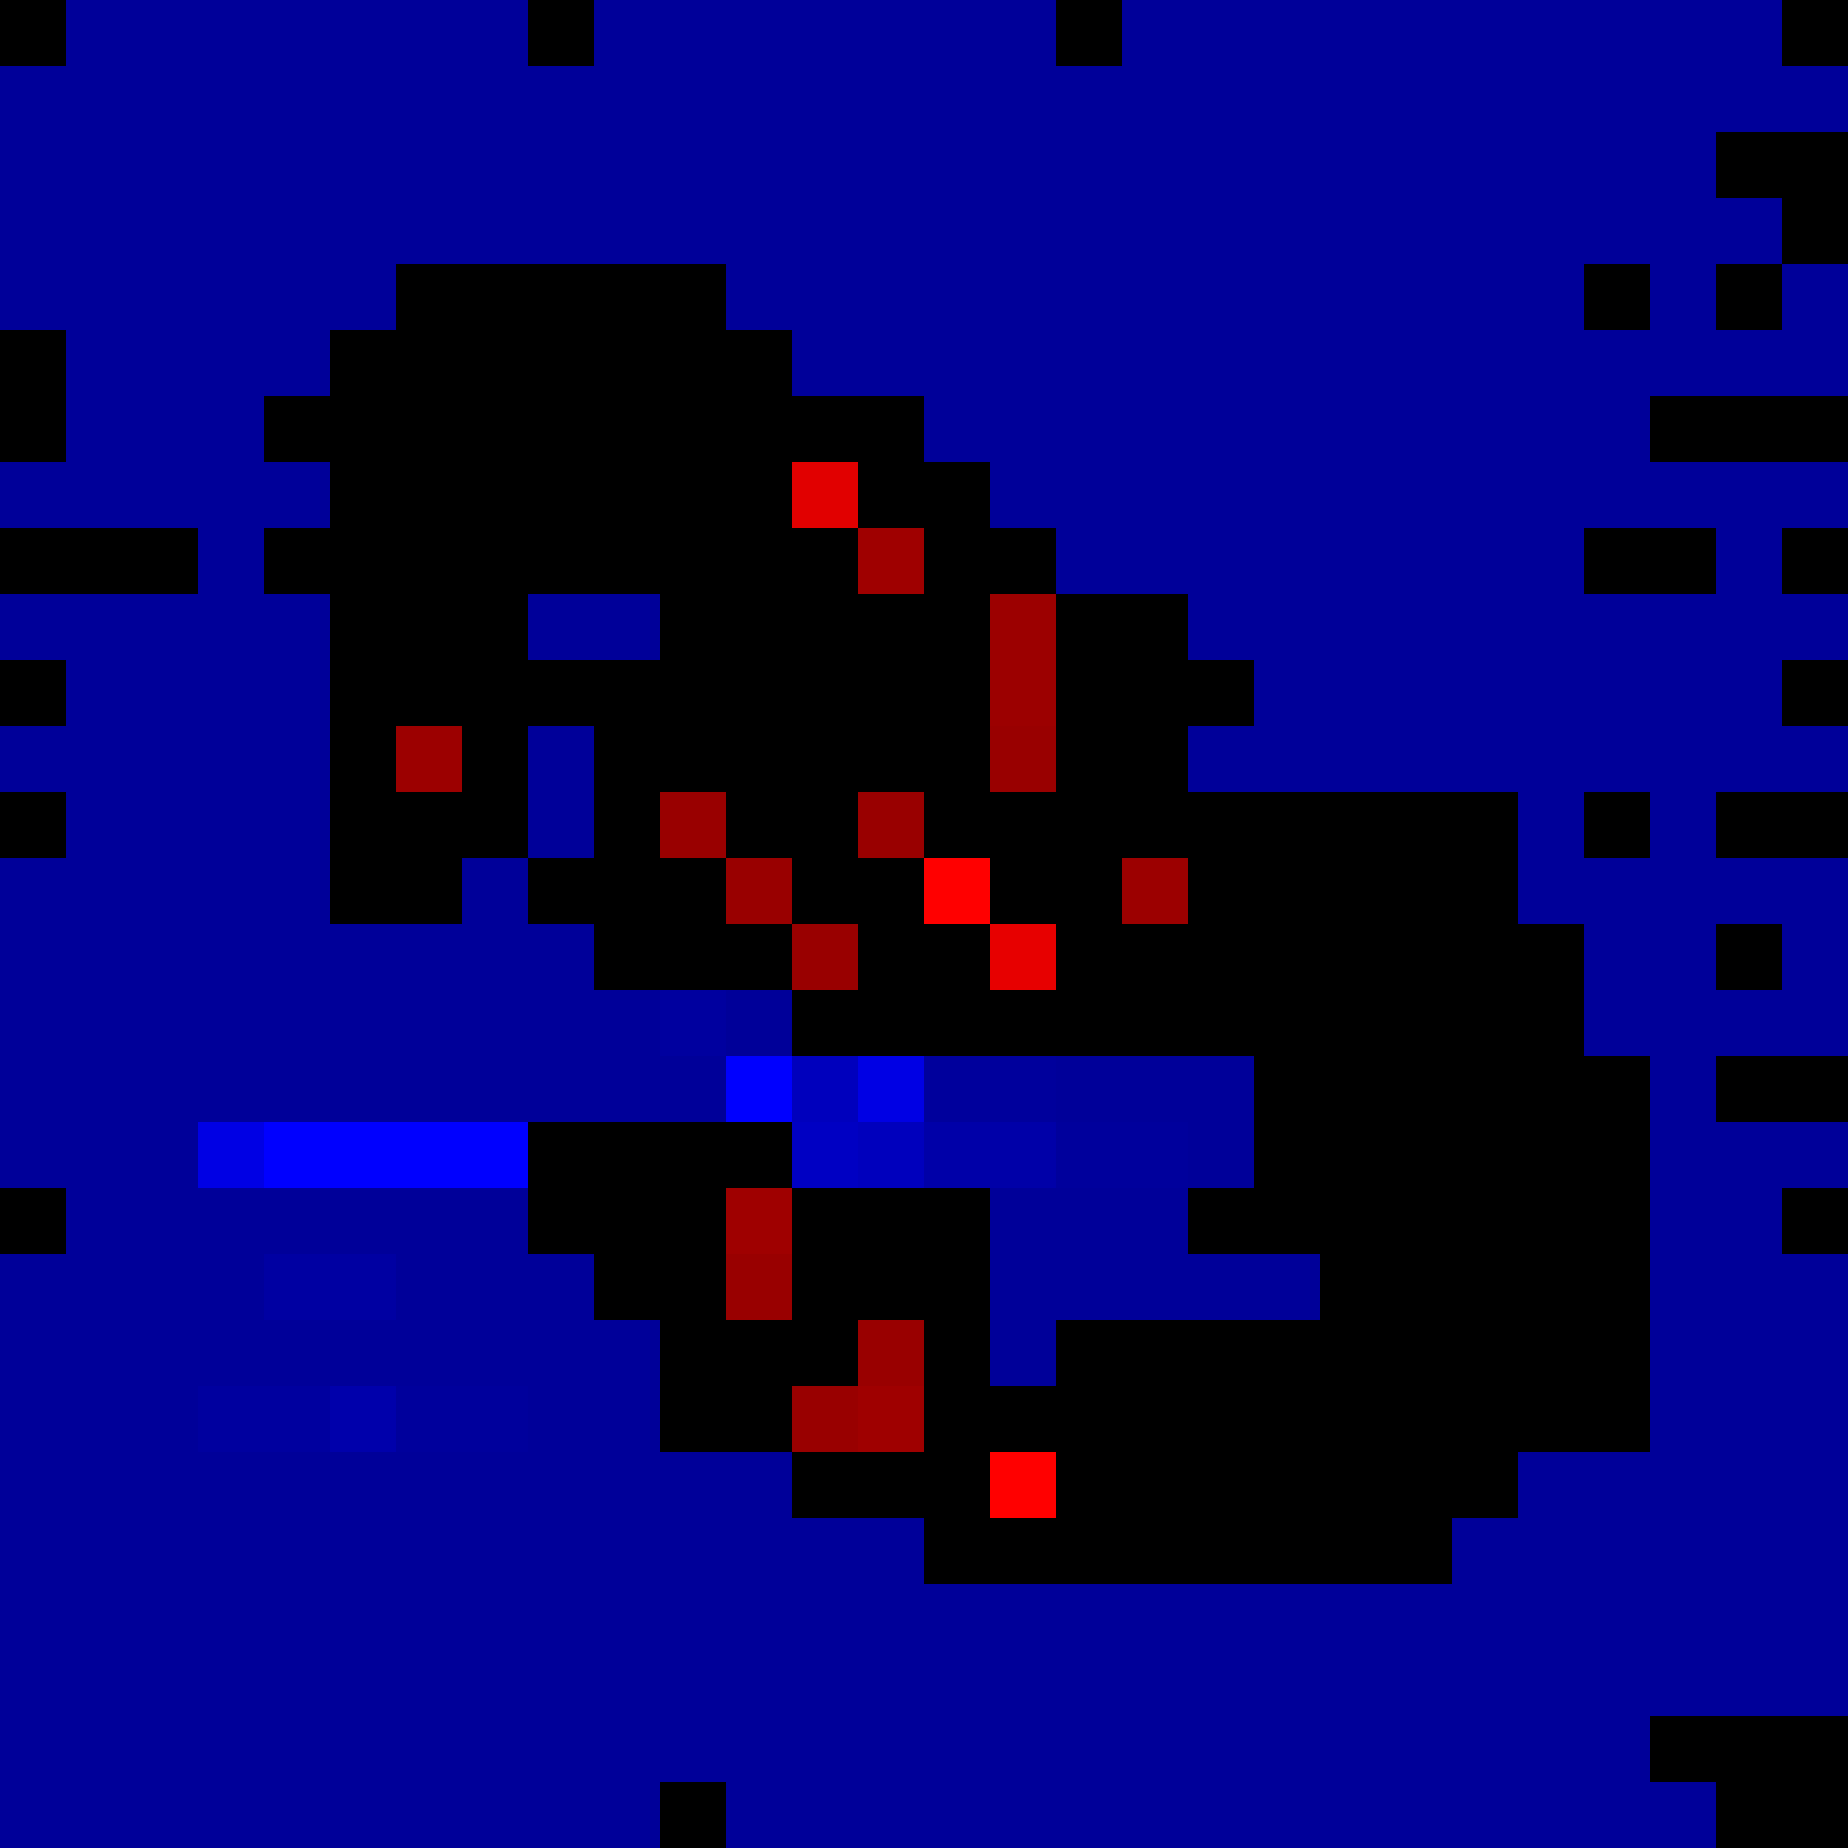
\includegraphics[width=\linewidth]{saliency/mnist_split_ic_saliency/image_030_true_3_pred_3/final_saliency_threshold_wrt_8_bright.png}\\[-1pt]{\scriptsize Logit 8}
		\end{minipage}%
		\begin{minipage}[b]{0.19\linewidth}\centering
			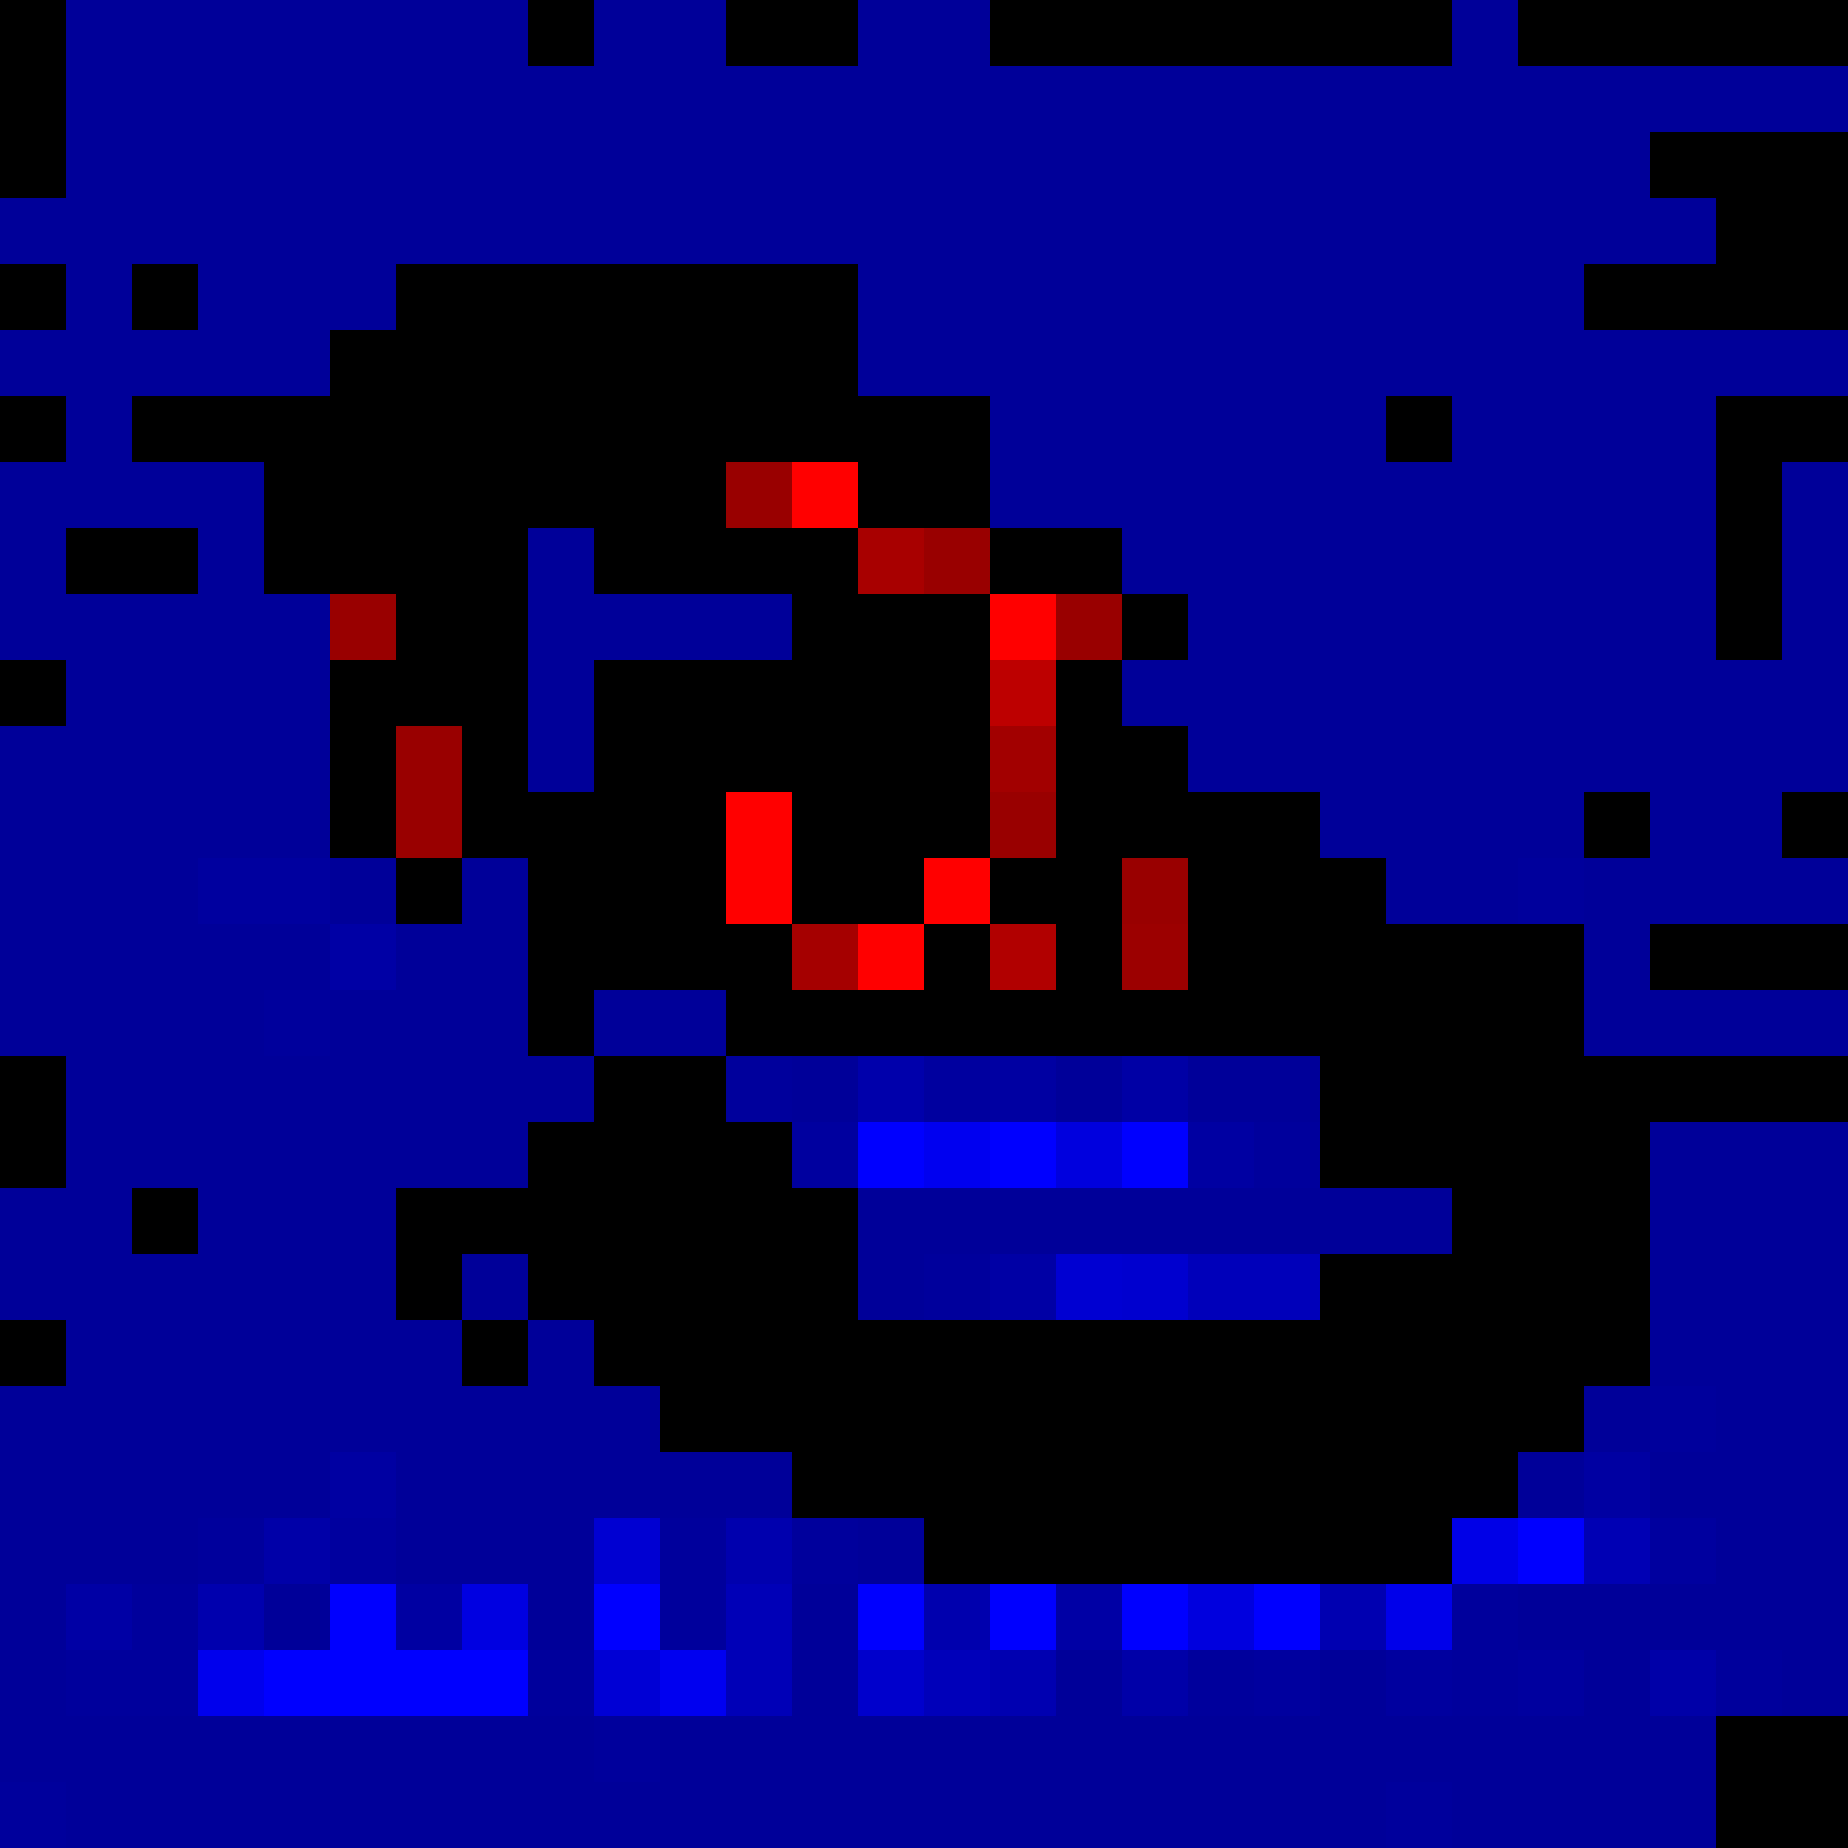
\includegraphics[width=\linewidth]{saliency/mnist_split_ic_saliency/image_030_true_3_pred_3/final_saliency_threshold_wrt_9_bright.png}\\[-1pt]{\scriptsize Logit 9}
		\end{minipage}
	\end{minipage}
	}%
\caption[Stream gradients of the inverted-input DIC model]{Stream gradients of the inverted-input DIC model (\texttt{cnn\_maxout} DICIN) on a correctly classified MNIST test digit ``3'', thresholded and overlaid per class logit. The $g$-stream gradient (red) highlights sensitivities on present strokes, while the $h$-stream gradient (blue) highlights sensitivities at candidate missing-stroke locations. Left: the original digit.}
	\label{fig:mnist_split_ic_saliency}
\end{figure}

\begin{figure}[t]
\QualitativeImageContent{
	\centering
	\begin{minipage}[c]{0.15\linewidth}
		\centering
		
\includegraphics[width=\linewidth]{saliency/mnist_split_ic_saliency/image_036_true_3_pred_3/original.png}\\[-1pt]
		{\scriptsize Original}
	\end{minipage}\hspace{0.015\linewidth}%
	\begin{minipage}[c]{0.80\linewidth}
		\centering
		\begin{minipage}[b]{0.19\linewidth}\centering
			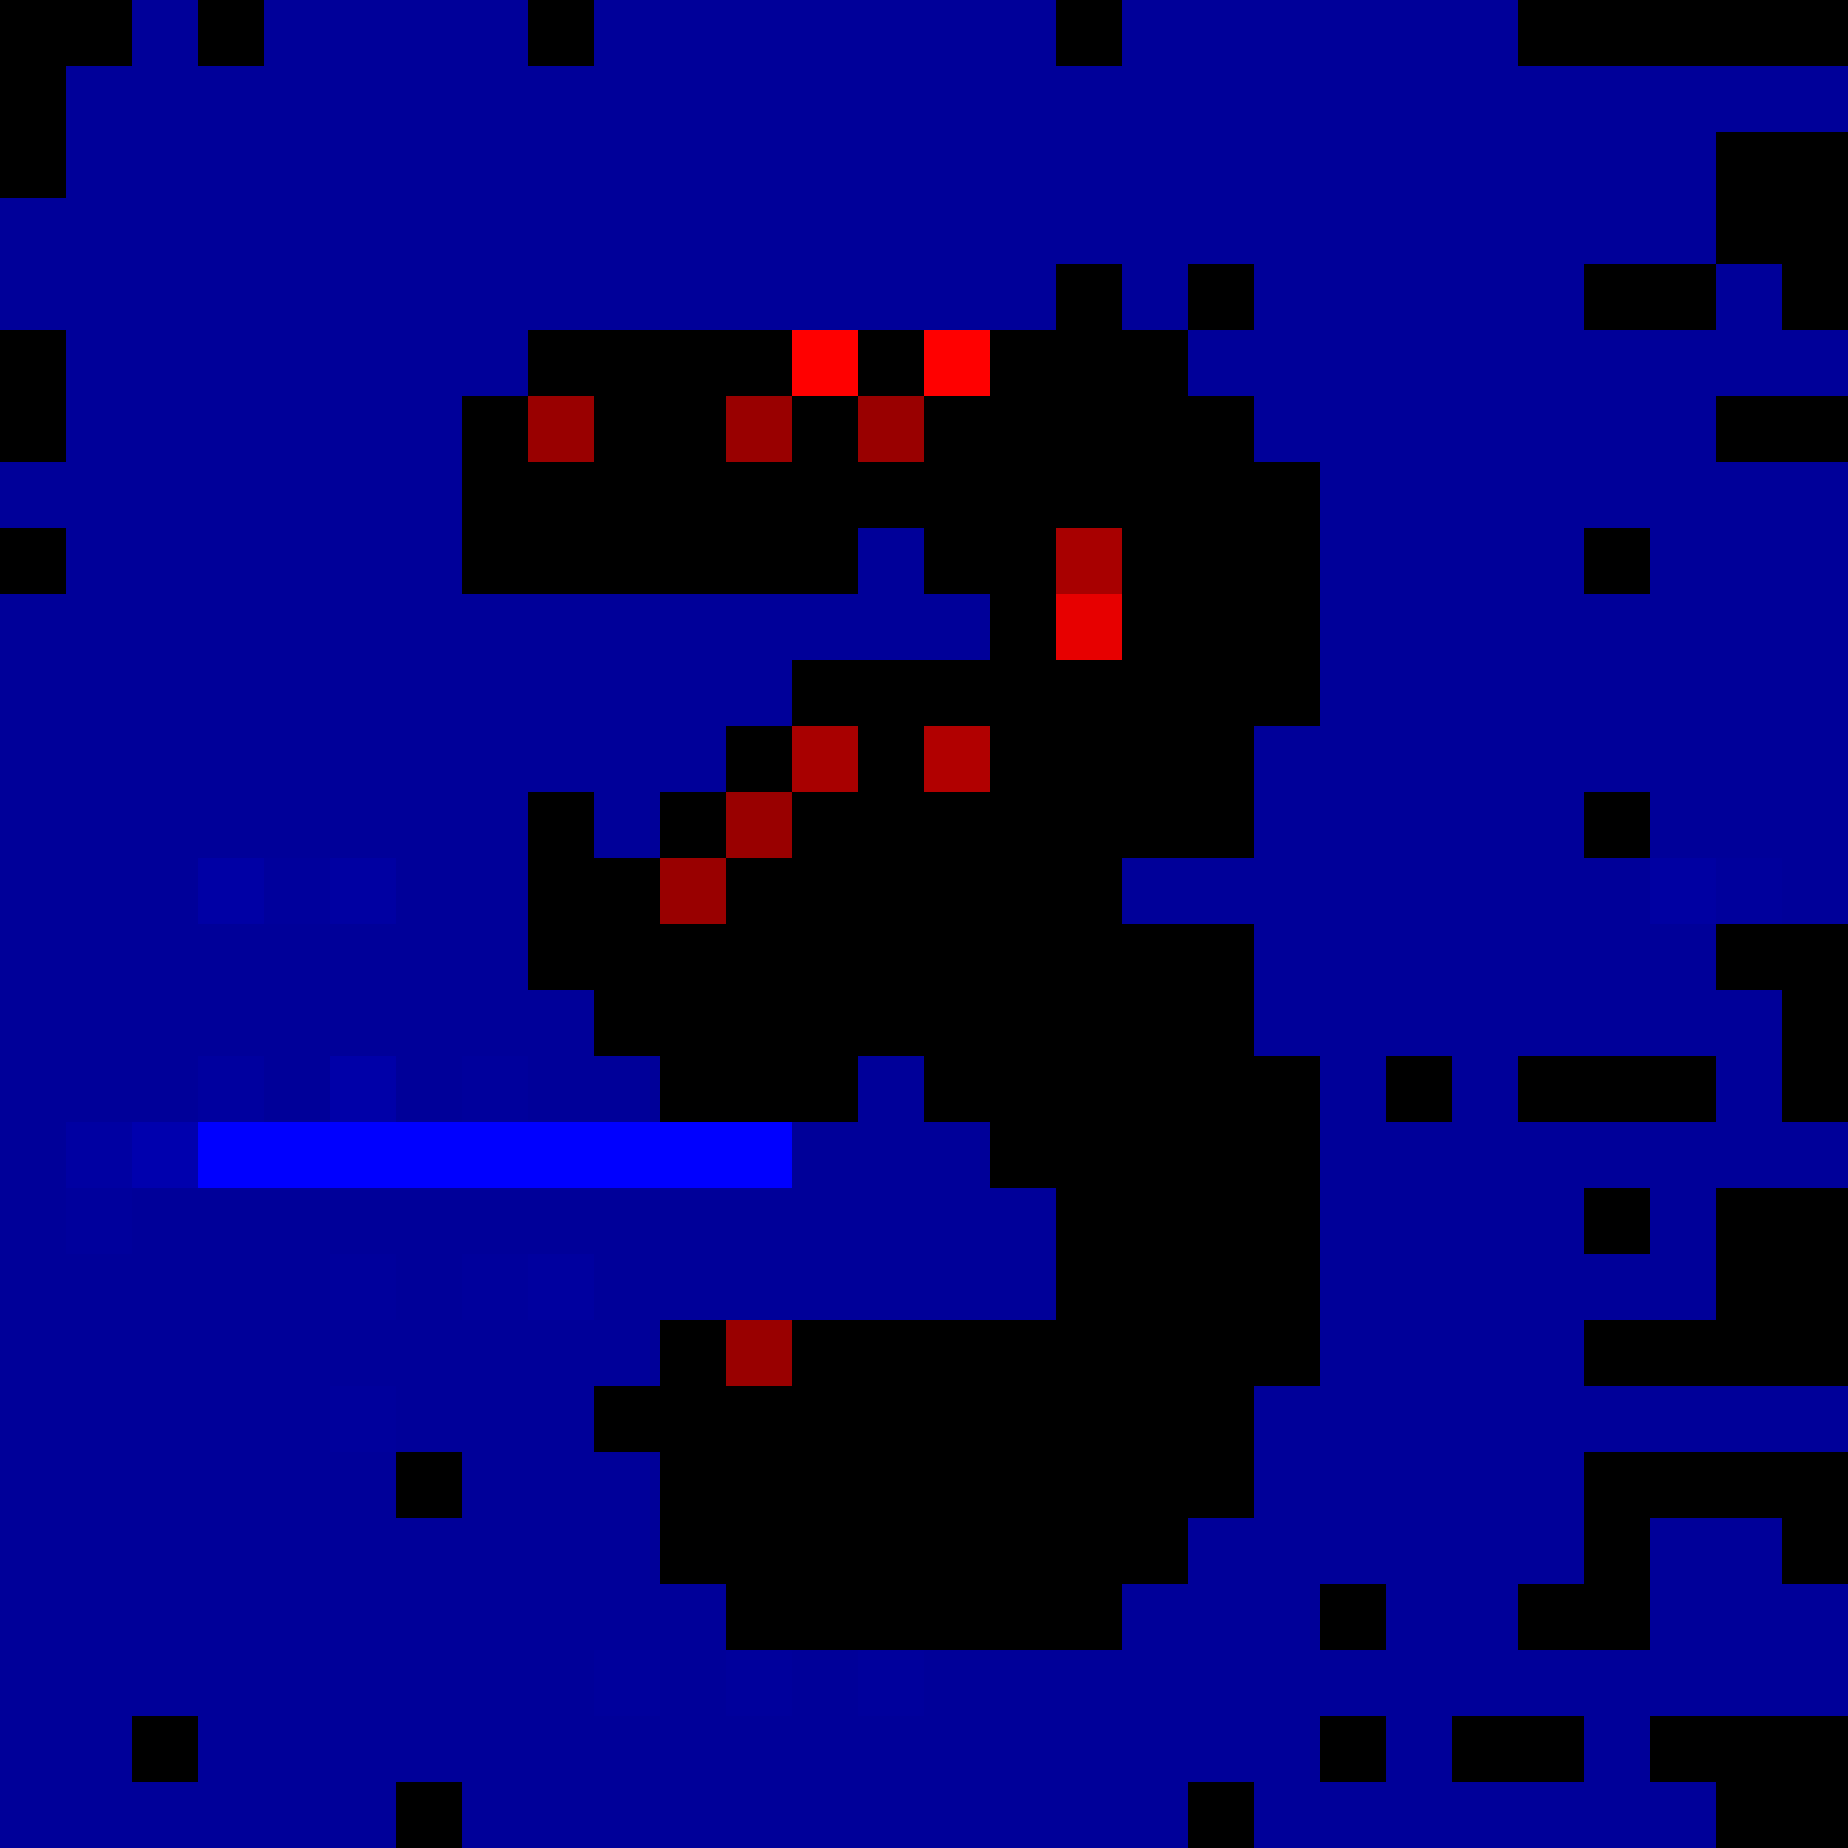
\includegraphics[width=\linewidth]{saliency/mnist_split_ic_saliency/image_036_true_3_pred_3/final_saliency_threshold_wrt_0_bright.png}\\[-1pt]{\scriptsize Logit 0}
		\end{minipage}%
		\begin{minipage}[b]{0.19\linewidth}\centering
			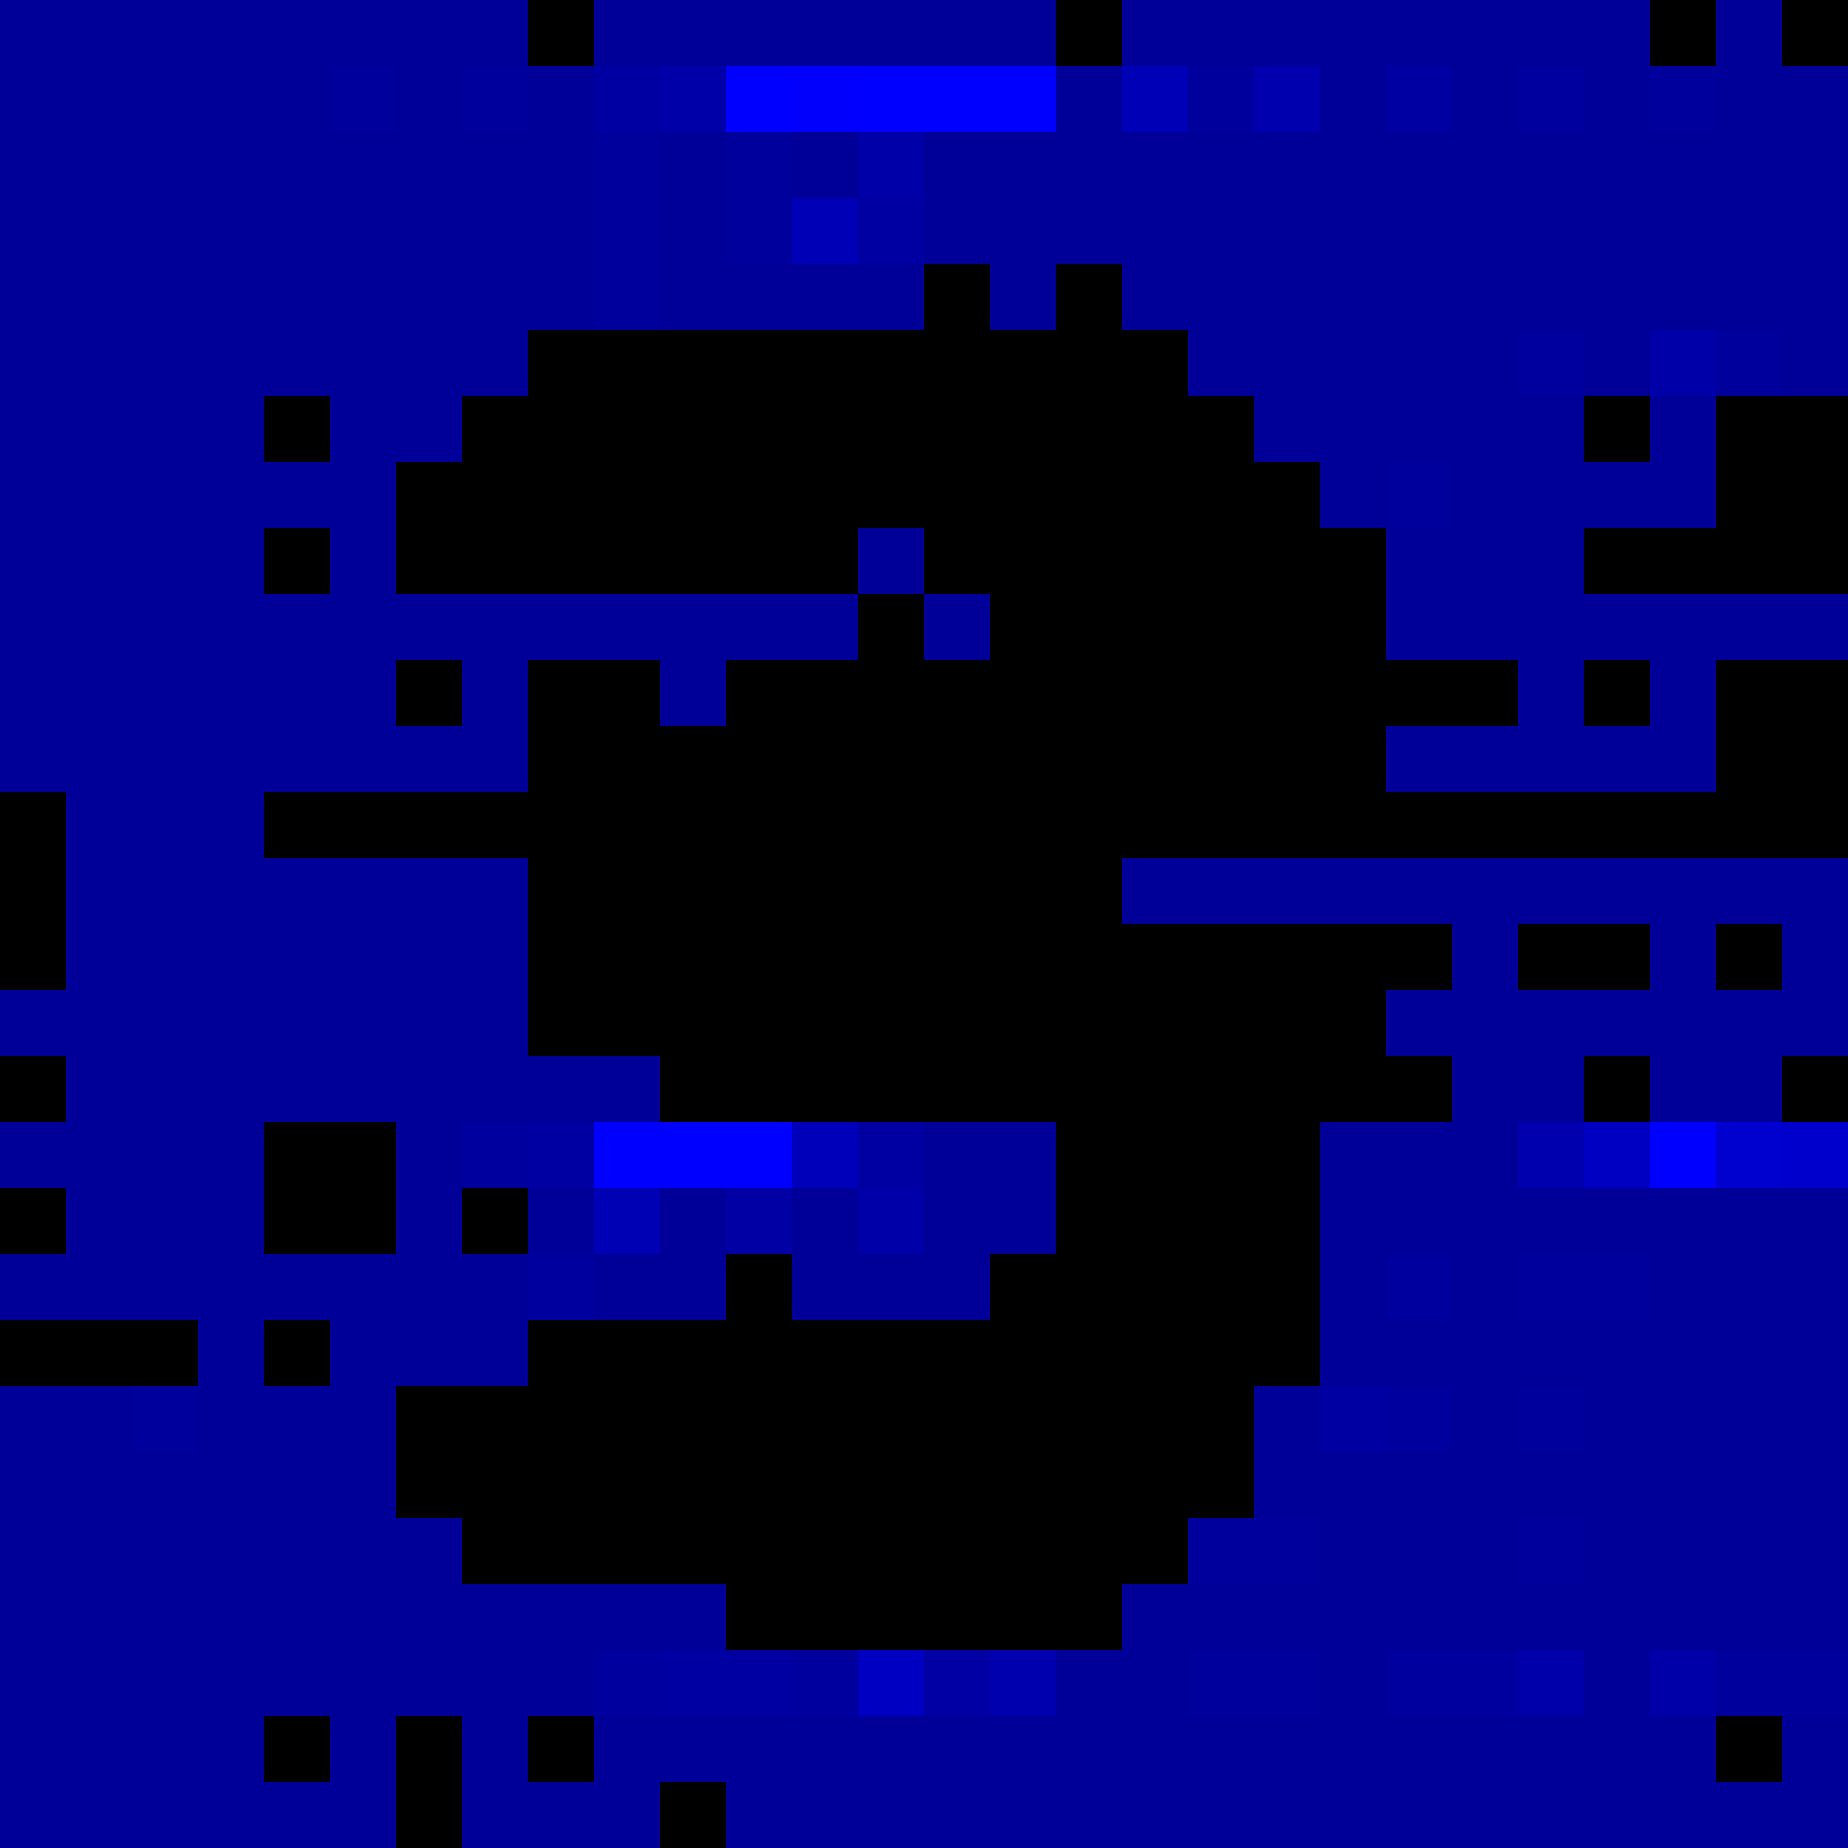
\includegraphics[width=\linewidth]{saliency/mnist_split_ic_saliency/image_036_true_3_pred_3/final_saliency_threshold_wrt_1_bright.png}\\[-1pt]{\scriptsize Logit 1}
		\end{minipage}%
		\begin{minipage}[b]{0.19\linewidth}\centering
			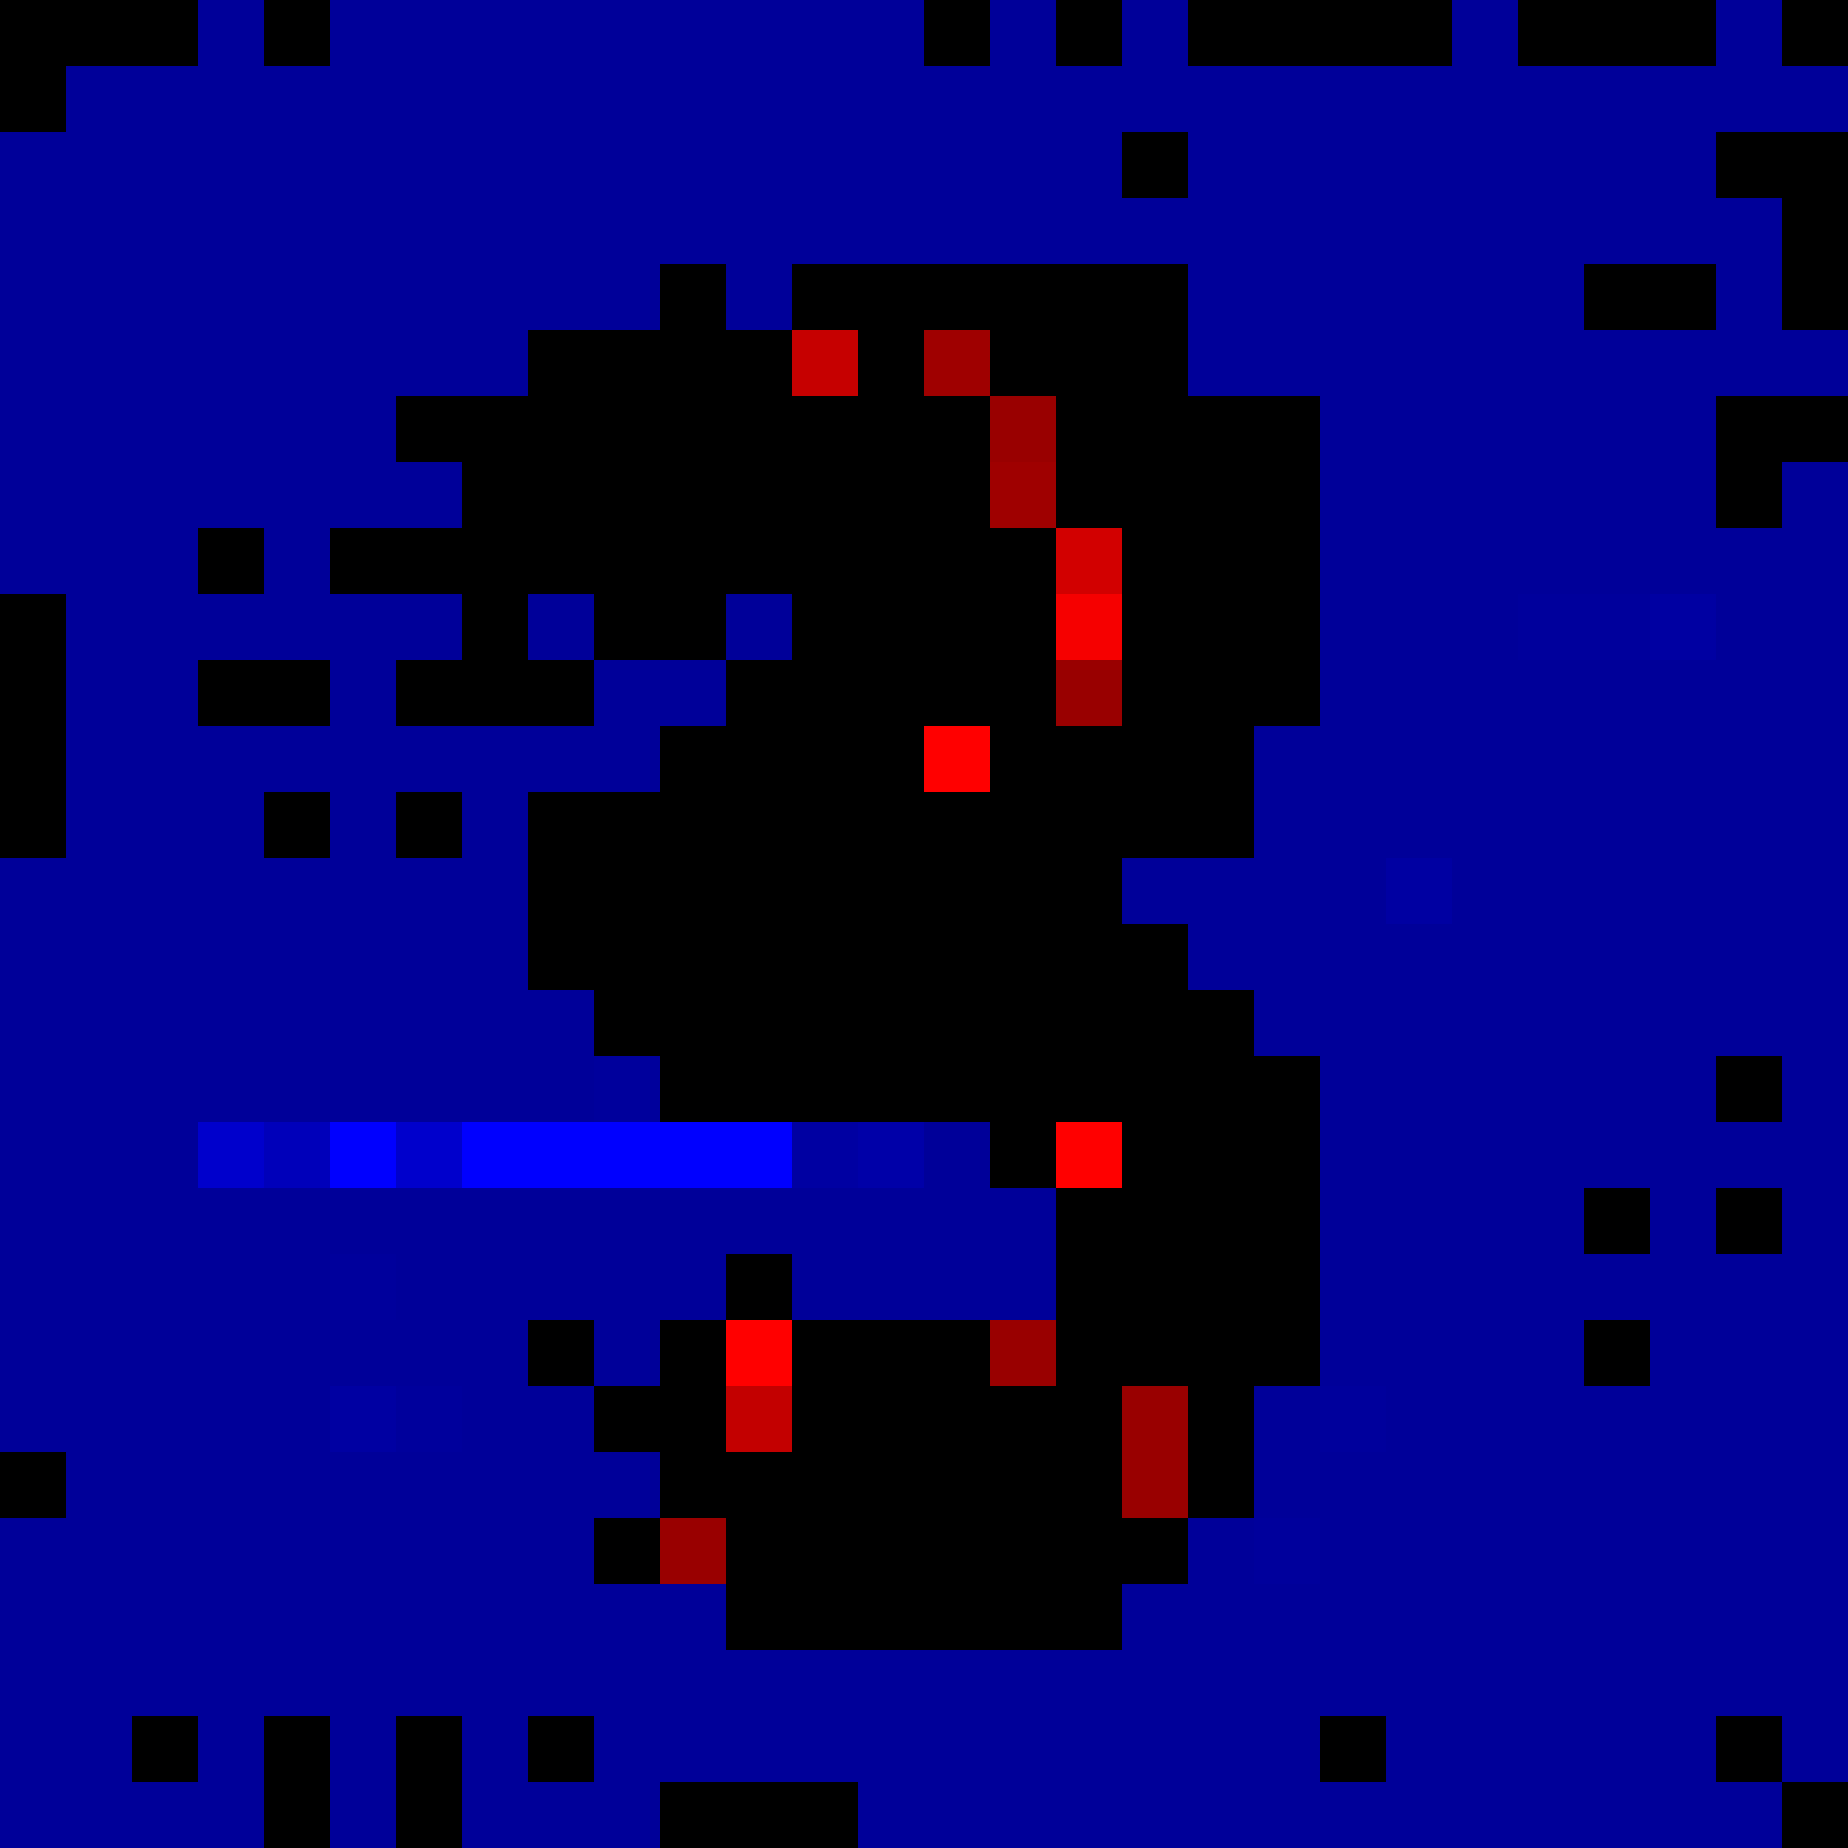
\includegraphics[width=\linewidth]{saliency/mnist_split_ic_saliency/image_036_true_3_pred_3/final_saliency_threshold_wrt_2_bright.png}\\[-1pt]{\scriptsize Logit 2}
		\end{minipage}%
		\begin{minipage}[b]{0.19\linewidth}\centering
			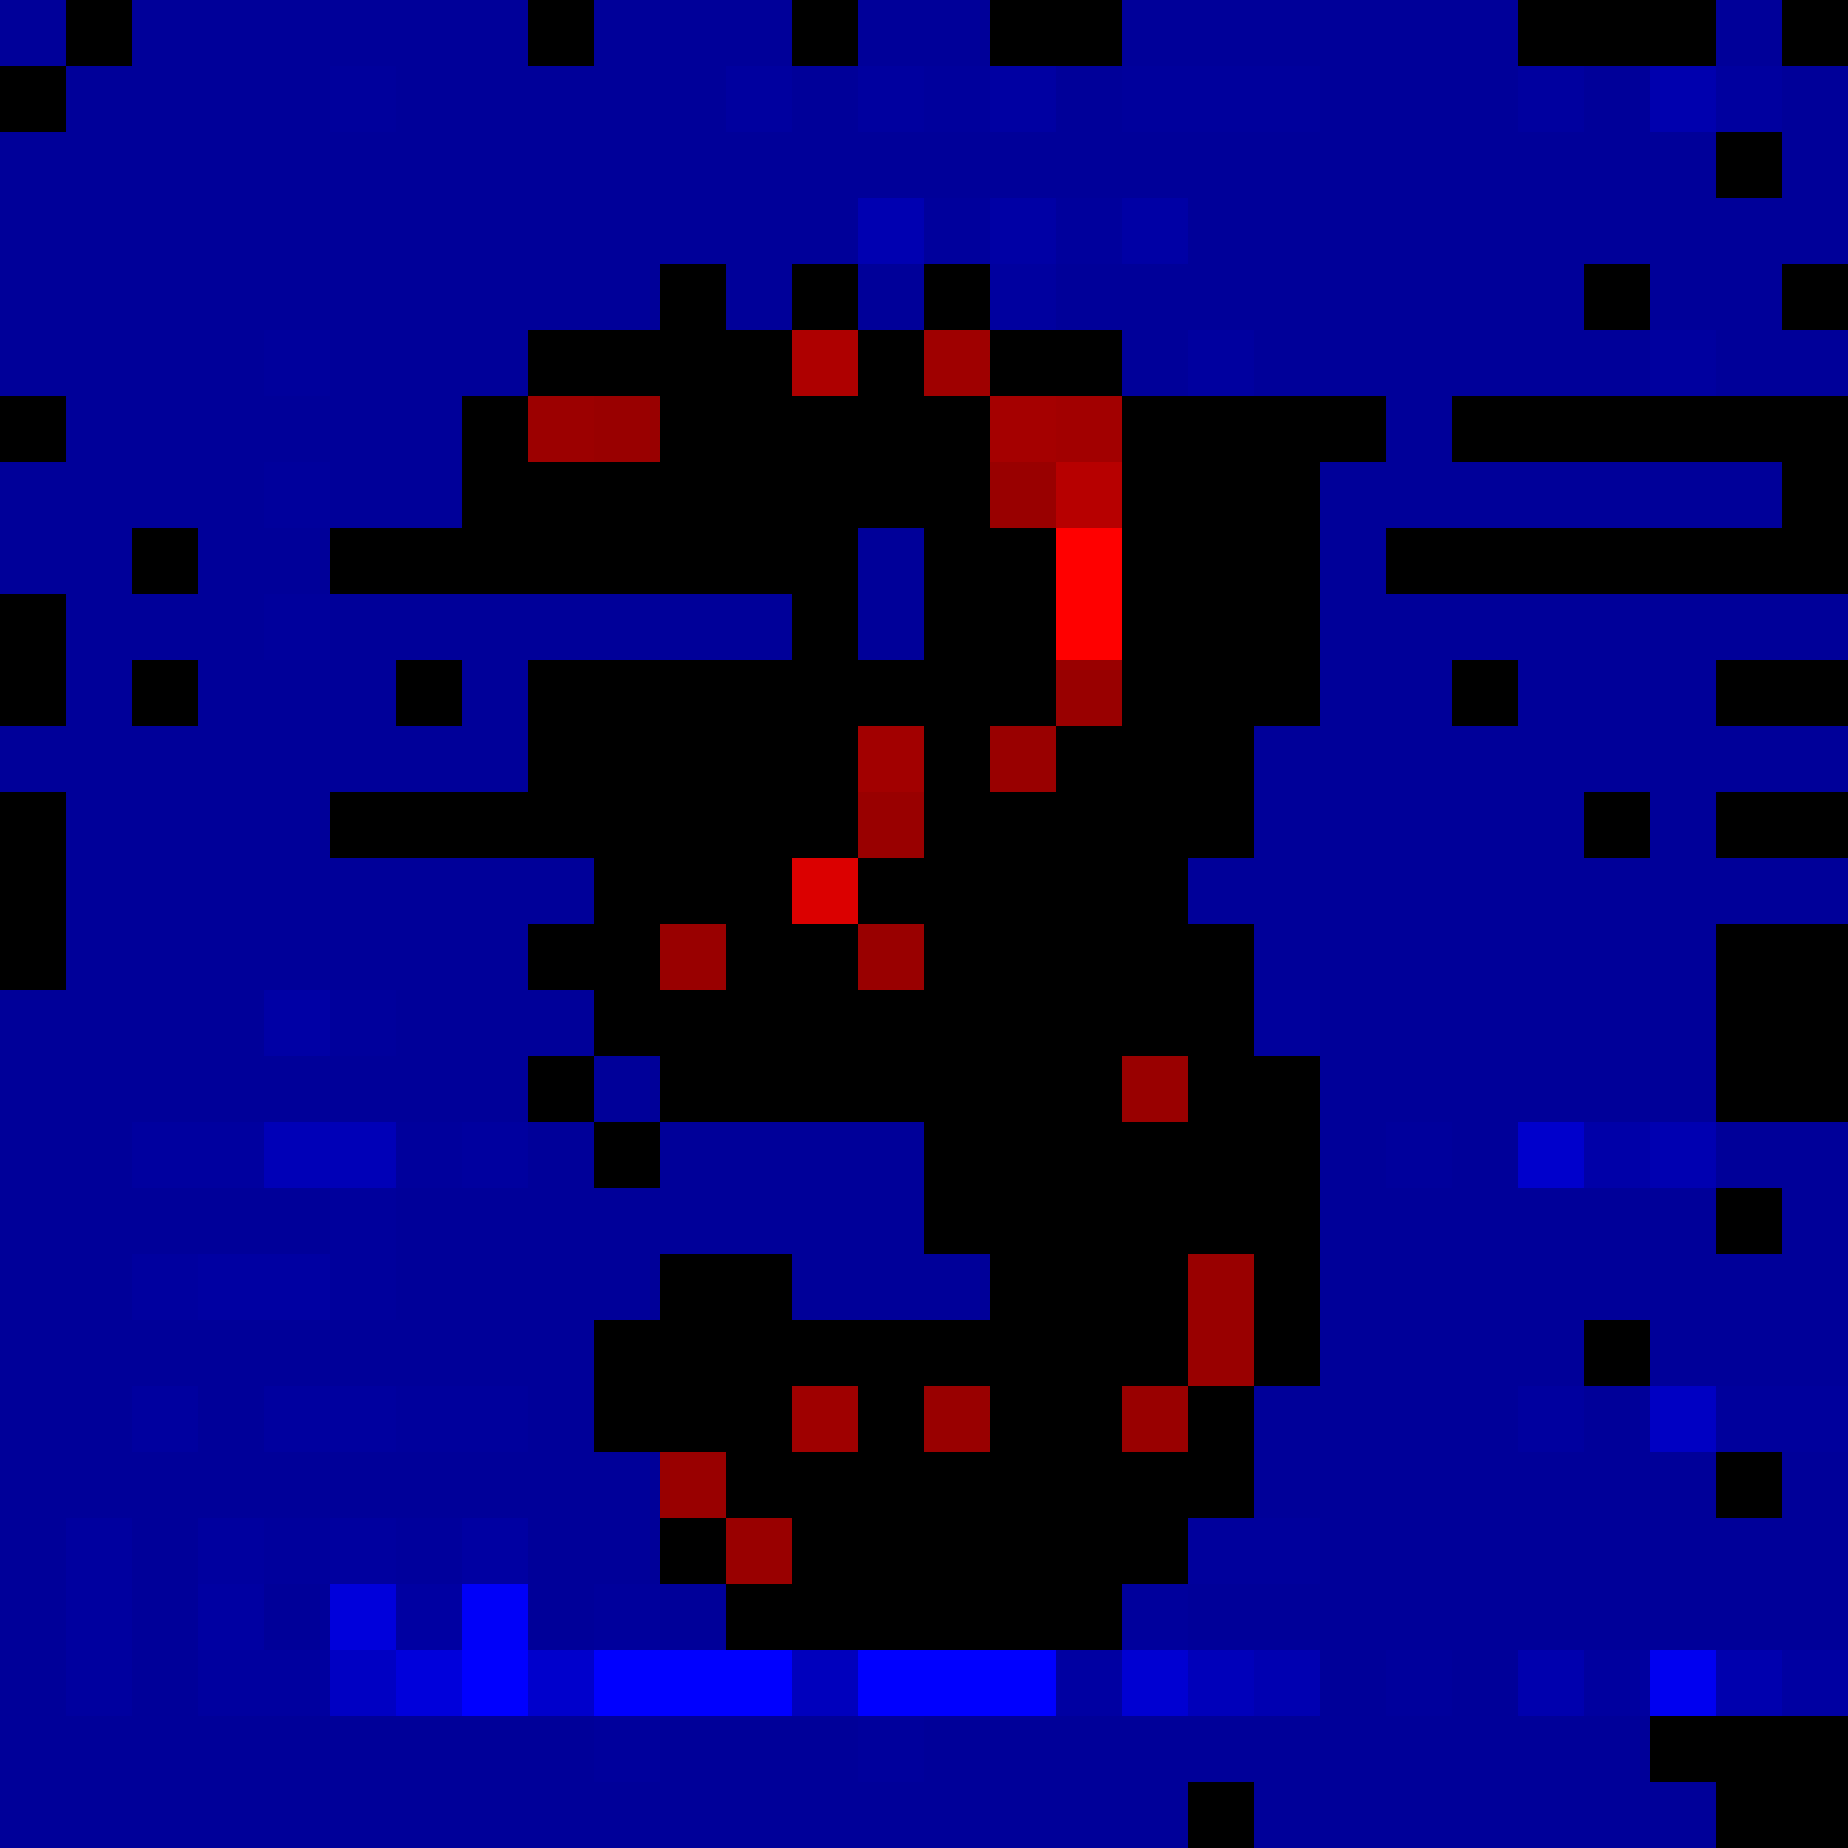
\includegraphics[width=\linewidth]{saliency/mnist_split_ic_saliency/image_036_true_3_pred_3/final_saliency_threshold_wrt_3_bright.png}\\[-1pt]{\scriptsize Logit 3}
		\end{minipage}%
		\begin{minipage}[b]{0.19\linewidth}\centering
			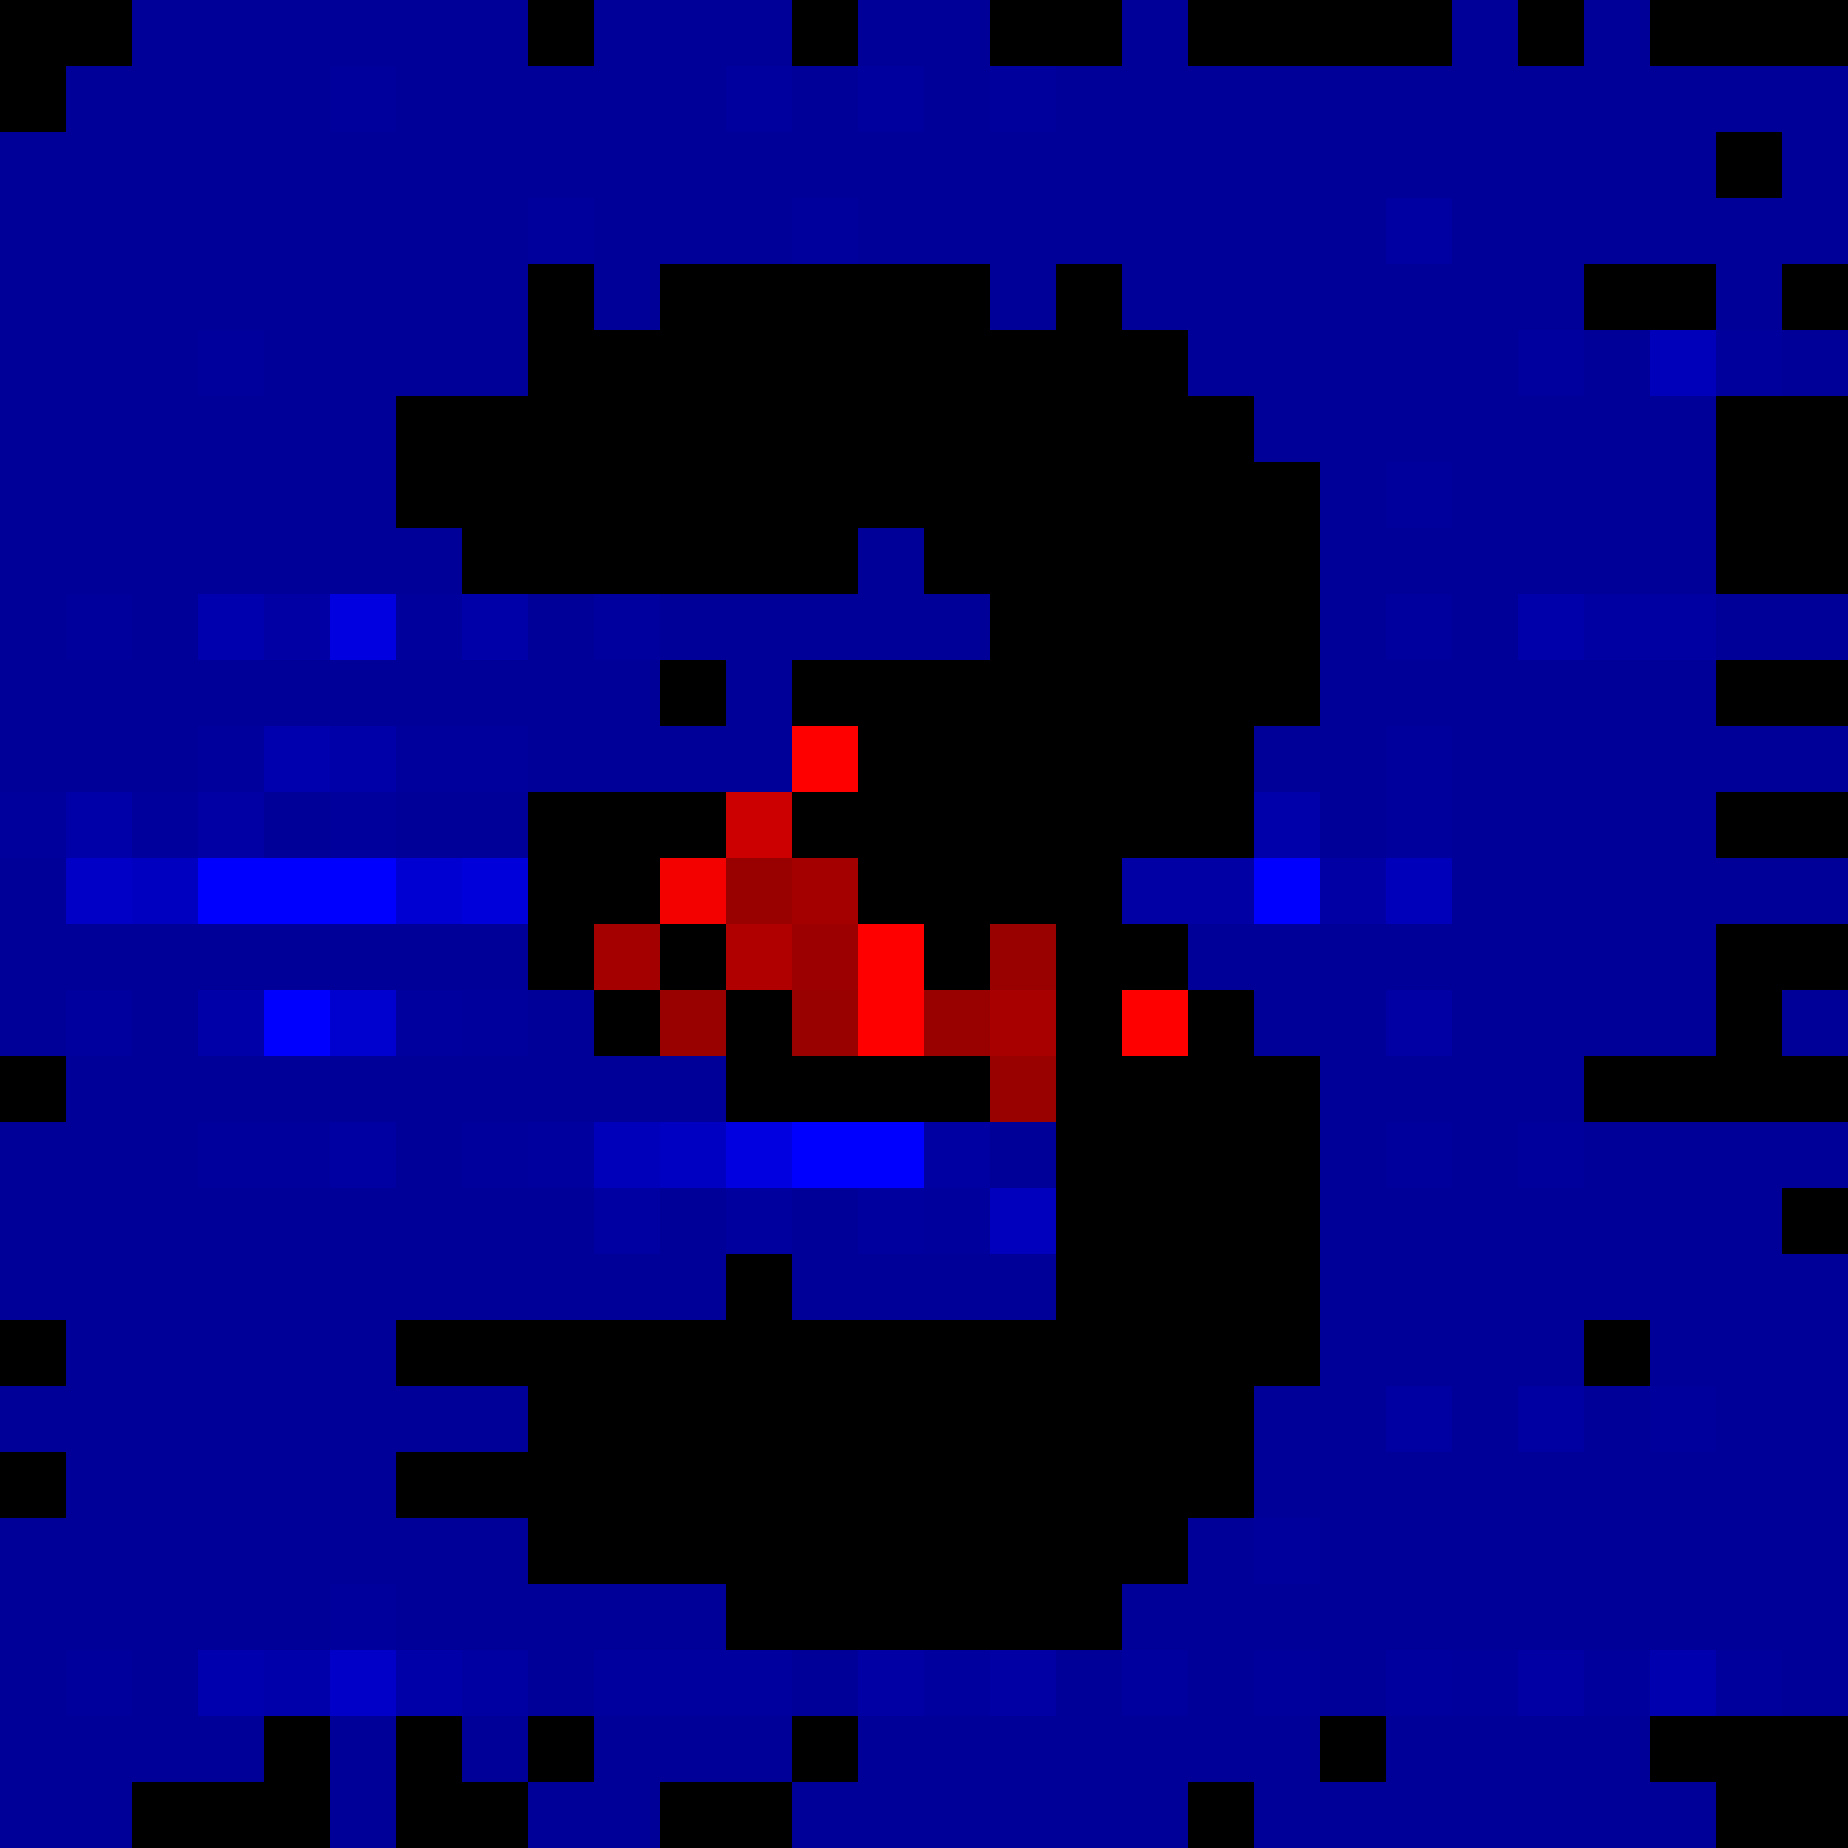
\includegraphics[width=\linewidth]{saliency/mnist_split_ic_saliency/image_036_true_3_pred_3/final_saliency_threshold_wrt_4_bright.png}\\[-1pt]{\scriptsize Logit 4}
		\end{minipage}

		\vspace{0.12cm}

		\begin{minipage}[b]{0.19\linewidth}\centering
			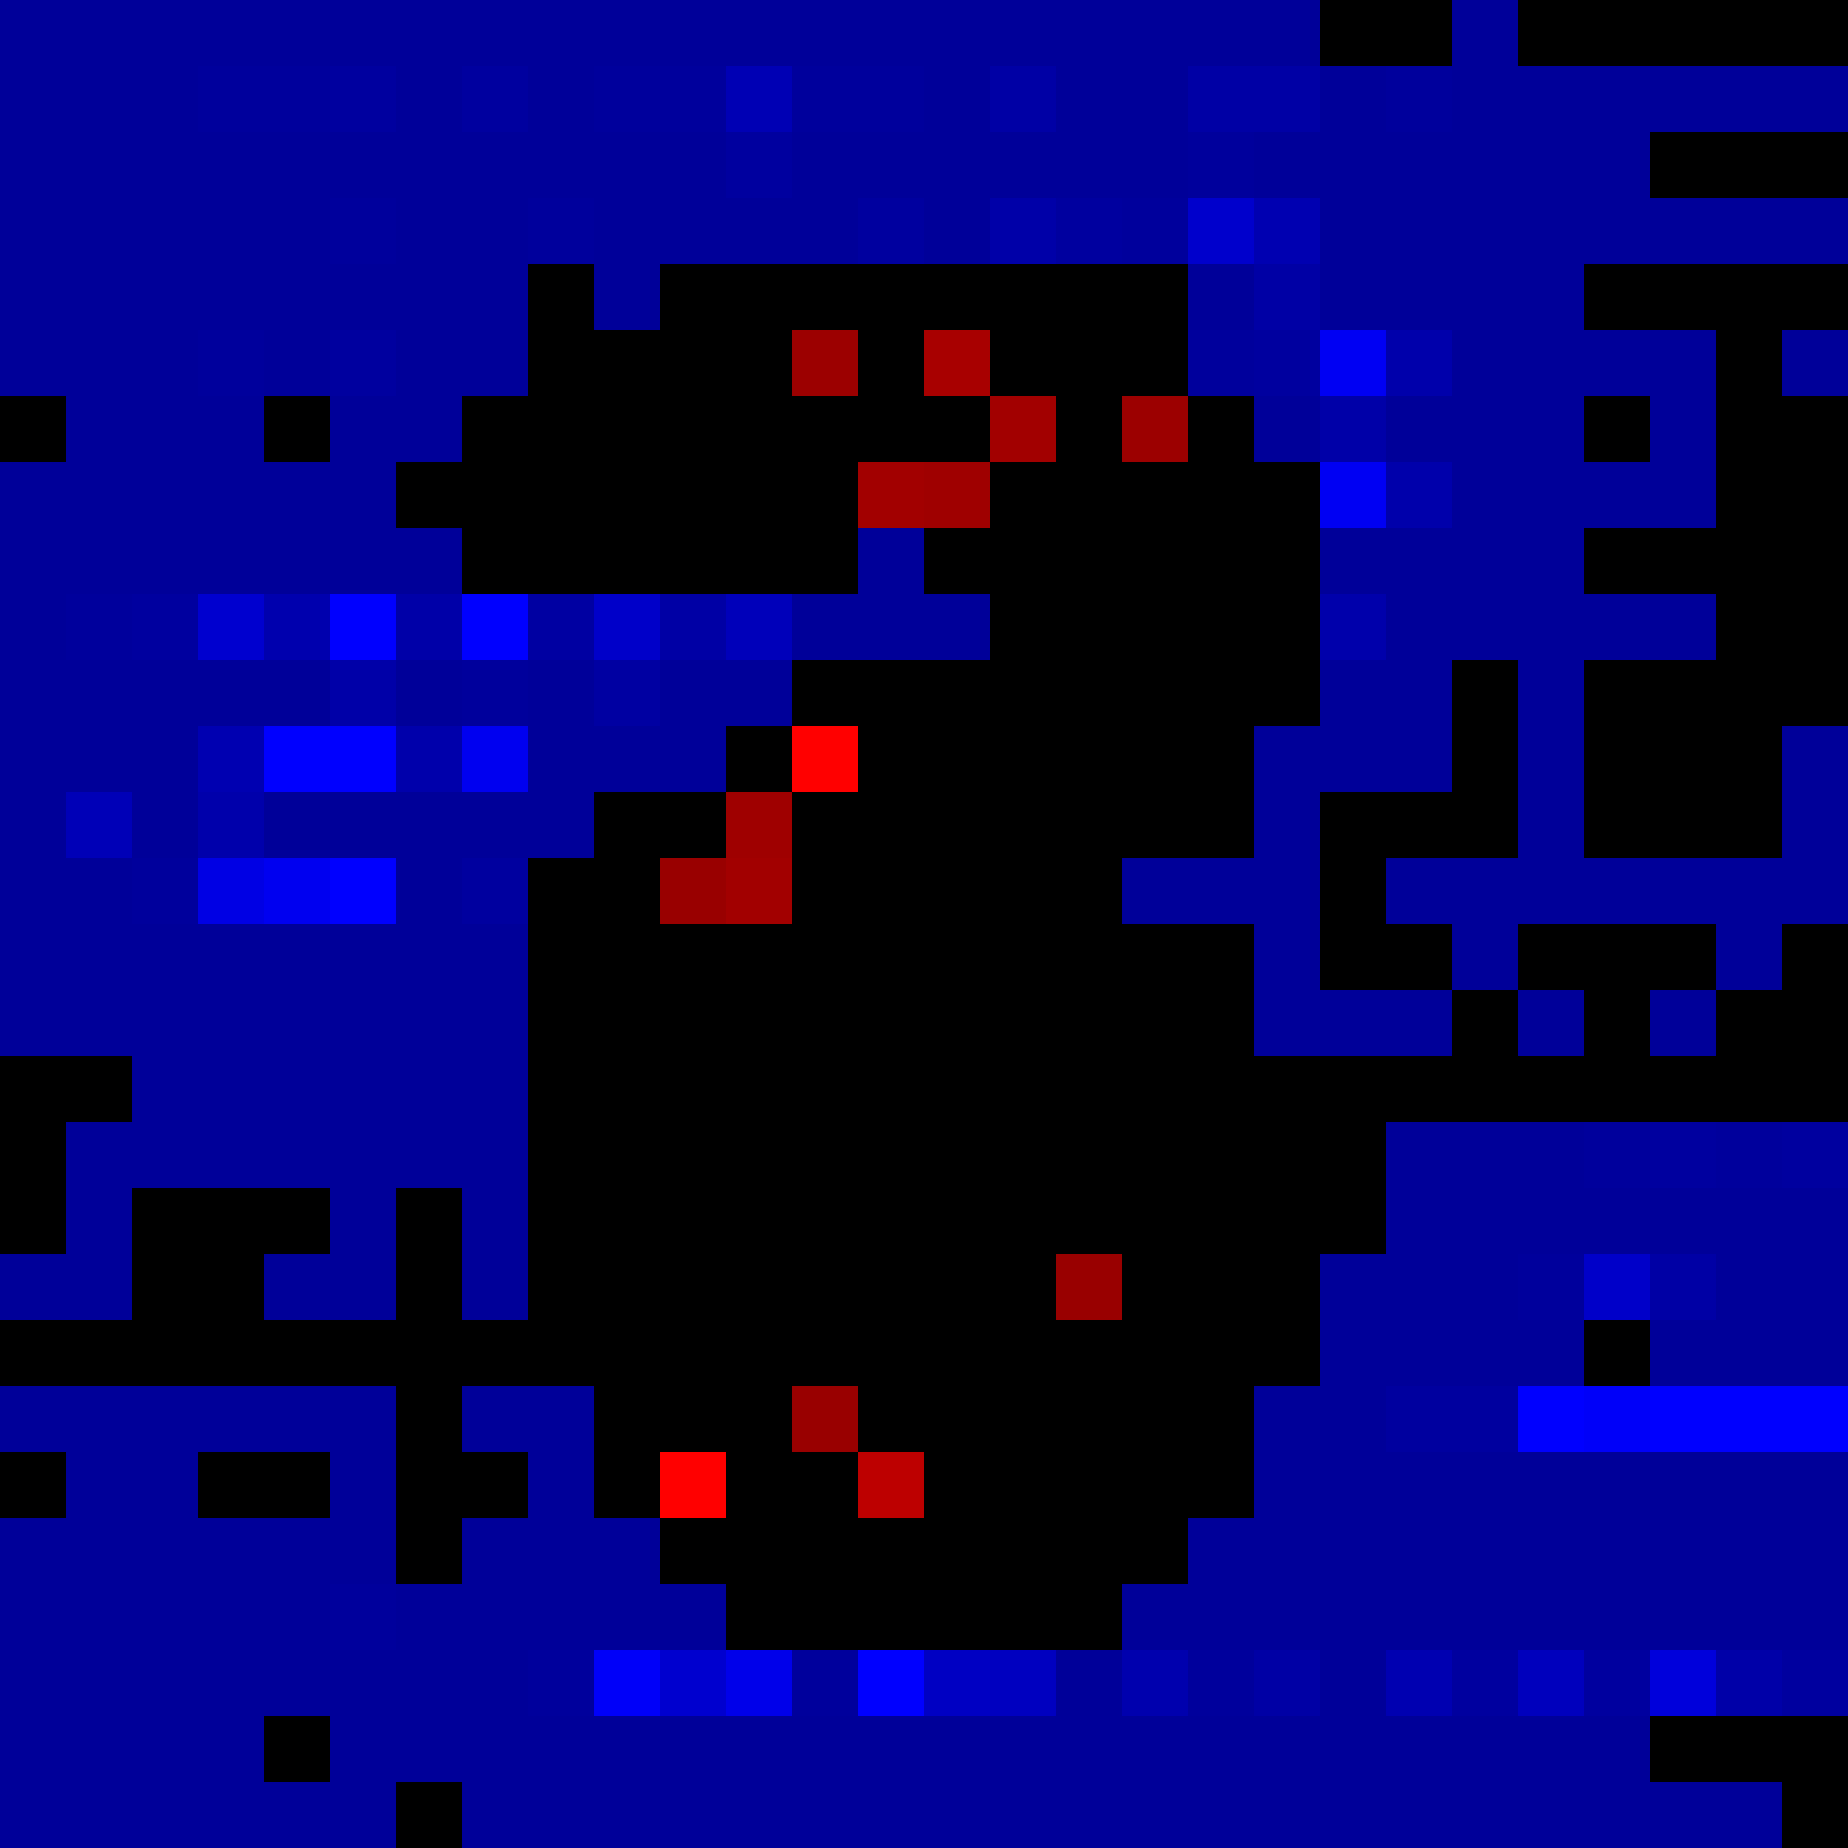
\includegraphics[width=\linewidth]{saliency/mnist_split_ic_saliency/image_036_true_3_pred_3/final_saliency_threshold_wrt_5_bright.png}\\[-1pt]{\scriptsize Logit 5}
		\end{minipage}%
		\begin{minipage}[b]{0.19\linewidth}\centering
			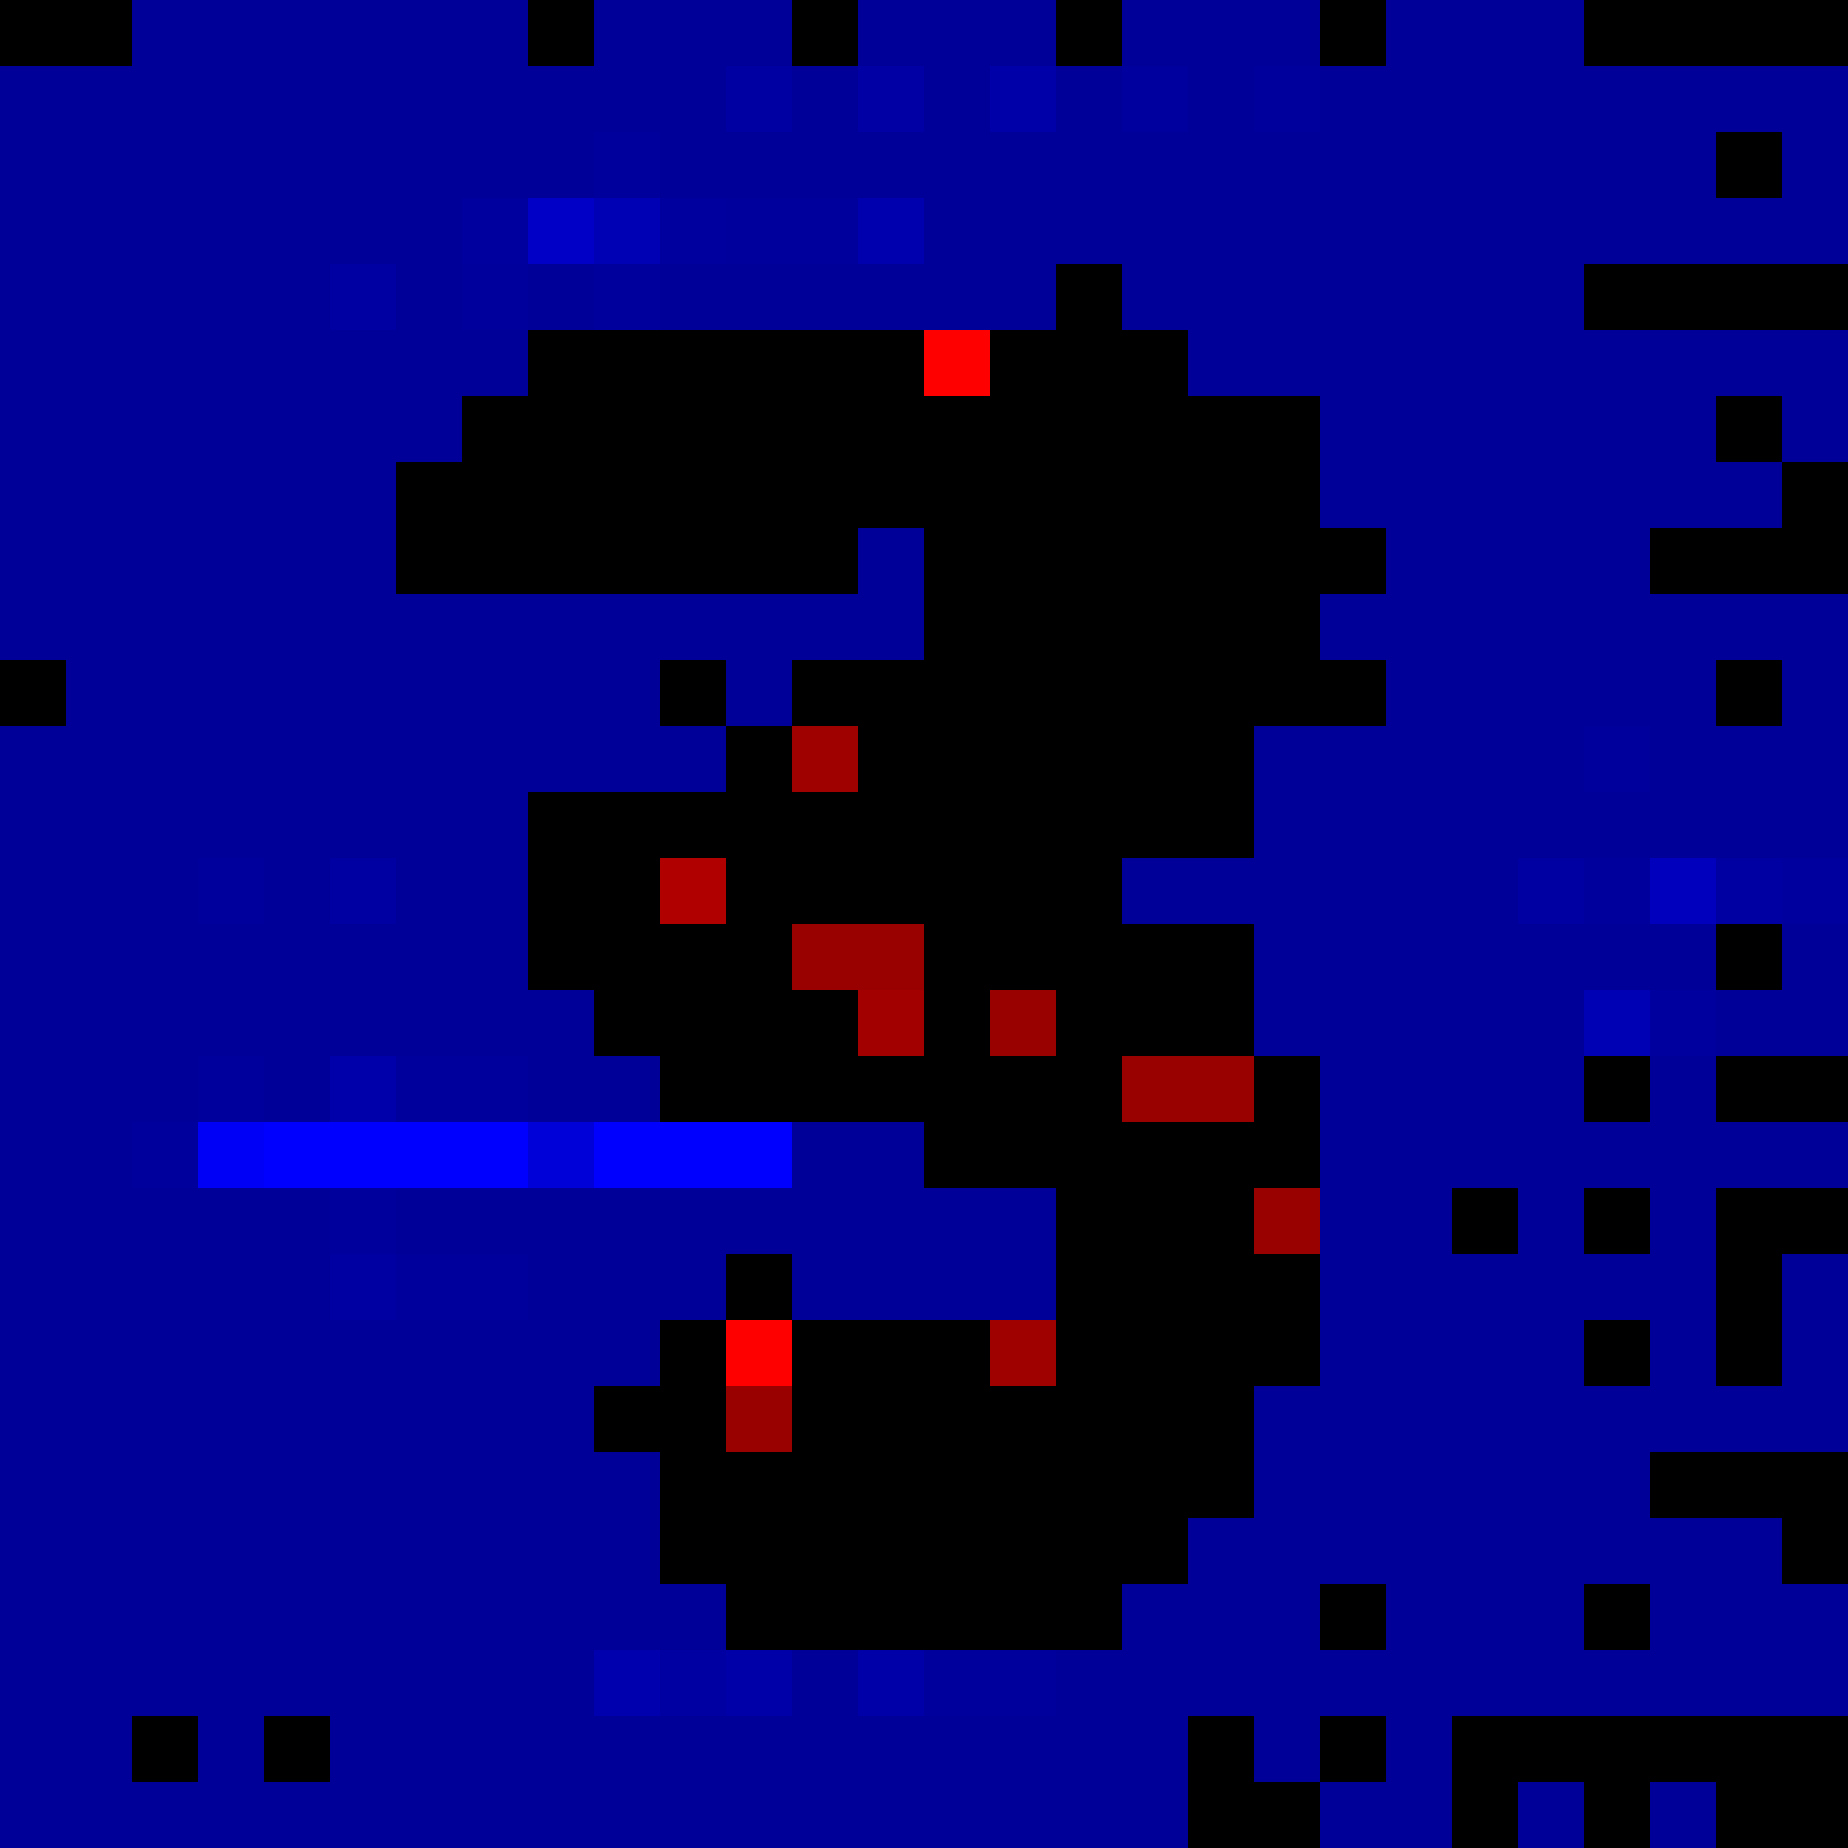
\includegraphics[width=\linewidth]{saliency/mnist_split_ic_saliency/image_036_true_3_pred_3/final_saliency_threshold_wrt_6_bright.png}\\[-1pt]{\scriptsize Logit 6}
		\end{minipage}%
		\begin{minipage}[b]{0.19\linewidth}\centering
			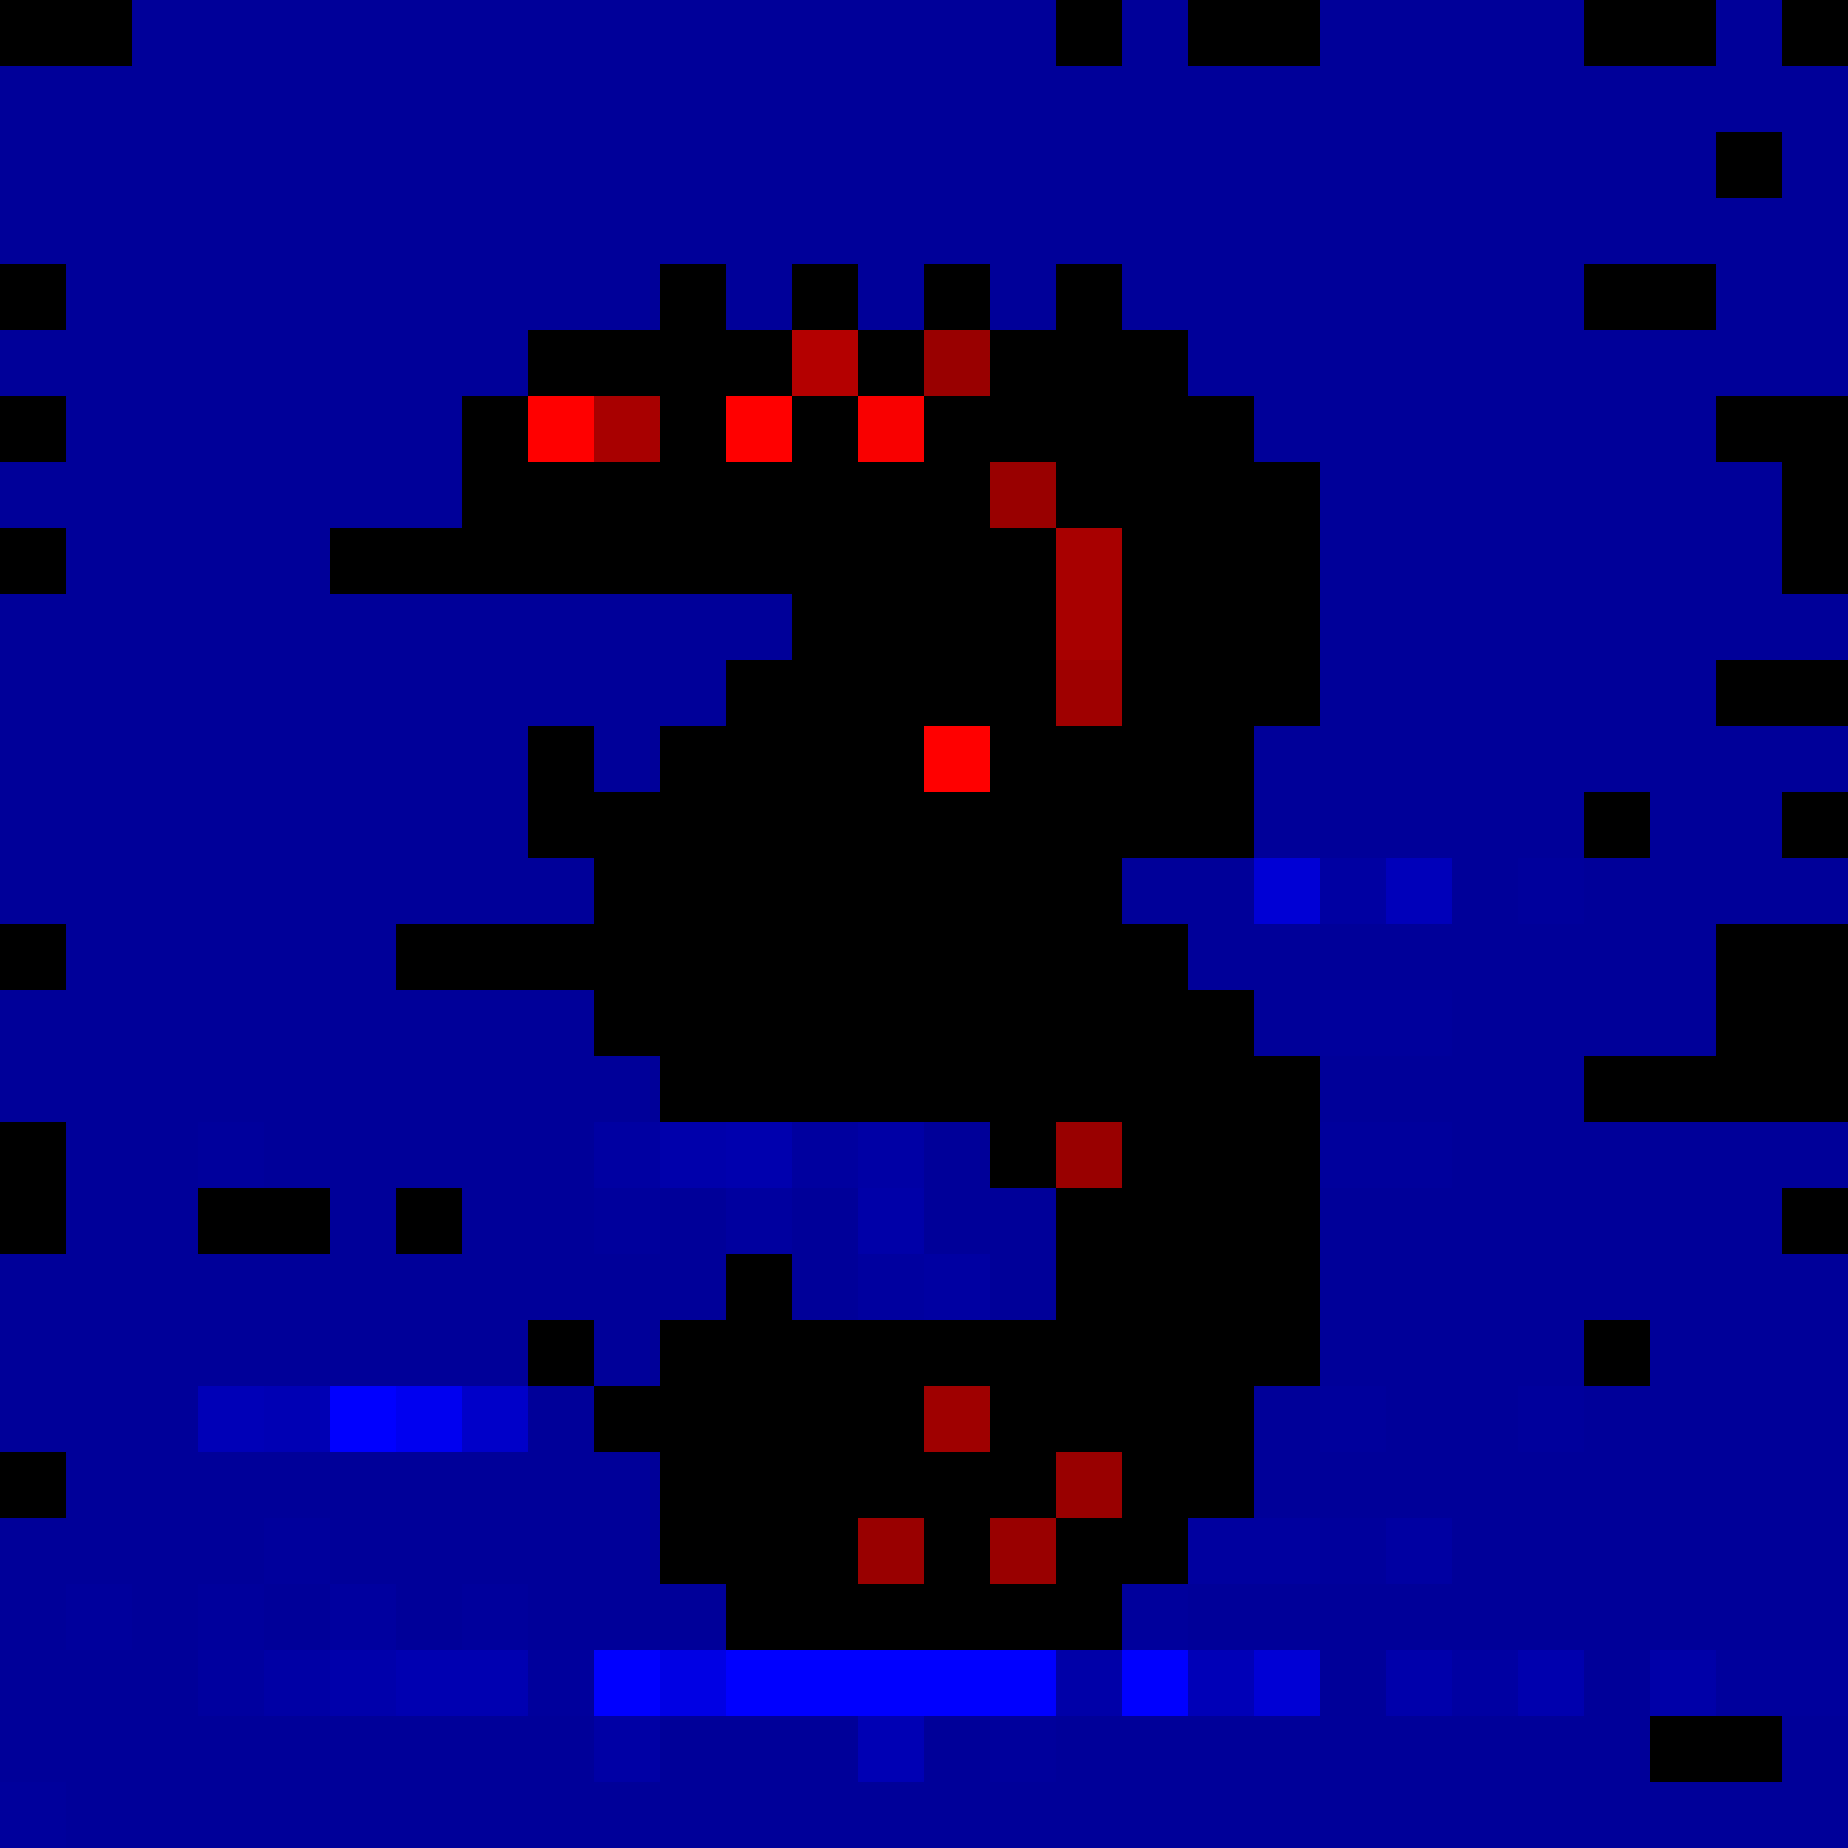
\includegraphics[width=\linewidth]{saliency/mnist_split_ic_saliency/image_036_true_3_pred_3/final_saliency_threshold_wrt_7_bright.png}\\[-1pt]{\scriptsize Logit 7}
		\end{minipage}%
		\begin{minipage}[b]{0.19\linewidth}\centering
			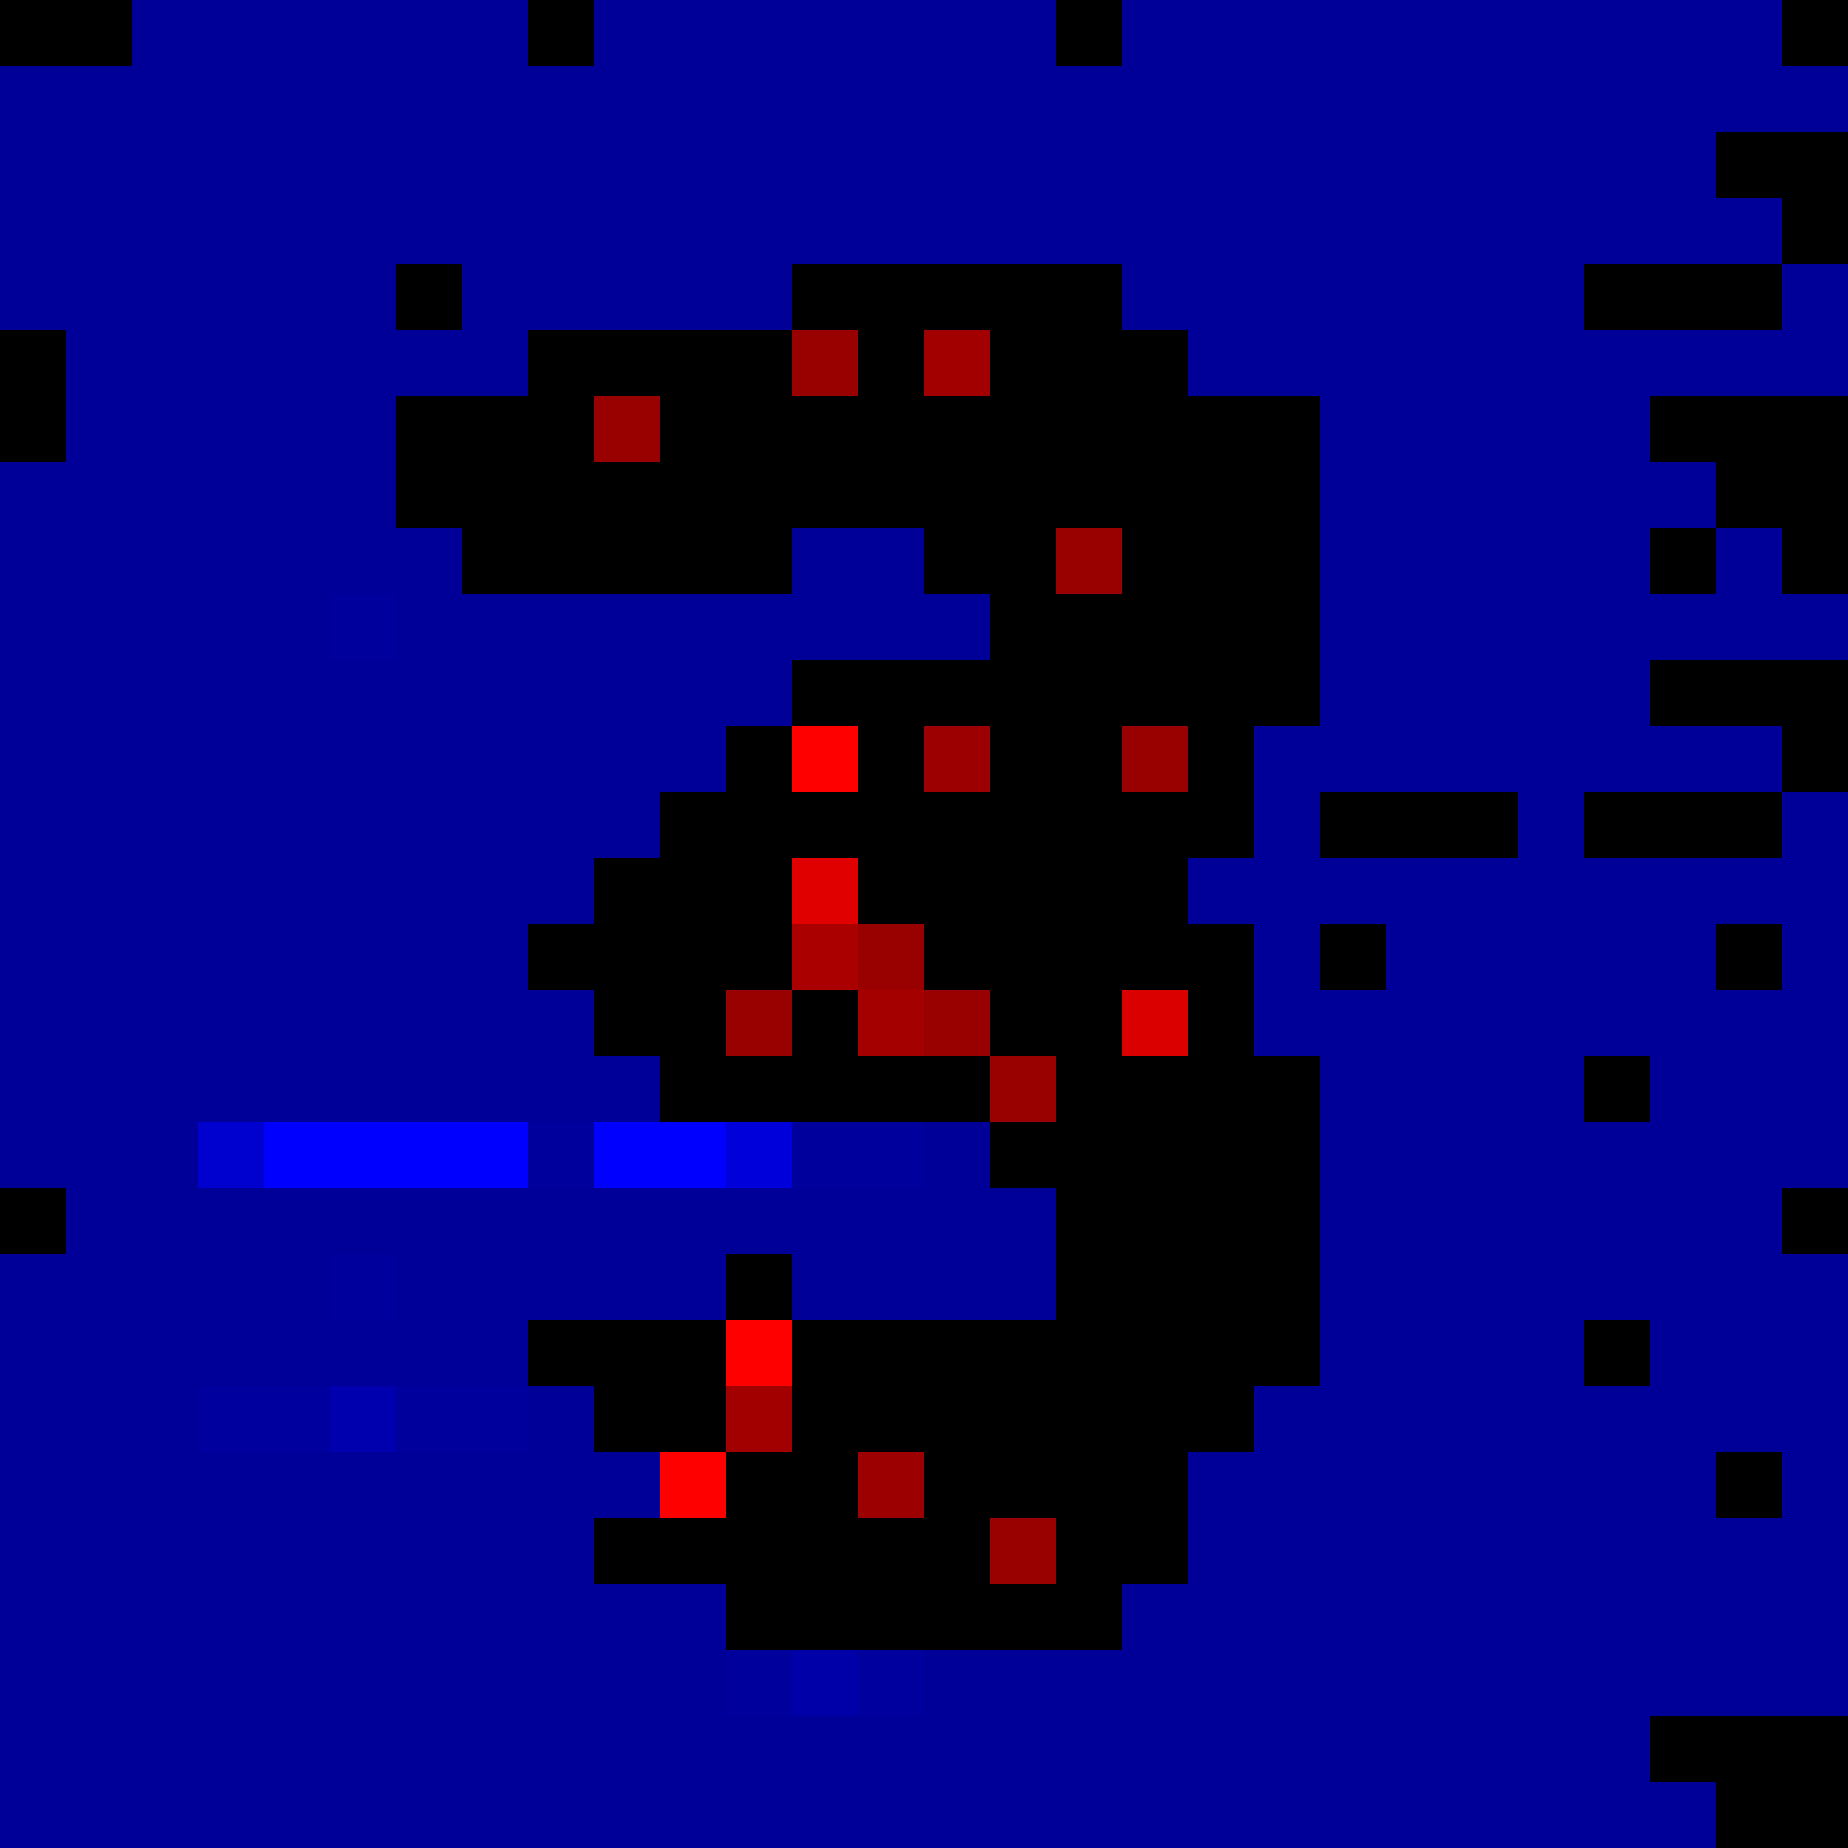
\includegraphics[width=\linewidth]{saliency/mnist_split_ic_saliency/image_036_true_3_pred_3/final_saliency_threshold_wrt_8_bright.png}\\[-1pt]{\scriptsize Logit 8}
		\end{minipage}%
		\begin{minipage}[b]{0.19\linewidth}\centering
			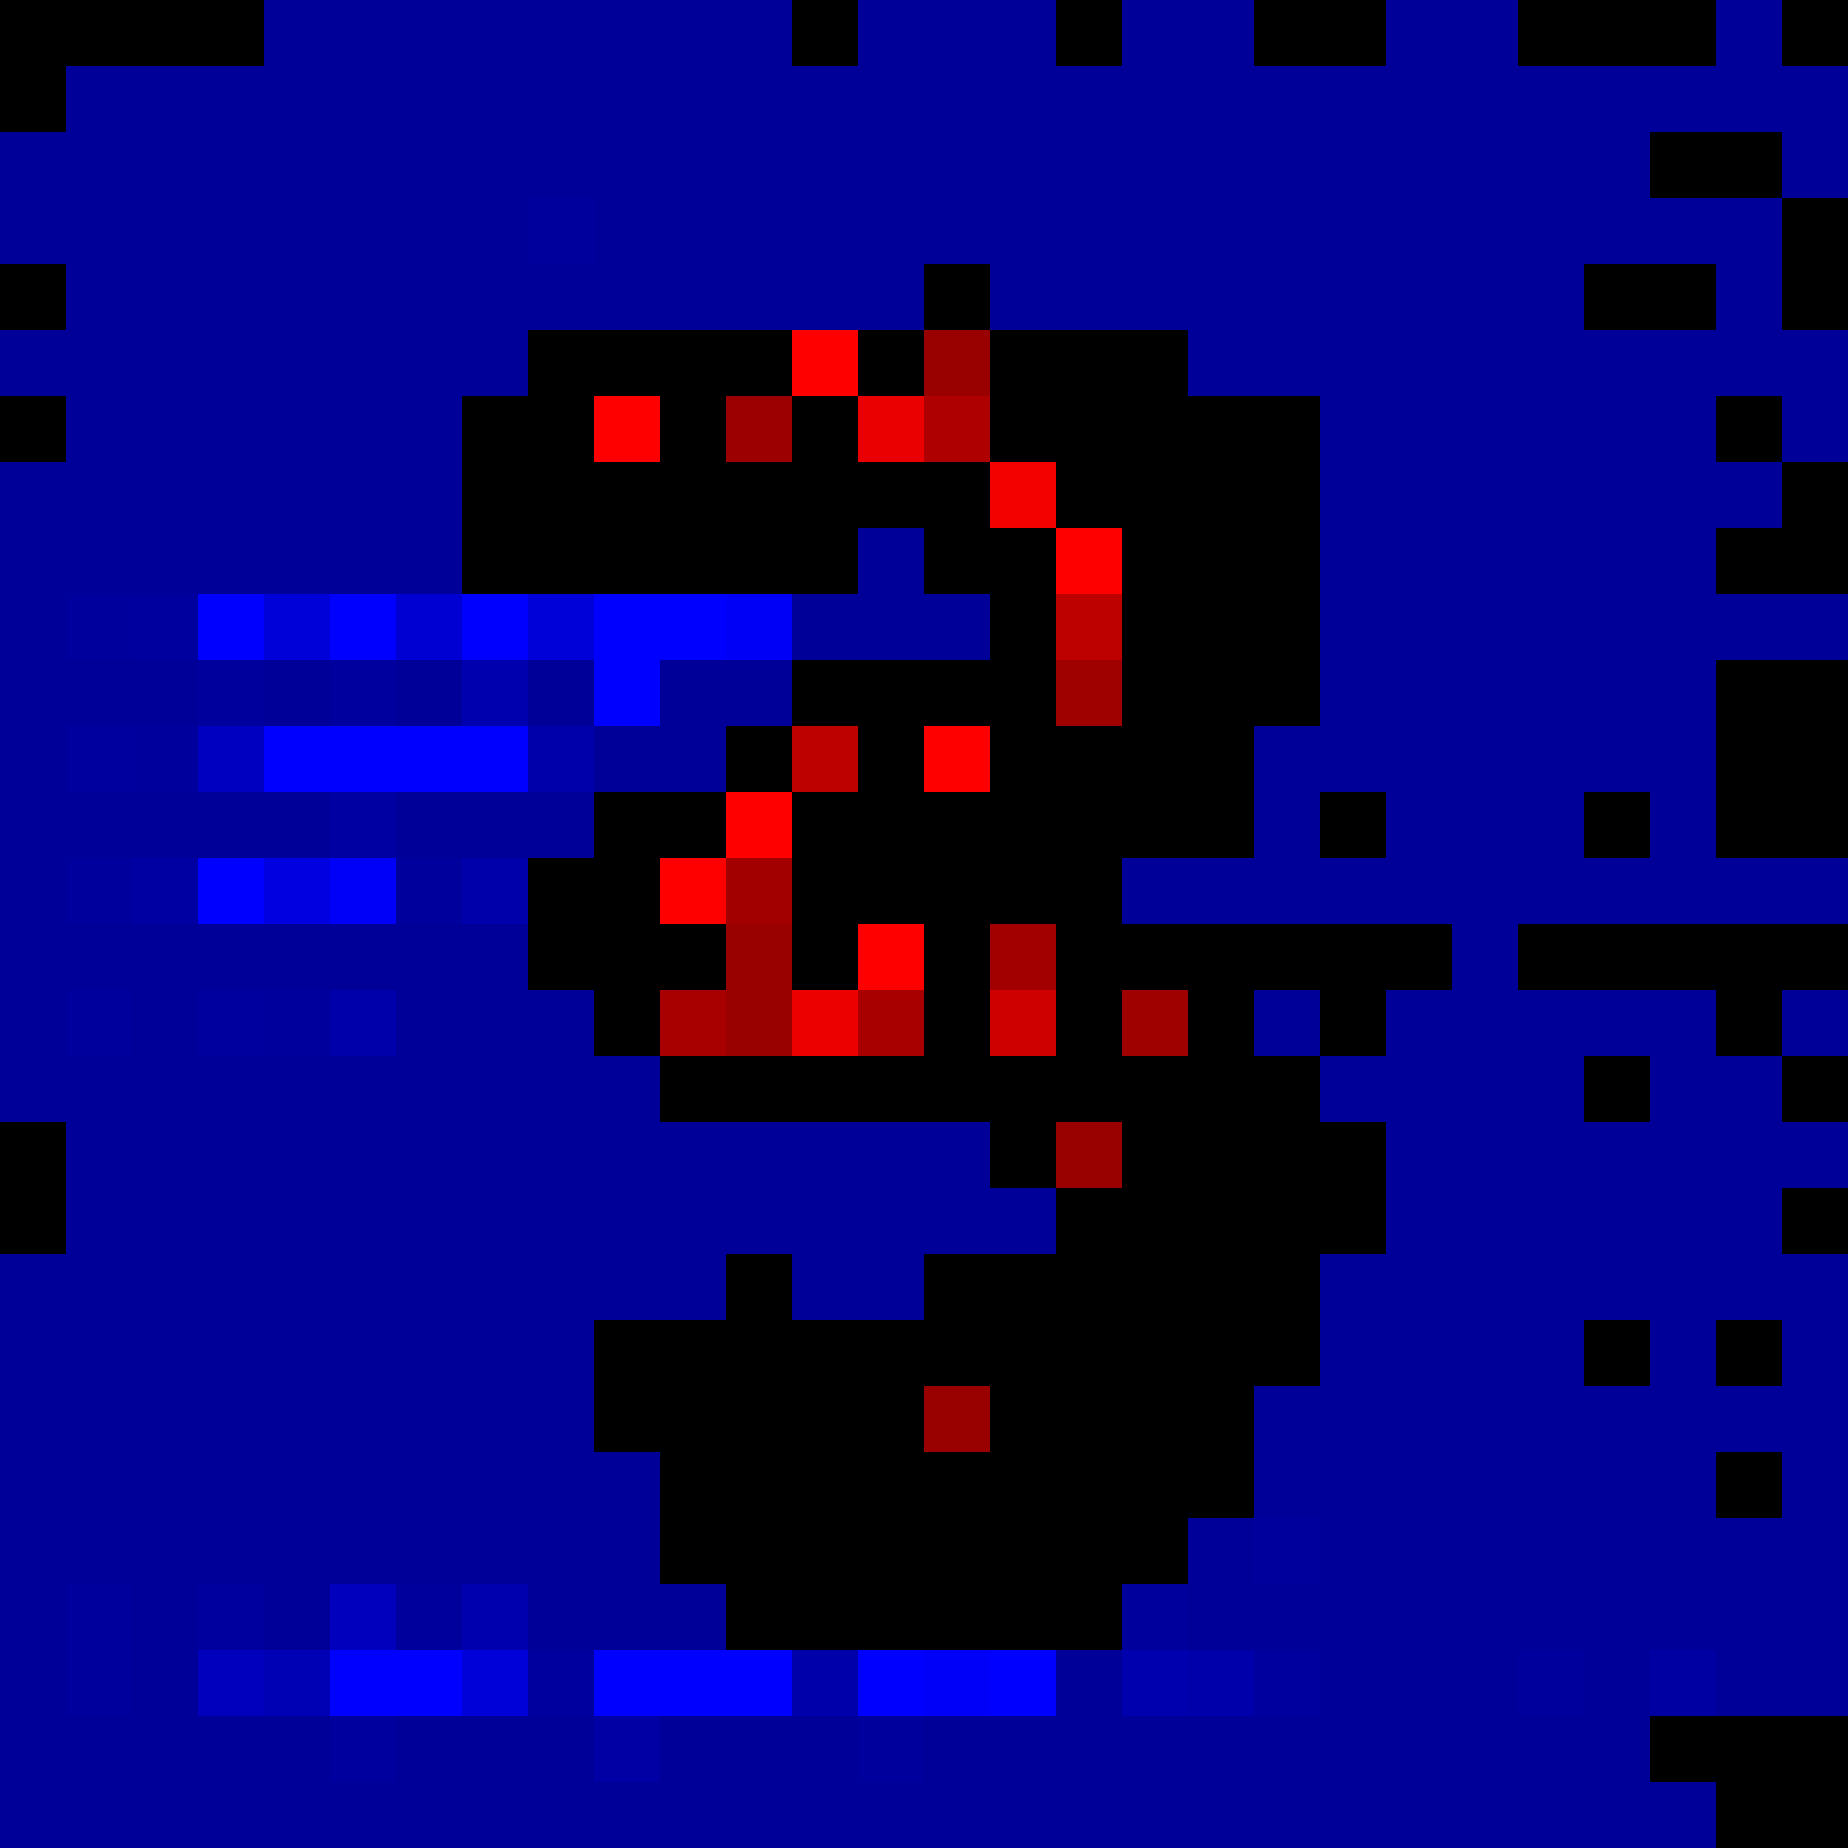
\includegraphics[width=\linewidth]{saliency/mnist_split_ic_saliency/image_036_true_3_pred_3/final_saliency_threshold_wrt_9_bright.png}\\[-1pt]{\scriptsize Logit 9}
		\end{minipage}
	\end{minipage}
	}%
\caption[Second example of inverted-input DIC stream gradients]{Second correctly classified MNIST test ``3'', using the model, per-class thresholded overlays and color convention of Figure~\ref{fig:mnist_split_ic_saliency}. Left: input.}
	\label{fig:mnist_split_ic_saliency_second}
\end{figure}

Figure~\ref{fig:mnist_split_ic_saliency} overlays both gradients for each class logit of a test ``3''. The $g$-gradient for the ground-truth class ``3'' follows the digit strokes most accurately. For classes ``6'', ``8'' and ``9'', the $h$-gradients are dense \emph{between the arches} of the ``3'', at candidate missing-stroke locations that would geometrically close loops. A second correctly classified ``3'' (Figure~\ref{fig:mnist_split_ic_saliency_second}) shows the same qualitative pattern. The gradients of the single \texttt{cnn\_maxout} IC model are mostly positive on the strokes and negative on the background, with less class-dependent directional variation. These examples illustrate class-dependent stream sensitivities in the difference model.

Figure~\ref{fig:mnist_ic_saliency} visualizes input gradients of the \texttt{cnn\_maxout} IC model on representative test samples.

\begin{figure}[t]
\QualitativeImageContent{
    \centering
    \begin{minipage}[b]{0.09\linewidth}\centering
        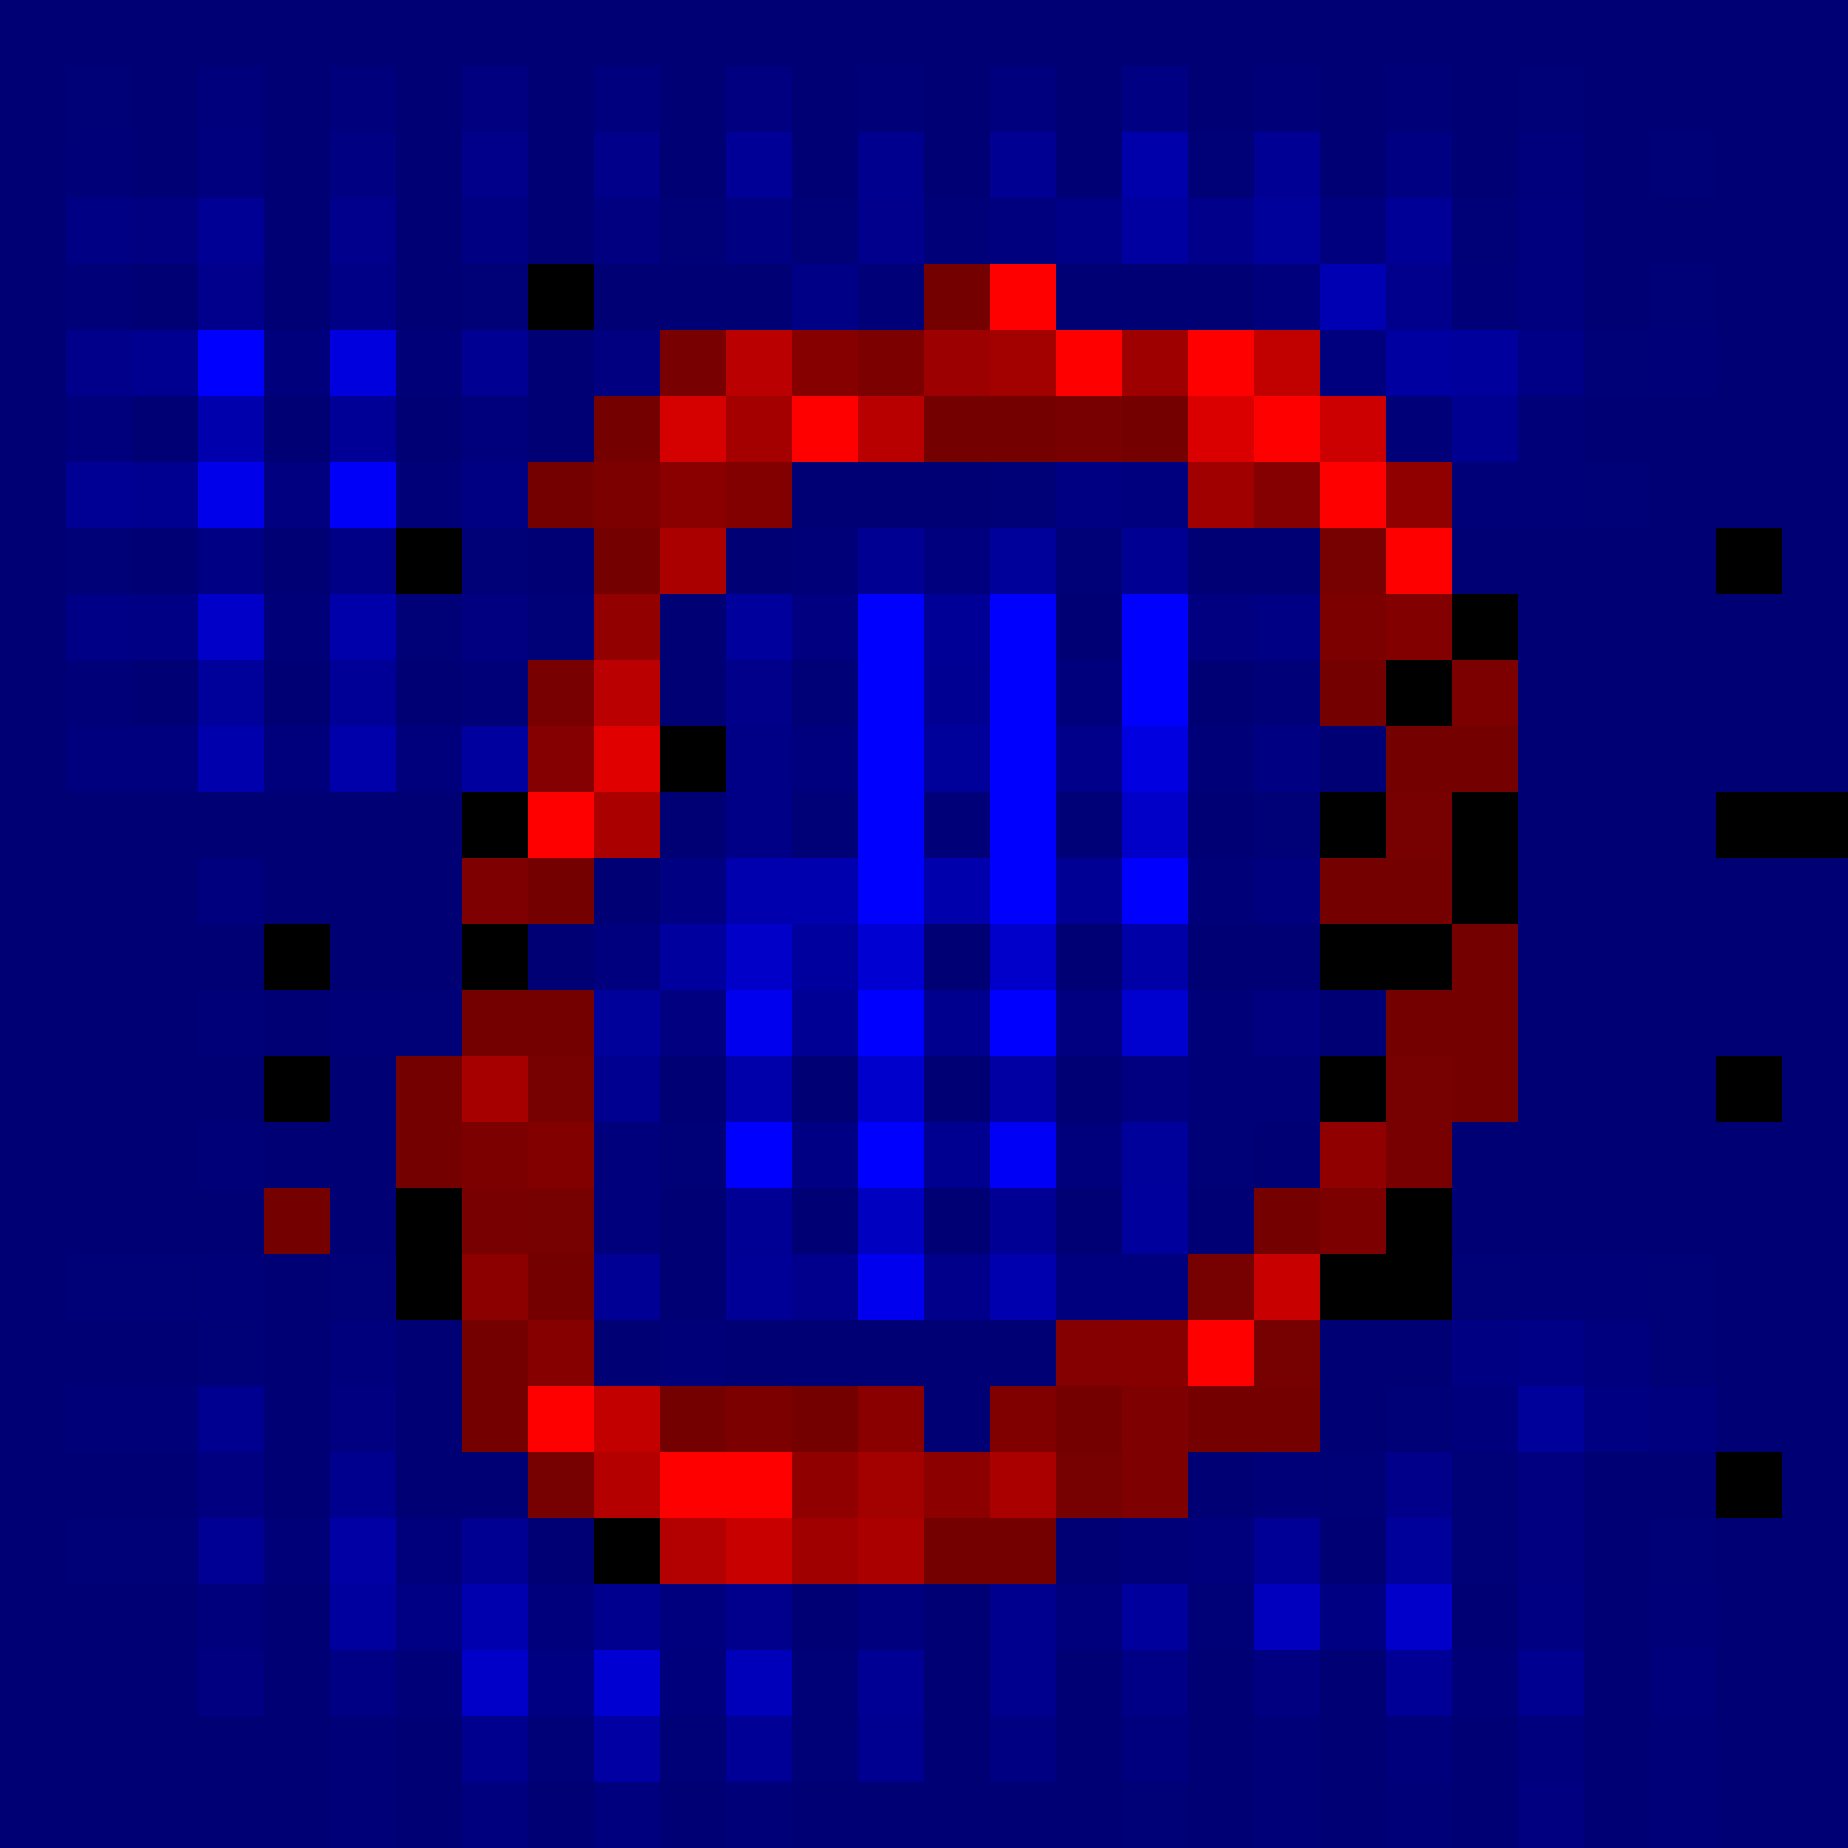
\includegraphics[width=\linewidth]{saliency/mnist_ic_saliency/saliency_threshold_wrt_0_bright.png}
        \scriptsize Gradient 0
    \end{minipage}%
    \begin{minipage}[b]{0.09\linewidth}\centering
        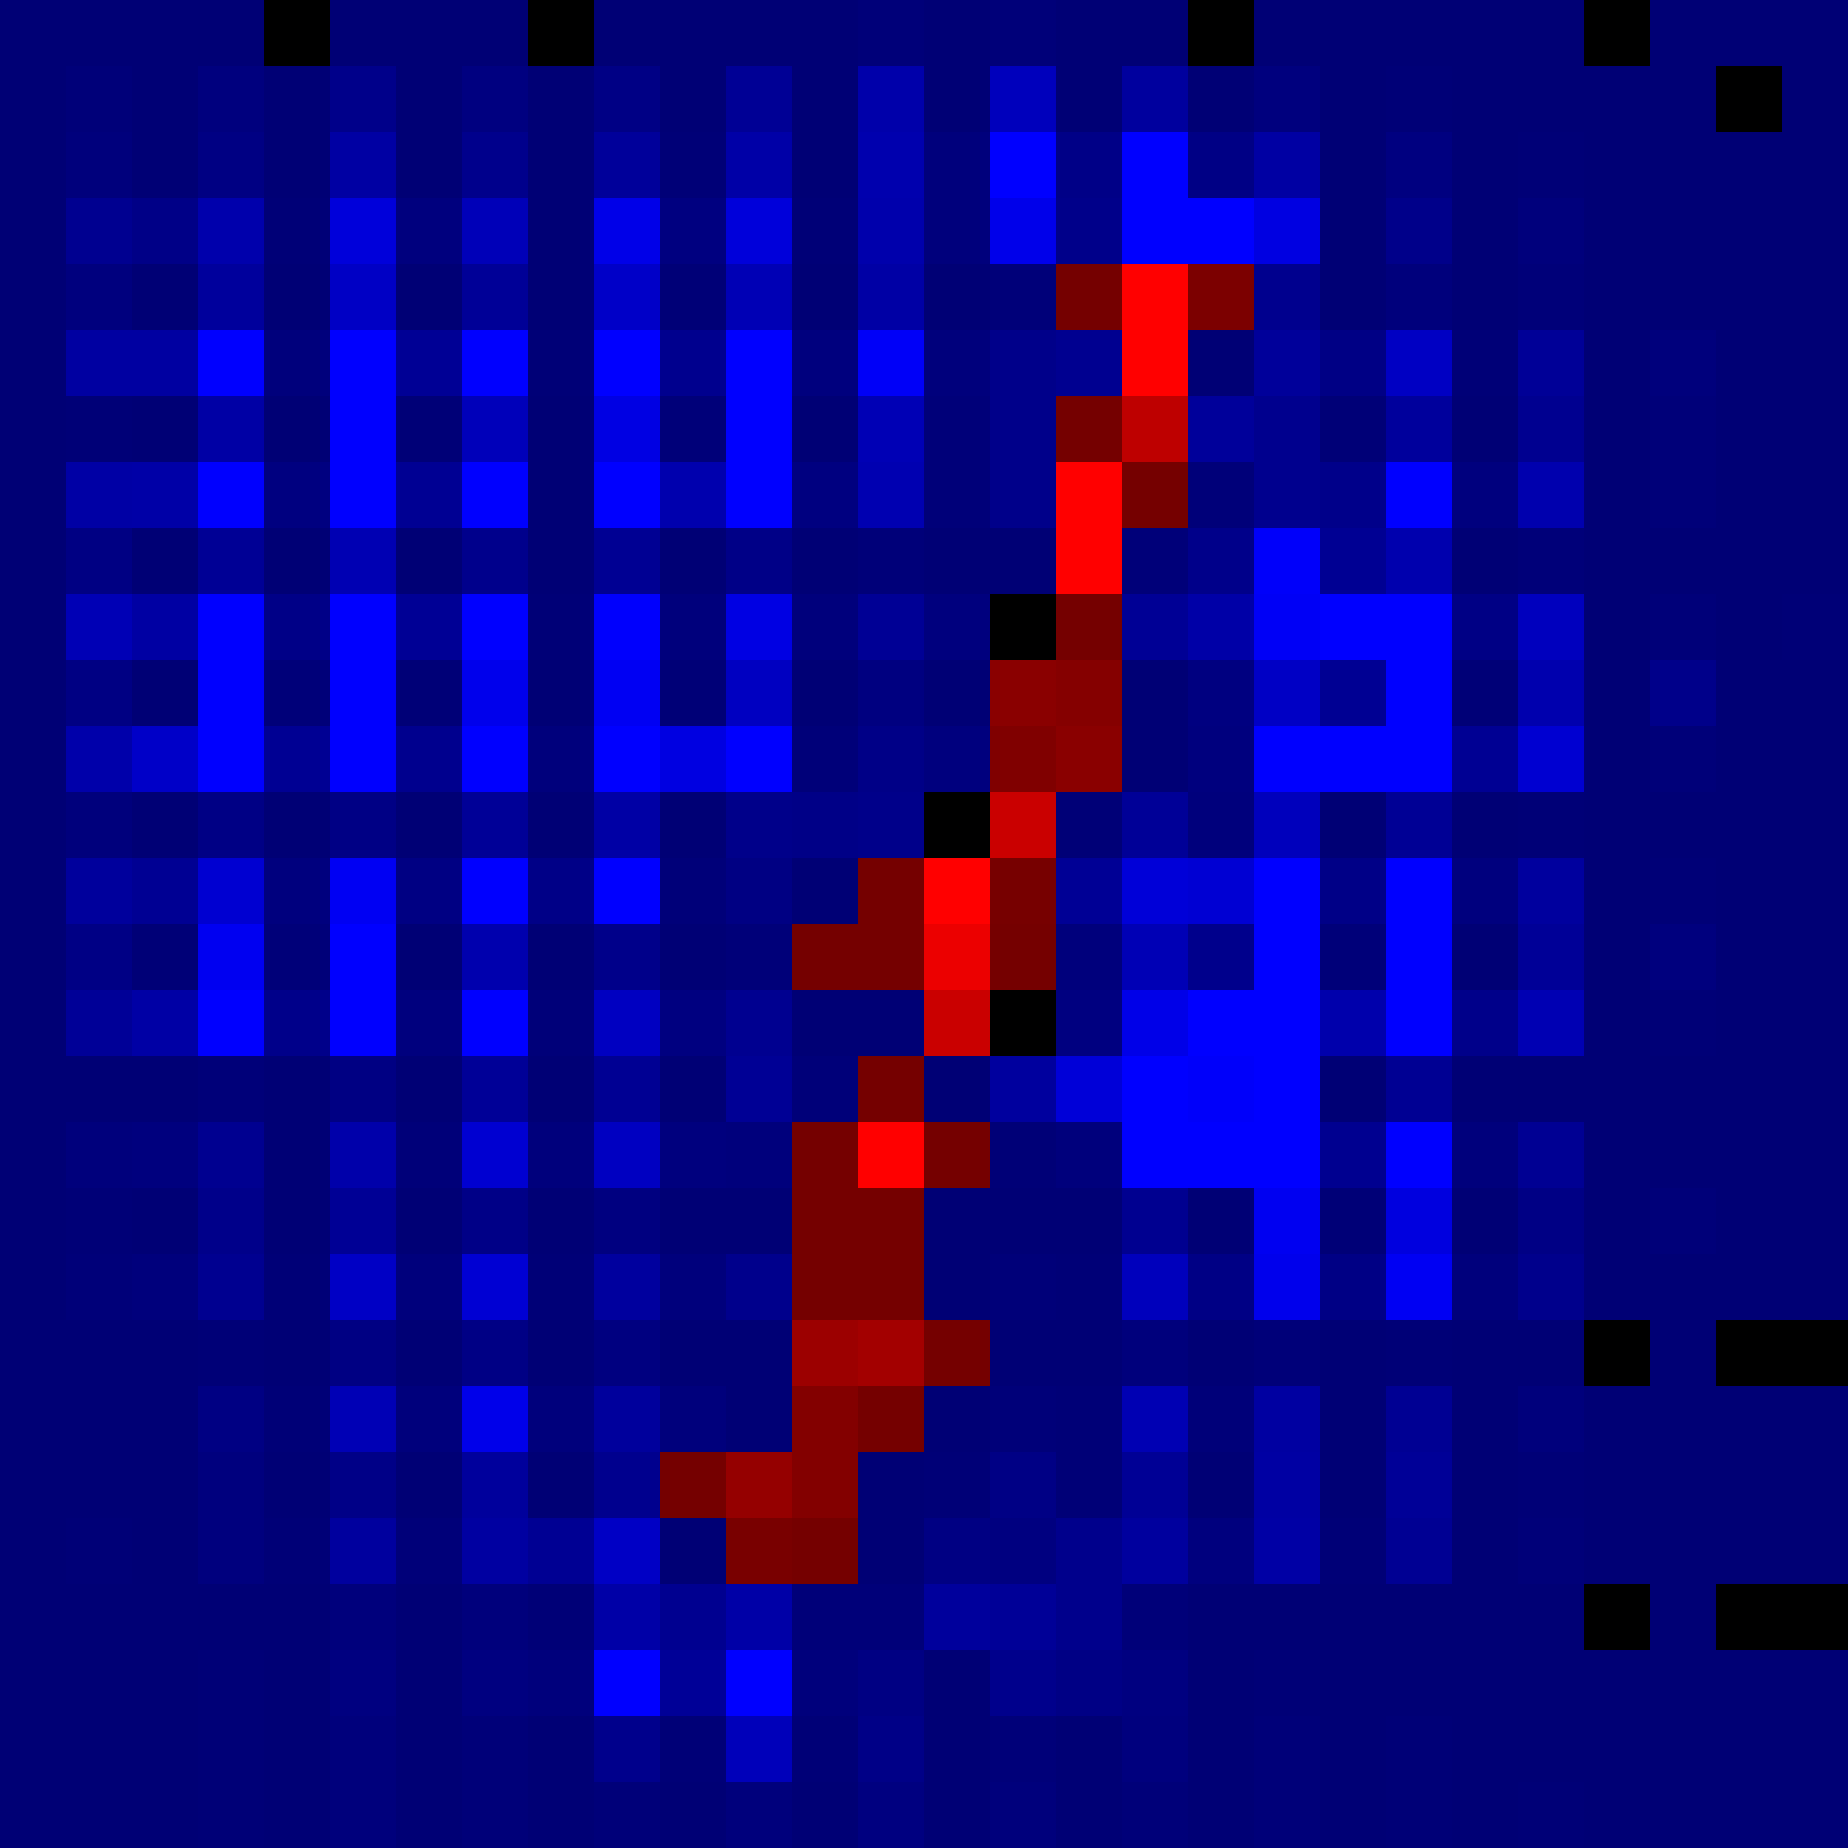
\includegraphics[width=\linewidth]{saliency/mnist_ic_saliency/saliency_threshold_wrt_1_bright.png}
        \scriptsize Gradient 1
    \end{minipage}%
    \begin{minipage}[b]{0.09\linewidth}\centering
        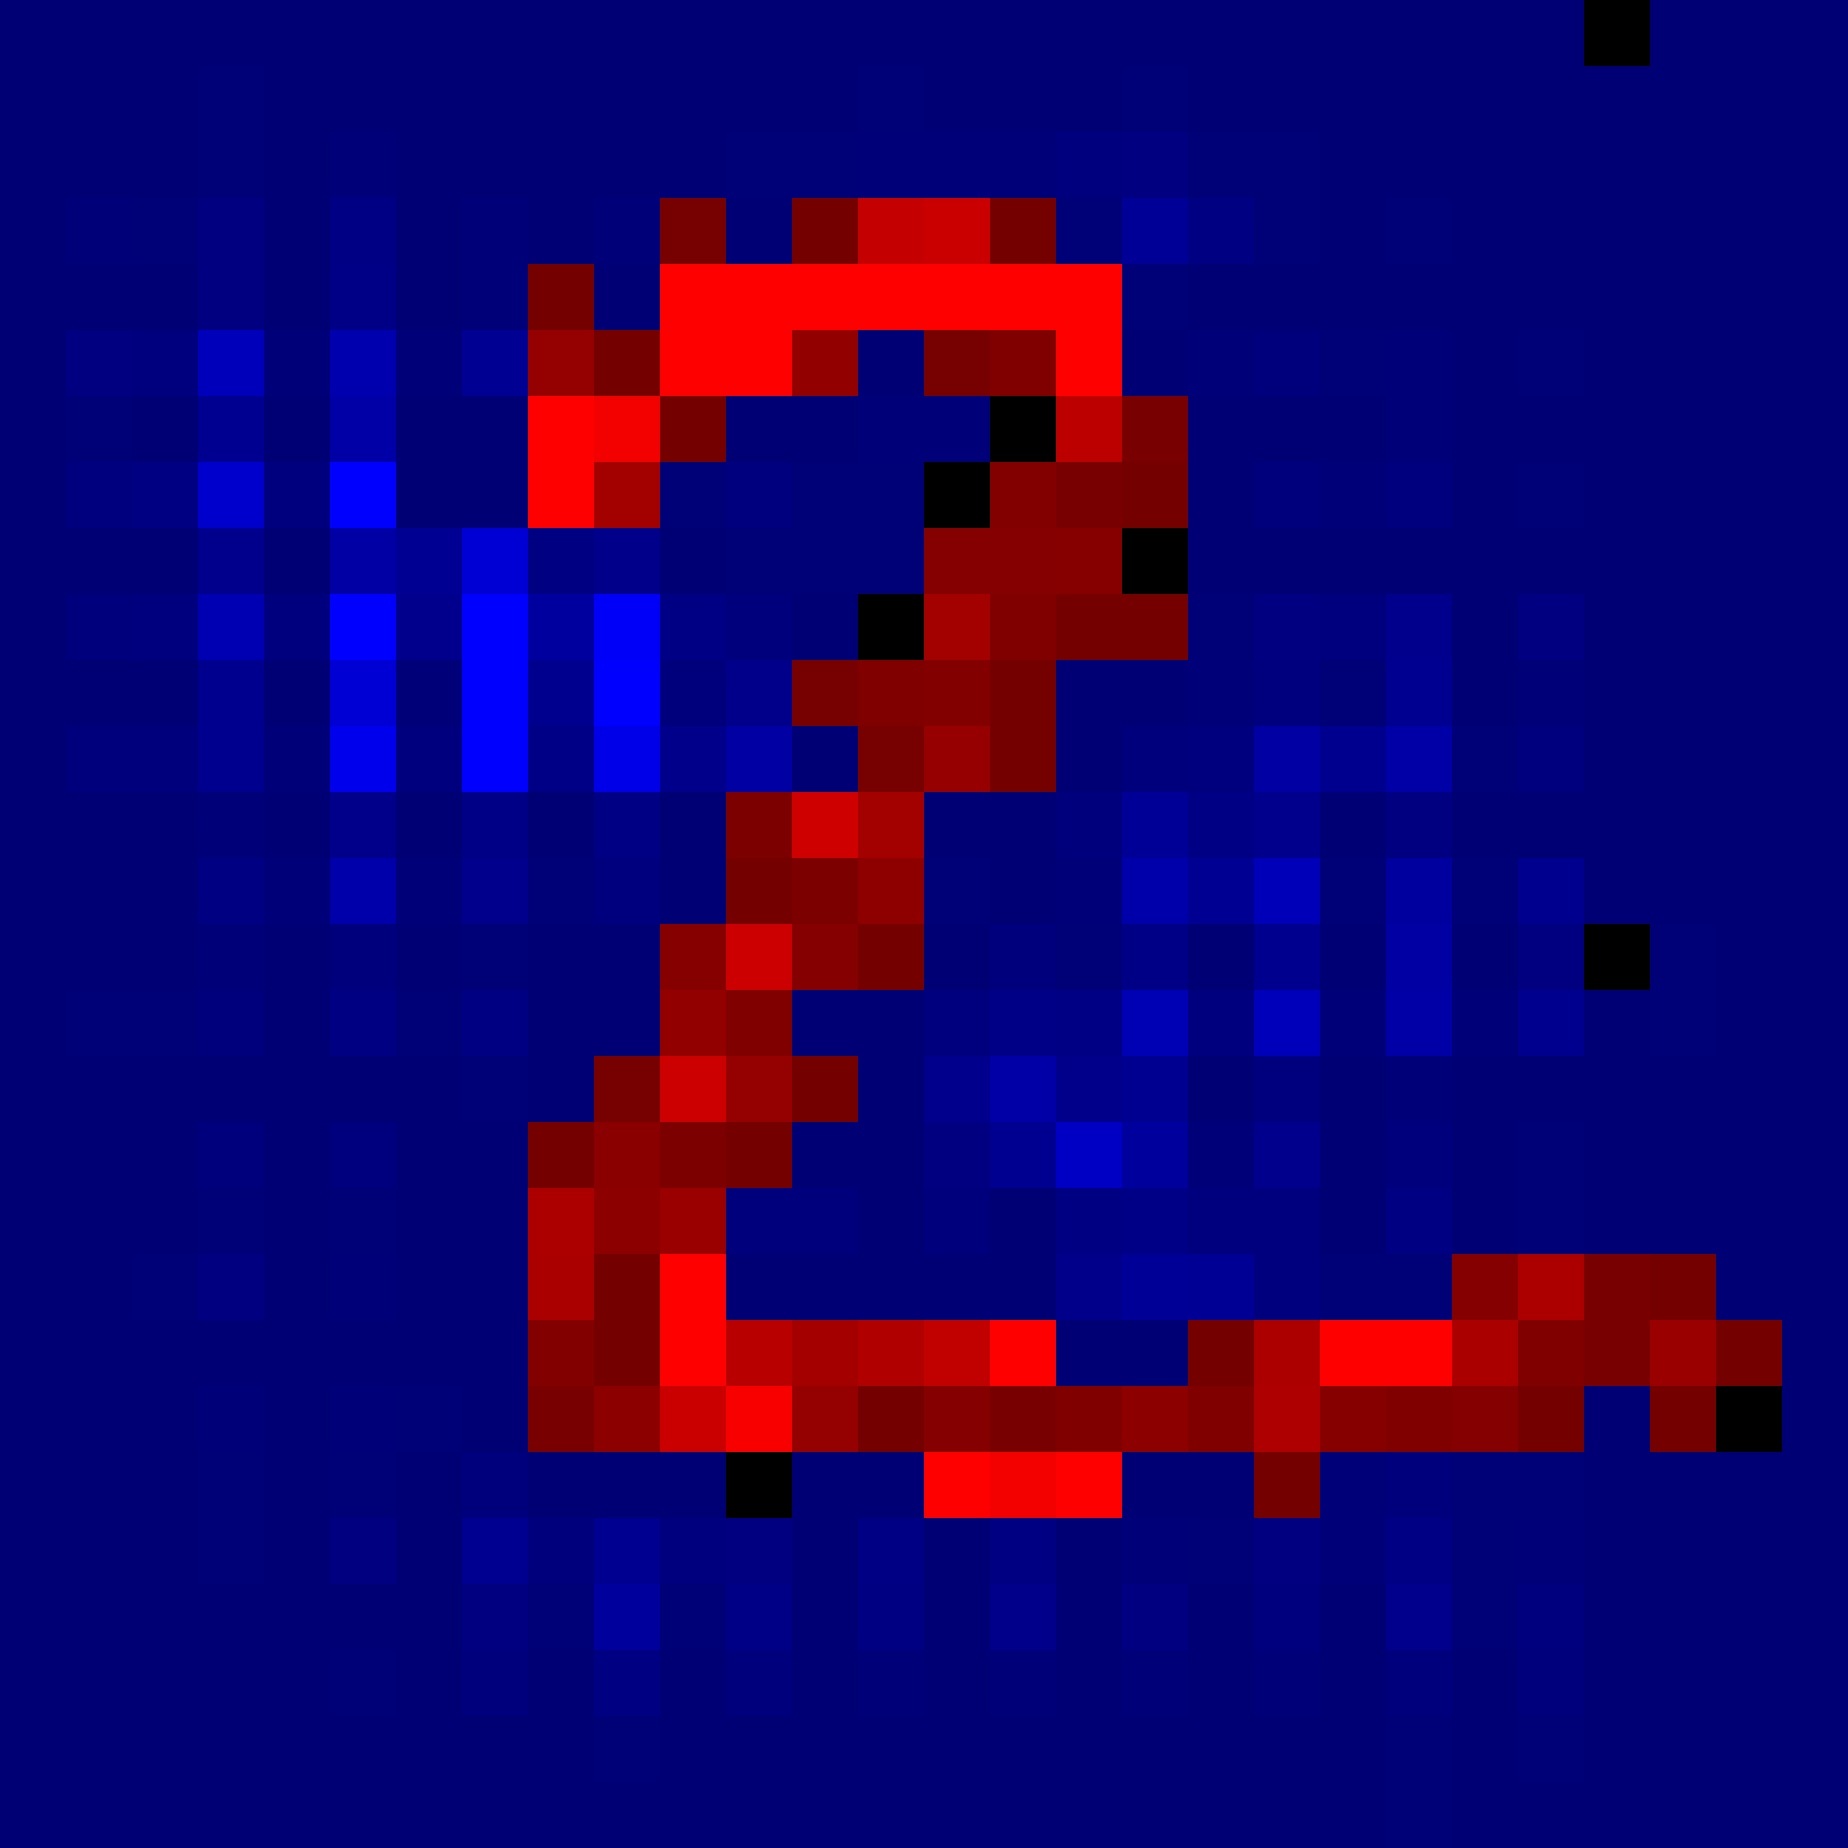
\includegraphics[width=\linewidth]{saliency/mnist_ic_saliency/saliency_threshold_wrt_2_bright.png}
        \scriptsize Gradient 2
    \end{minipage}%
    \begin{minipage}[b]{0.09\linewidth}\centering
        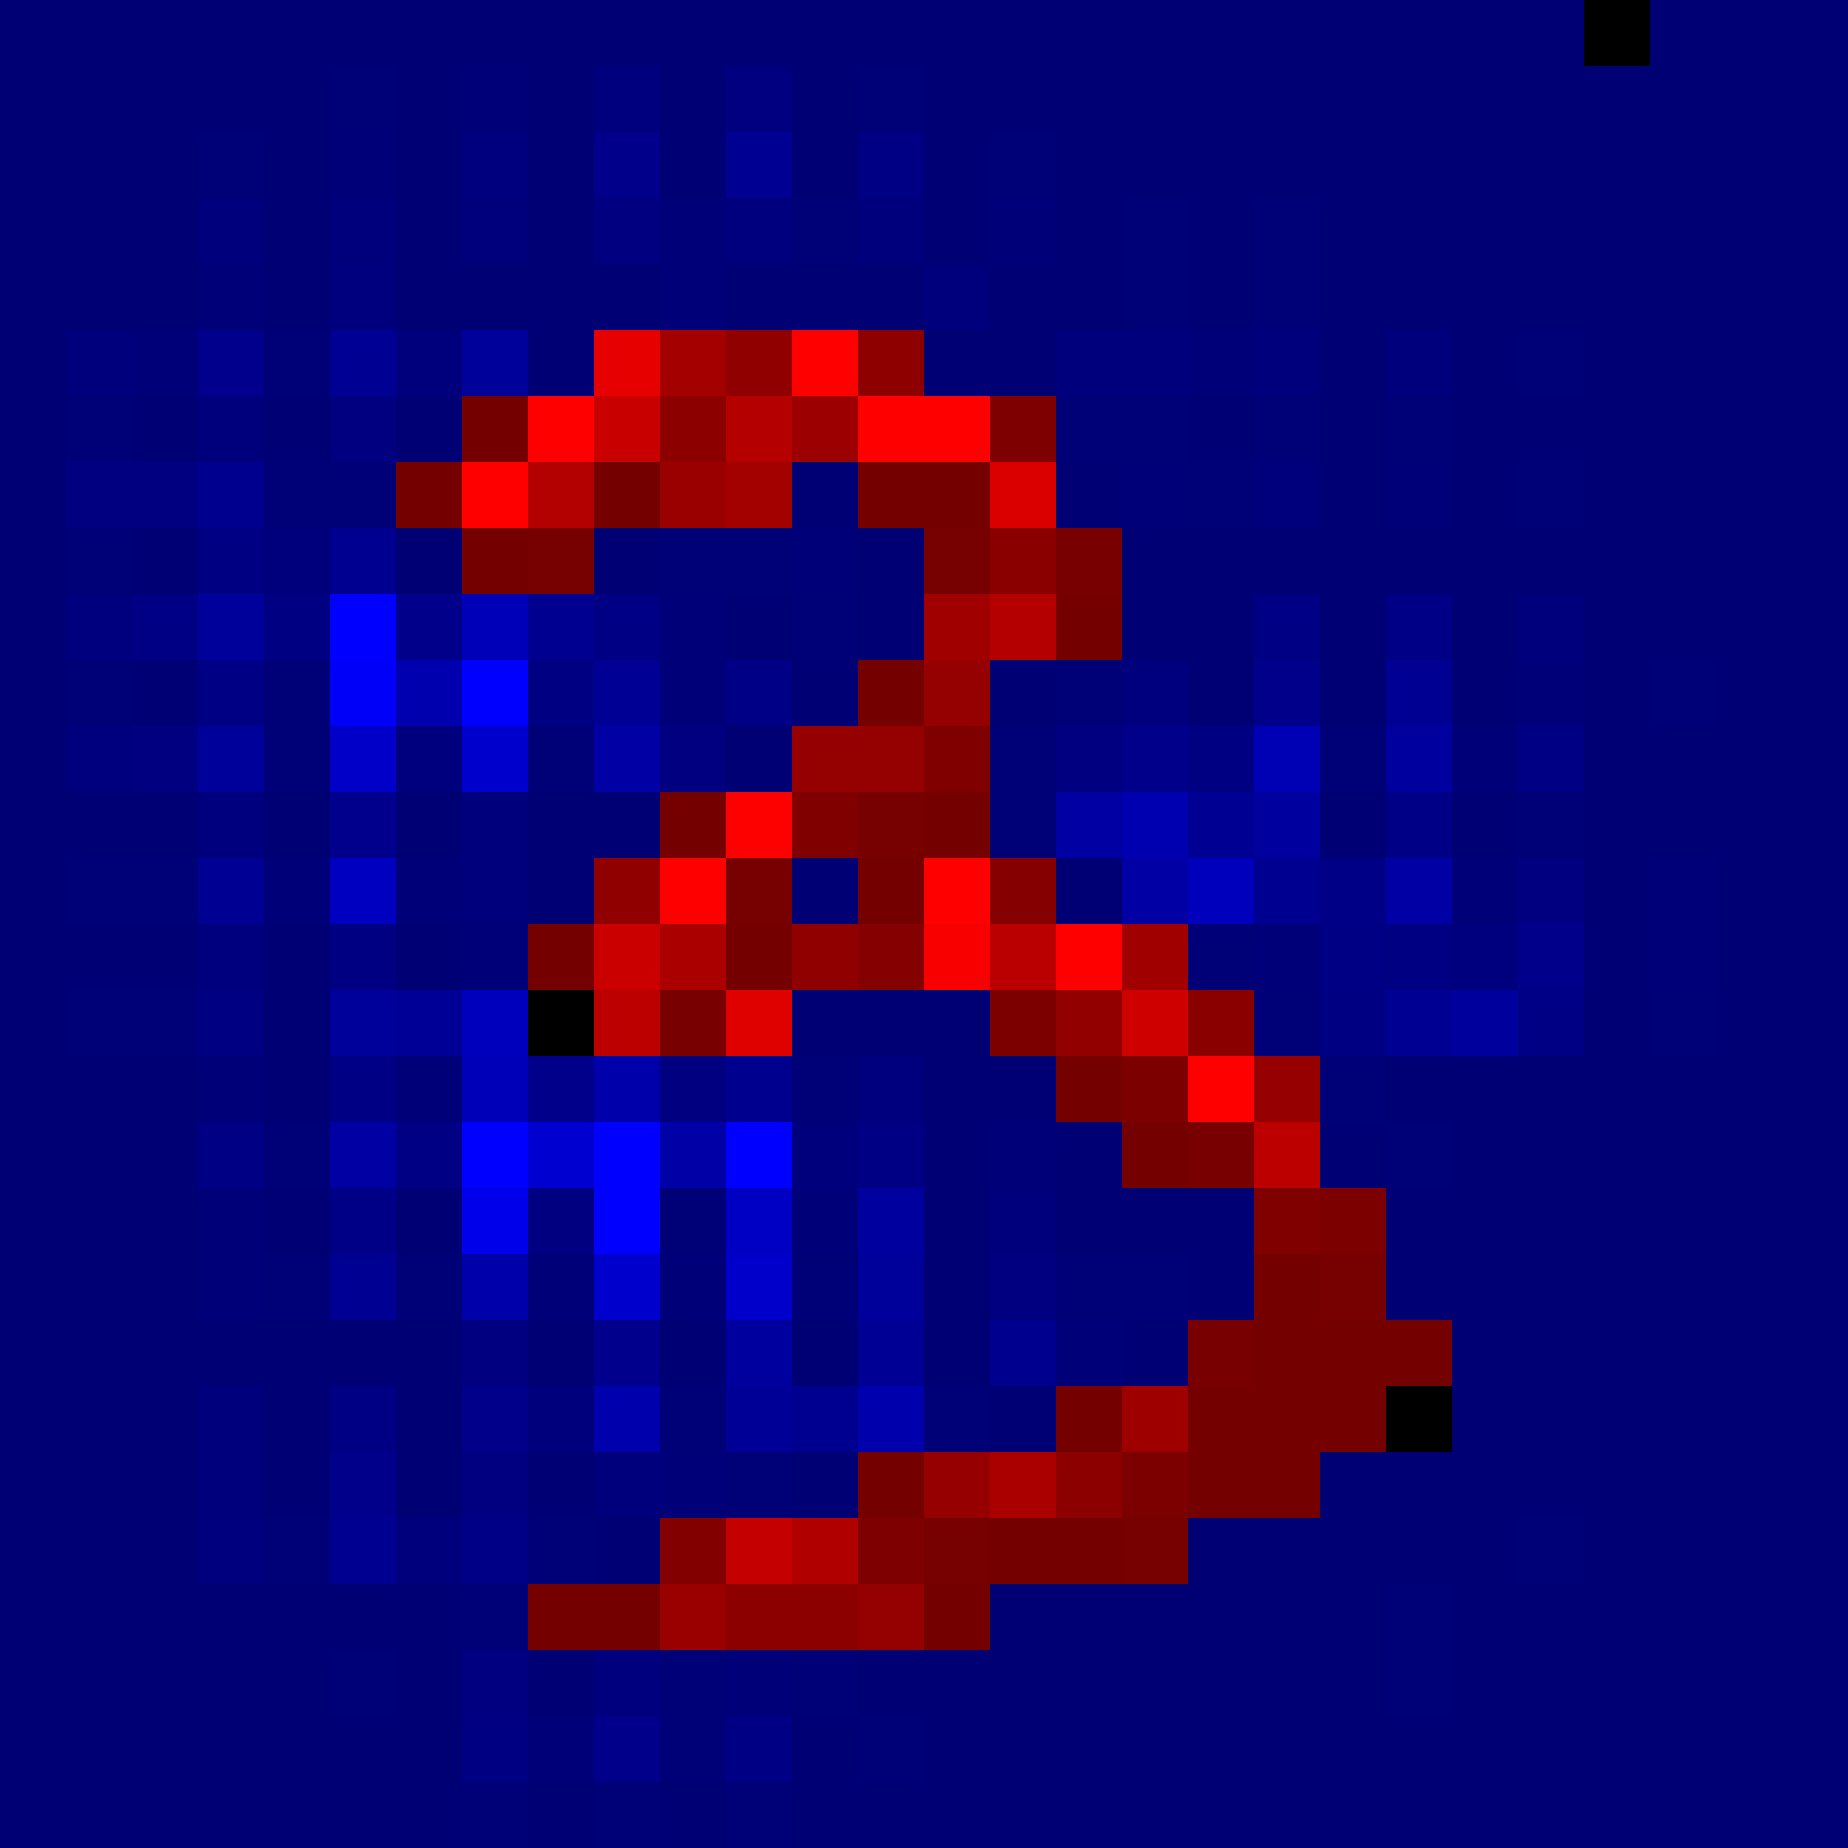
\includegraphics[width=\linewidth]{saliency/mnist_ic_saliency/saliency_threshold_wrt_3_bright.png}
        \scriptsize Gradient 3
    \end{minipage}%
    \begin{minipage}[b]{0.09\linewidth}\centering
        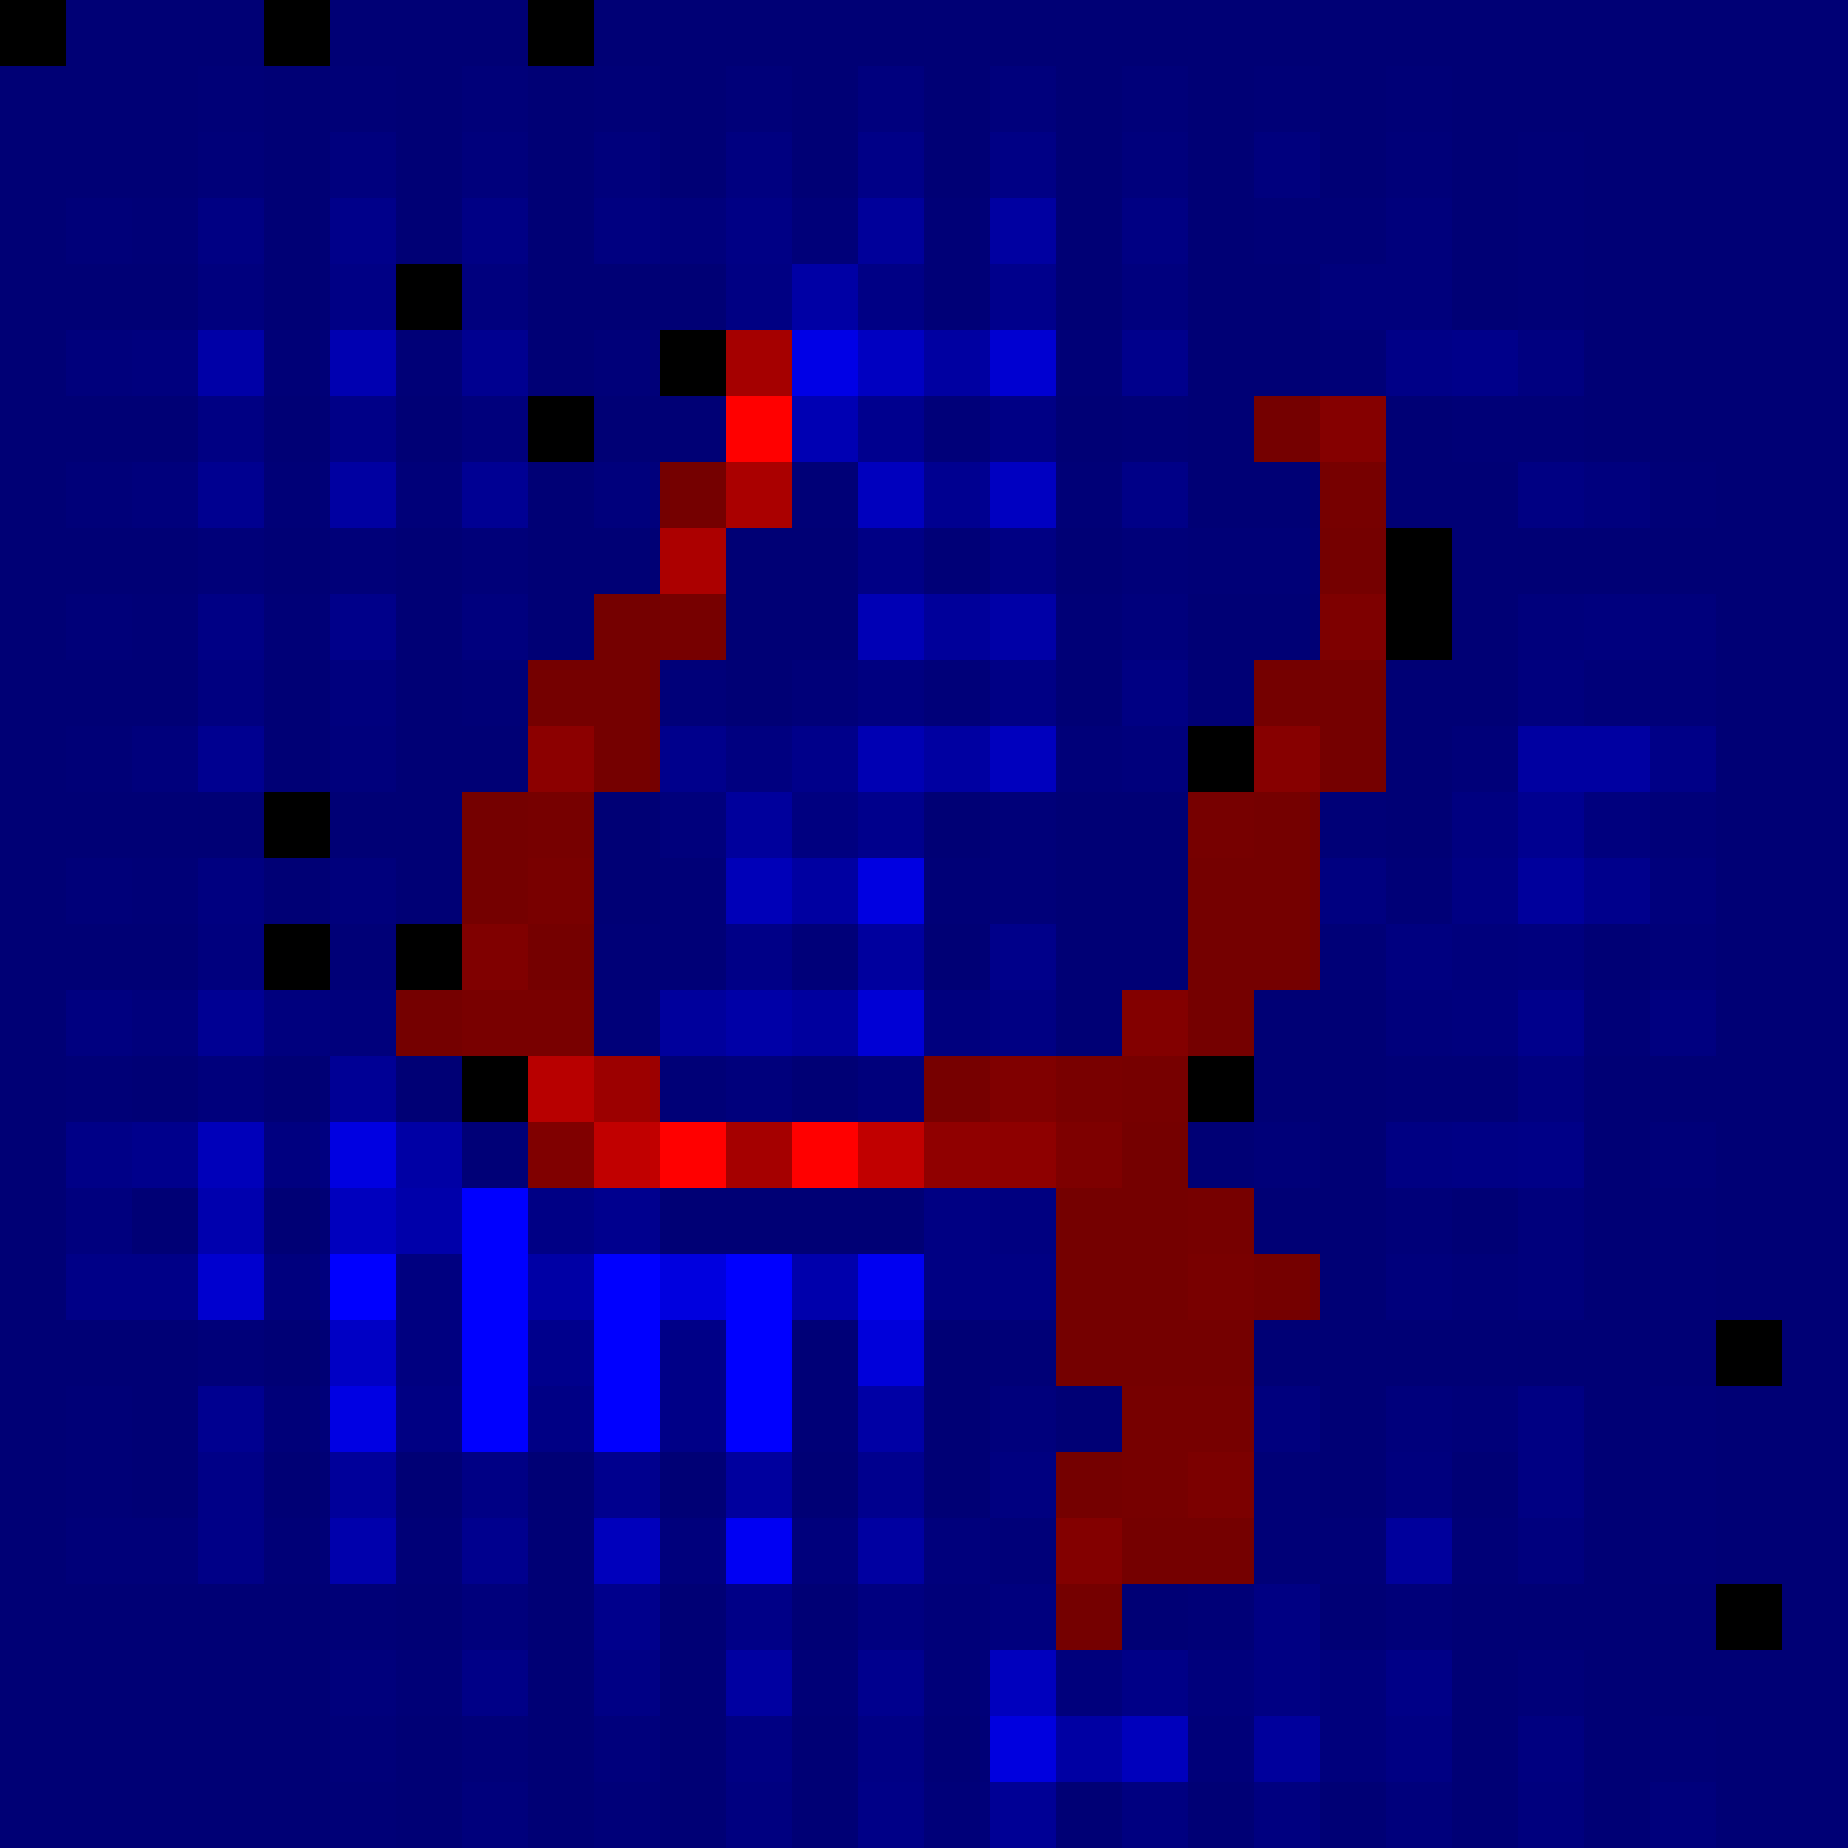
\includegraphics[width=\linewidth]{saliency/mnist_ic_saliency/saliency_threshold_wrt_4_bright.png}
        \scriptsize Gradient 4
    \end{minipage}%
    \begin{minipage}[b]{0.09\linewidth}\centering
        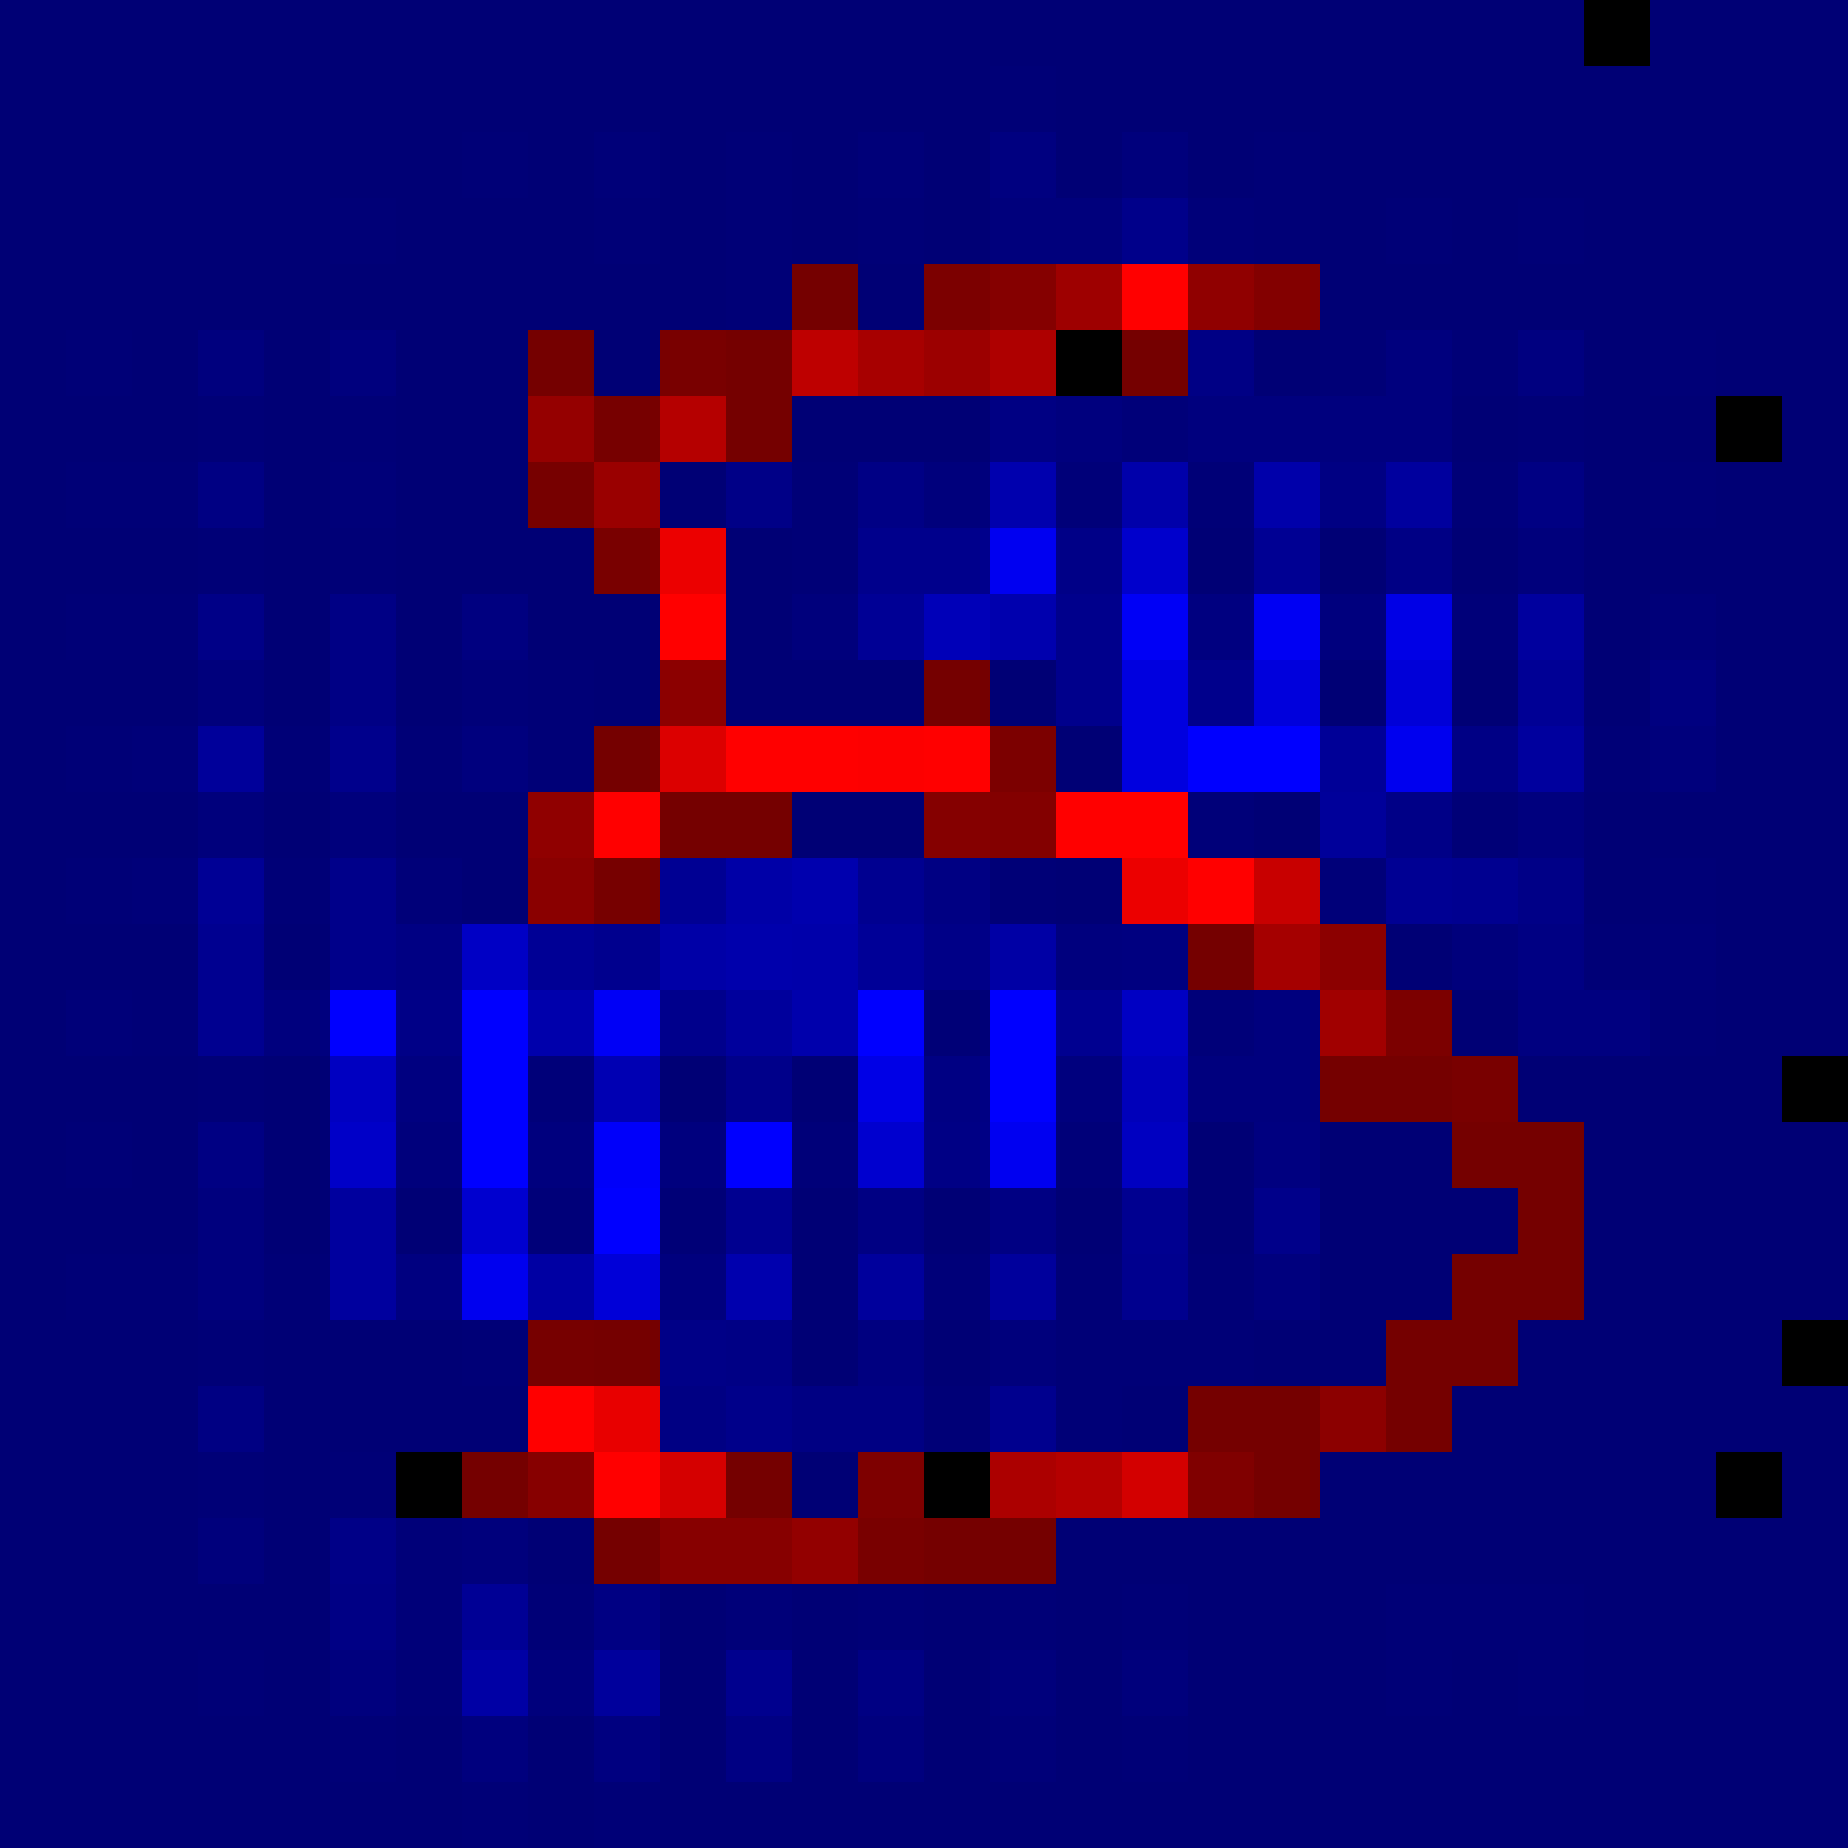
\includegraphics[width=\linewidth]{saliency/mnist_ic_saliency/saliency_threshold_wrt_5_bright.png}
        \scriptsize Gradient 5
    \end{minipage}%
    \begin{minipage}[b]{0.09\linewidth}\centering
        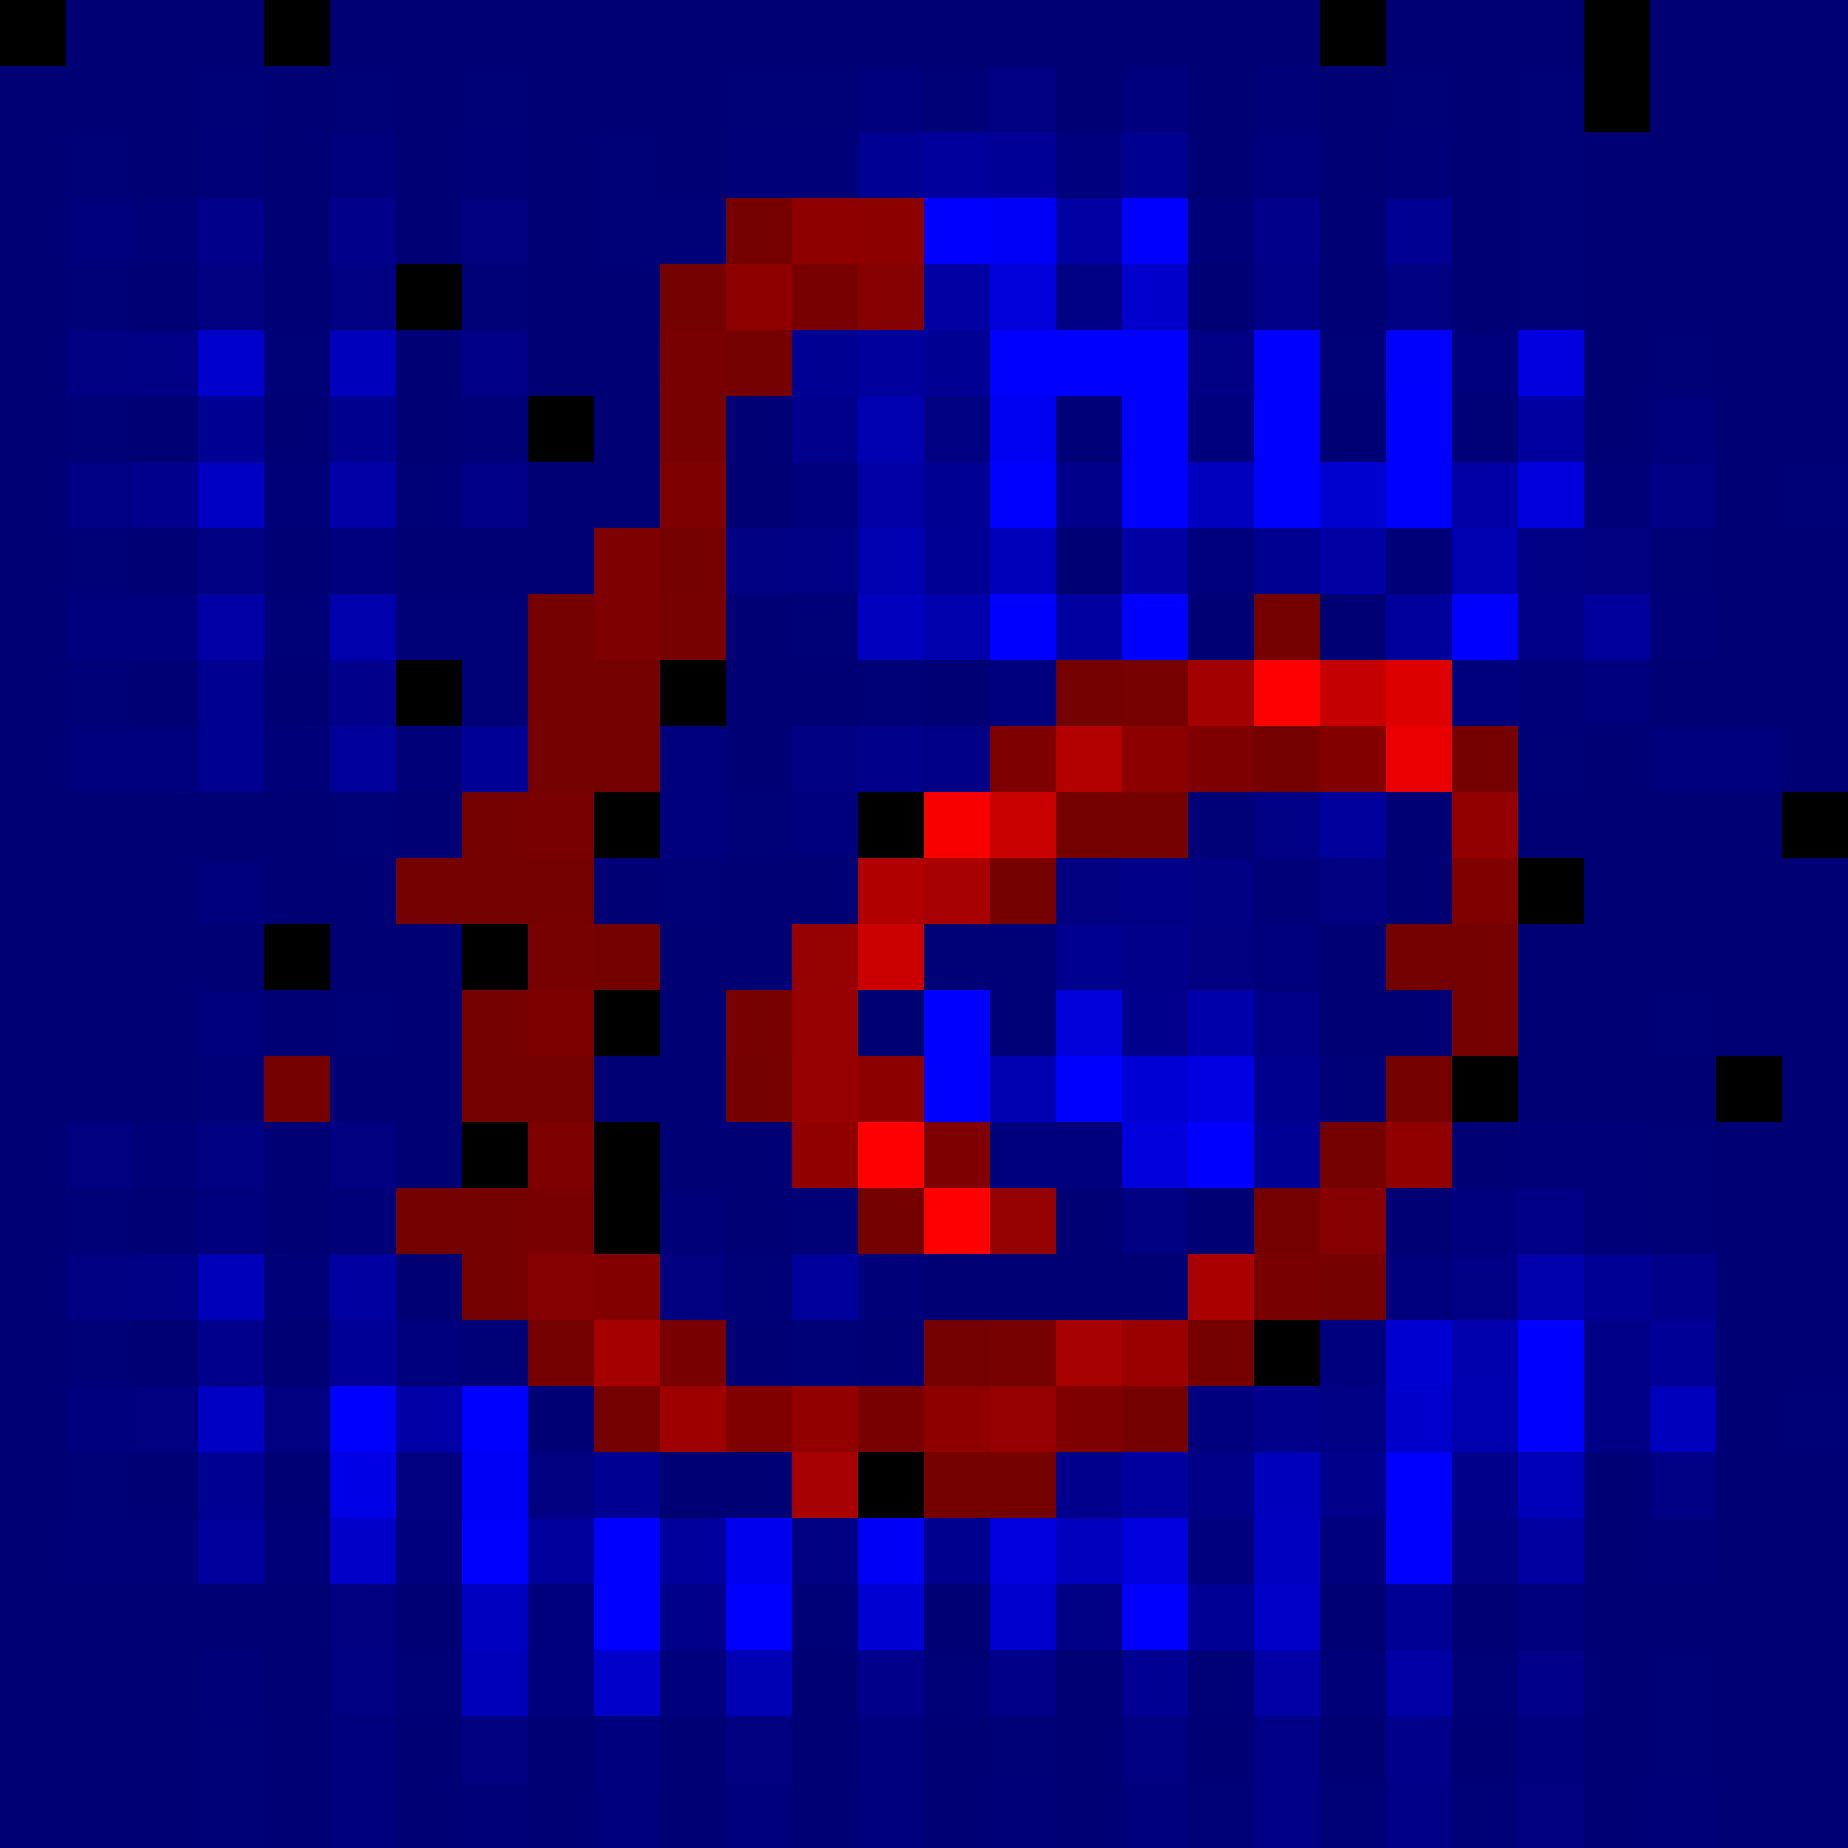
\includegraphics[width=\linewidth]{saliency/mnist_ic_saliency/saliency_threshold_wrt_6_bright.png}
        \scriptsize Gradient 6
    \end{minipage}%
    \begin{minipage}[b]{0.09\linewidth}\centering
        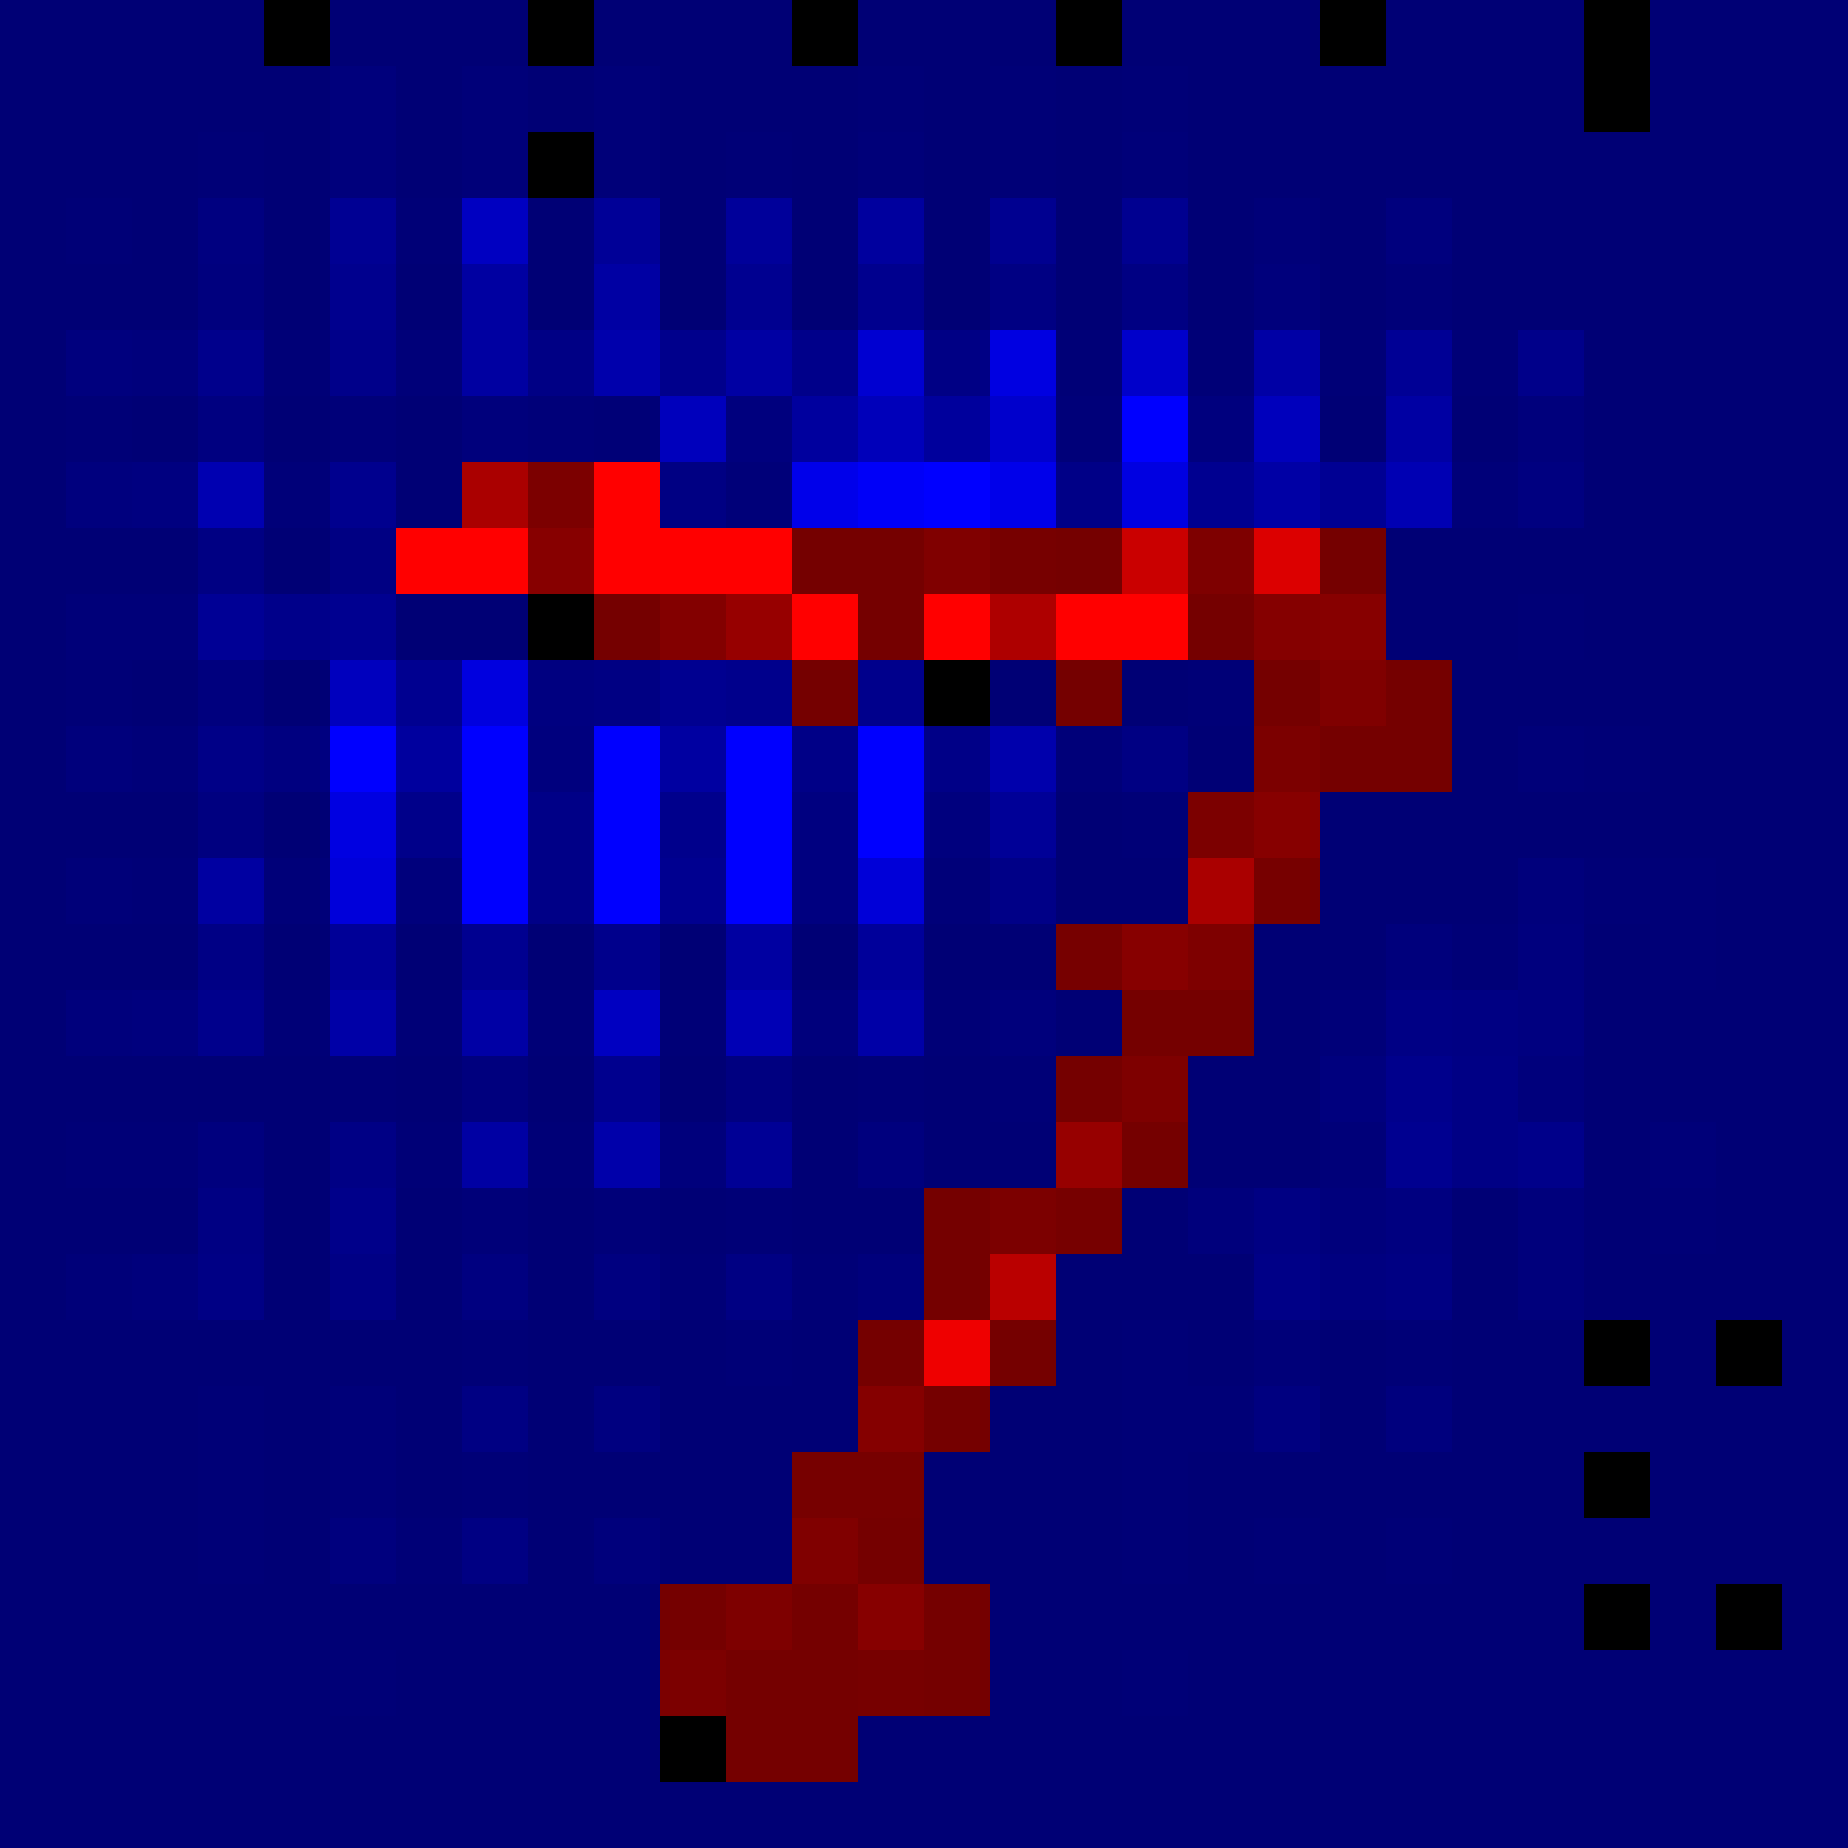
\includegraphics[width=\linewidth]{saliency/mnist_ic_saliency/saliency_threshold_wrt_7_bright.png}
        \scriptsize Gradient 7
    \end{minipage}%
    \begin{minipage}[b]{0.09\linewidth}\centering
        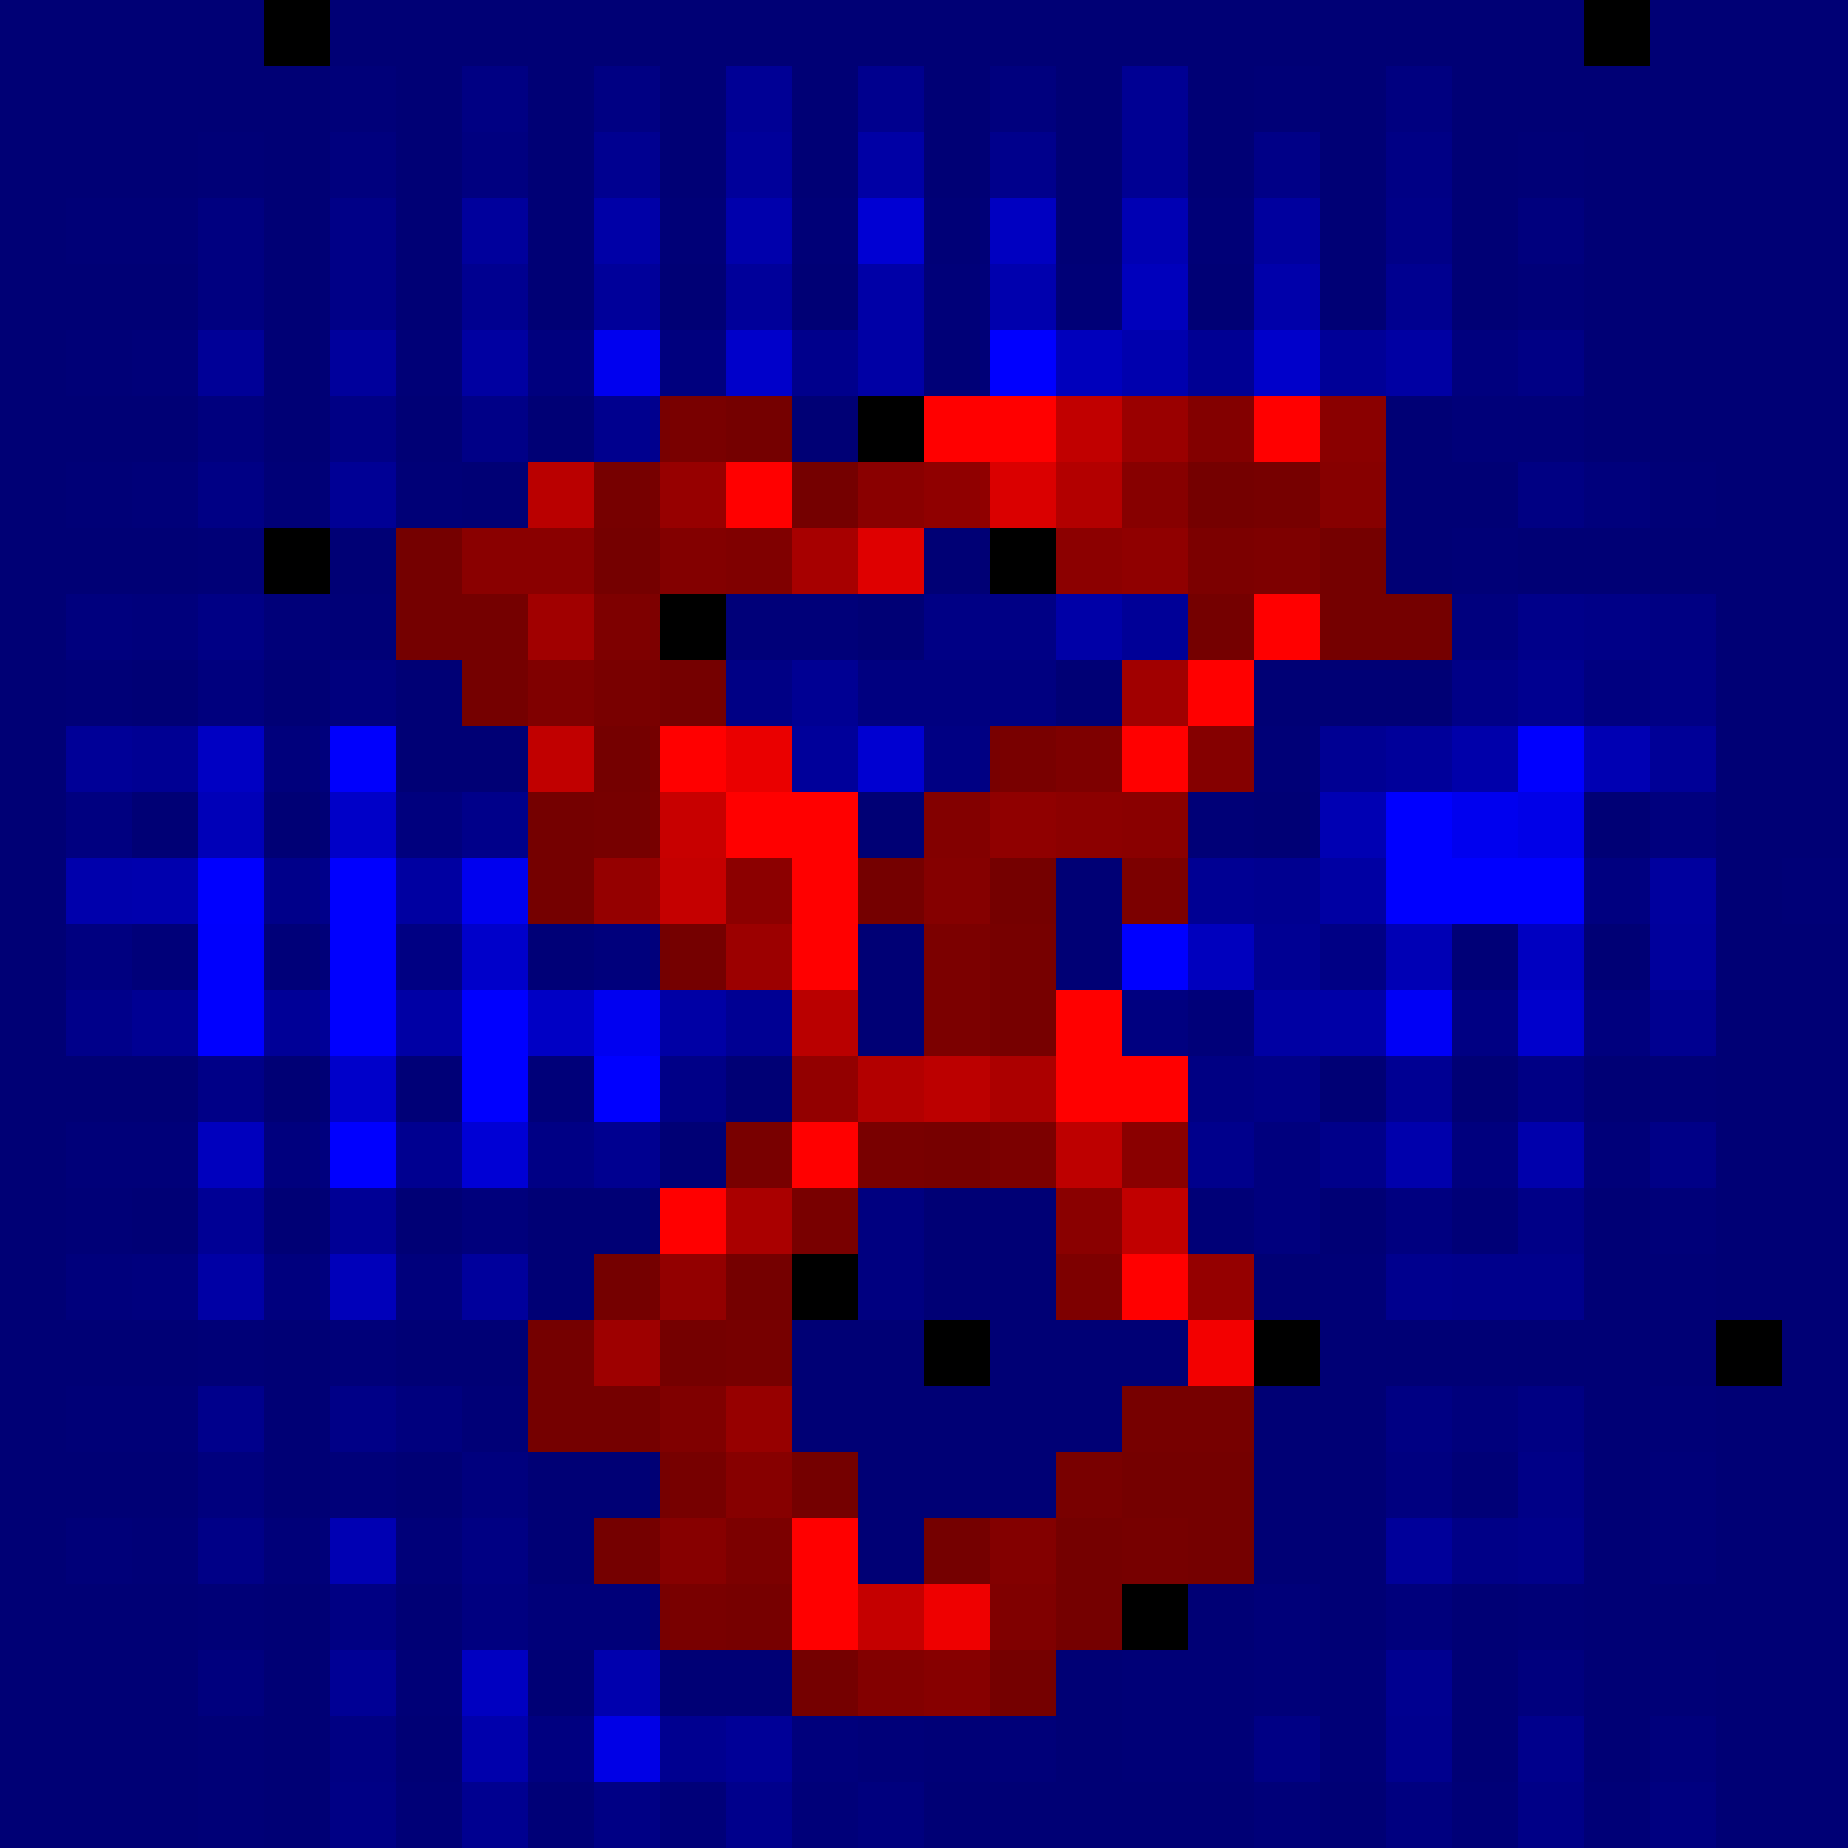
\includegraphics[width=\linewidth]{saliency/mnist_ic_saliency/saliency_threshold_wrt_8_bright.png}
        \scriptsize Gradient 8
    \end{minipage}%
    \begin{minipage}[b]{0.09\linewidth}\centering
        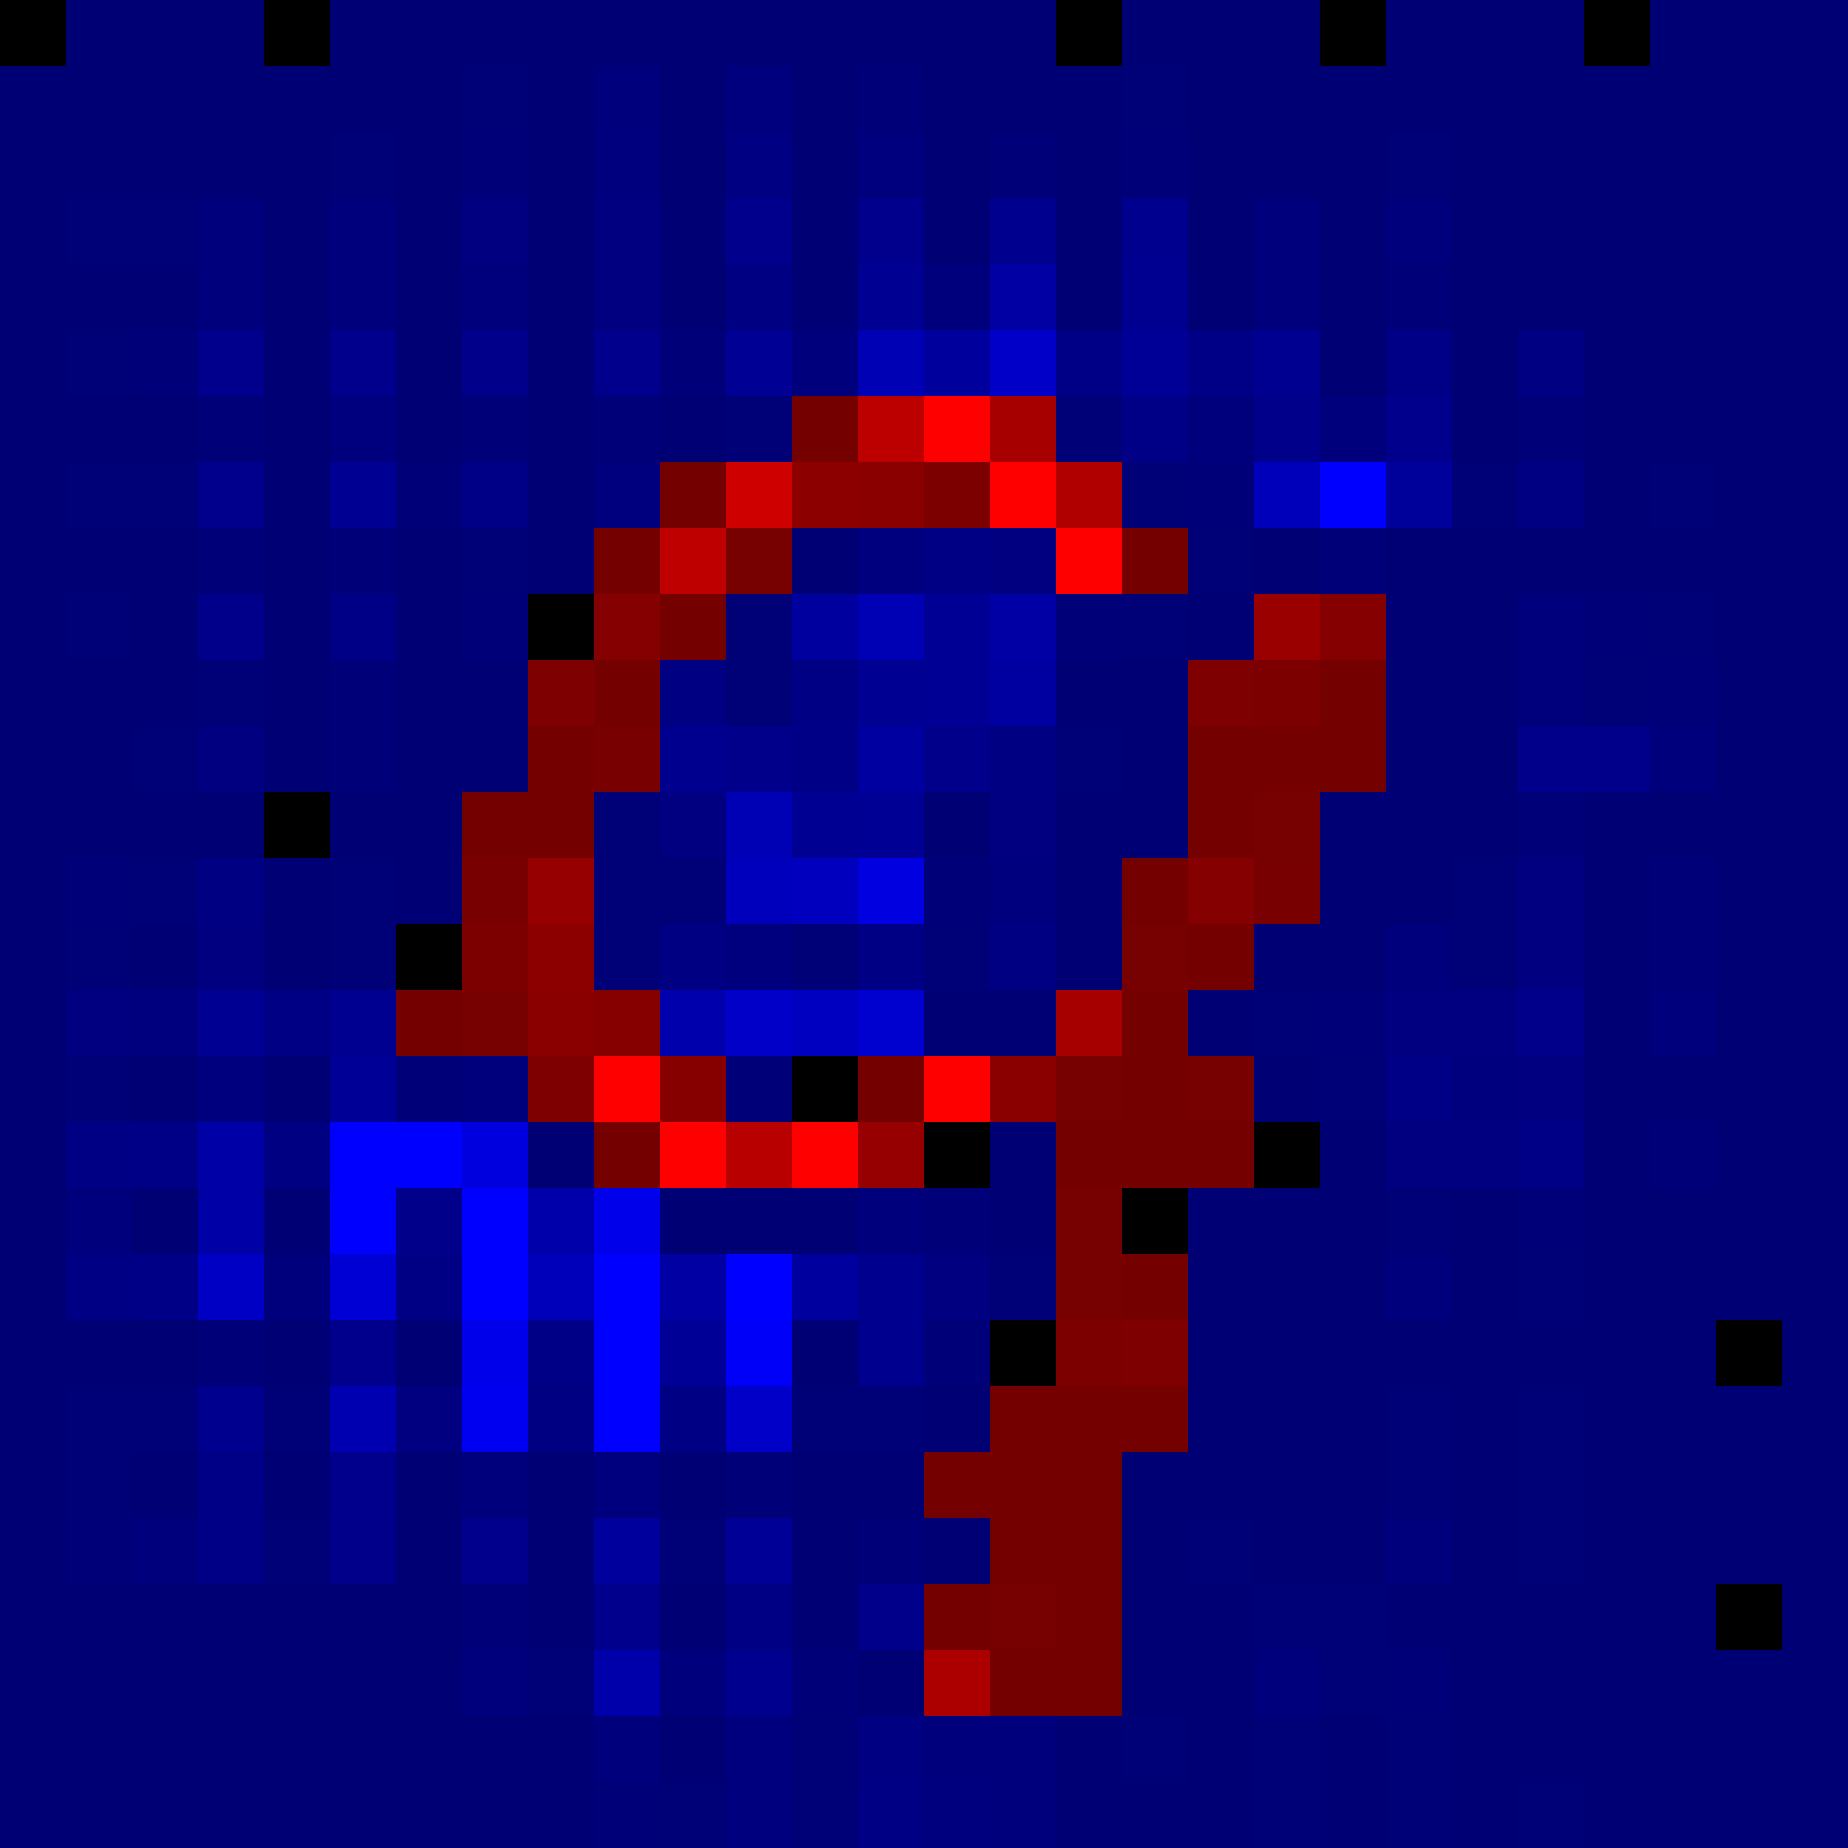
\includegraphics[width=\linewidth]{saliency/mnist_ic_saliency/saliency_threshold_wrt_9_bright.png}
        \scriptsize Gradient 9
    \end{minipage}%

    \par\vspace{0.25cm}
    \begin{minipage}[b]{0.09\linewidth}\centering
        
\includegraphics[width=\linewidth]{saliency/mnist_ic_saliency/original_0.png}
        \scriptsize Label 0
    \end{minipage}%
    \begin{minipage}[b]{0.09\linewidth}\centering
        
\includegraphics[width=\linewidth]{saliency/mnist_ic_saliency/original_1.png}
        \scriptsize Label 1
    \end{minipage}%
    \begin{minipage}[b]{0.09\linewidth}\centering
        
\includegraphics[width=\linewidth]{saliency/mnist_ic_saliency/original_2.png}
        \scriptsize Label 2
    \end{minipage}%
    \begin{minipage}[b]{0.09\linewidth}\centering
        
\includegraphics[width=\linewidth]{saliency/mnist_ic_saliency/original_3.png}
        \scriptsize Label 3
    \end{minipage}%
    \begin{minipage}[b]{0.09\linewidth}\centering
        
\includegraphics[width=\linewidth]{saliency/mnist_ic_saliency/original_4.png}
        \scriptsize Label 4
    \end{minipage}%
    \begin{minipage}[b]{0.09\linewidth}\centering
        
\includegraphics[width=\linewidth]{saliency/mnist_ic_saliency/original_5.png}
        \scriptsize Label 5
    \end{minipage}%
    \begin{minipage}[b]{0.09\linewidth}\centering
        
\includegraphics[width=\linewidth]{saliency/mnist_ic_saliency/original_6.png}
        \scriptsize Label 6
    \end{minipage}%
    \begin{minipage}[b]{0.09\linewidth}\centering
        
\includegraphics[width=\linewidth]{saliency/mnist_ic_saliency/original_7.png}
        \scriptsize Label 7
    \end{minipage}%
    \begin{minipage}[b]{0.09\linewidth}\centering
        
\includegraphics[width=\linewidth]{saliency/mnist_ic_saliency/original_8.png}
        \scriptsize Label 8
    \end{minipage}%
    \begin{minipage}[b]{0.09\linewidth}\centering
        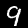
\includegraphics[width=\linewidth]{saliency/mnist_ic_saliency/original_9.png}
        \scriptsize Label 9
    \end{minipage}%

    }%
\caption[Input-gradient visualizations for ten MNIST digits]{Input-gradient visualizations of the \texttt{cnn\_maxout} IC model for ten MNIST digits, each with respect to its ground-truth label. Top: saliency maps; bottom: input images. As in the source figure, positive and negative gradient values above threshold 0.2 are colored red and blue, with ranking colorized using exponential decay.}
    \label{fig:mnist_ic_saliency}
\end{figure}


\paragraph{Accuracy trade-offs.}\label{subsec:dcinn_accuracy}

Table~\ref{tab:cdinn_acc} reports the median test accuracy of all eight variants over ten seeds. For the \ac{mlp}, every difference-of-two variant exceeds the unrestricted baseline's median accuracy of $98.39\%$, reaching $98.58\%$ for DICIN. For the \ac{cnn}, IC achieves $99.16\%$, close to the unrestricted model's $99.19\%$; difference-of-two variants reach $97.94$--$98.28\%$.

\section{Game-Based Case Study}\label{sec:results_vit}\label{sec:saliency_results}\label{ptnb:sec:experiments}\label{ptnb:sec:case-study}



\paragraph{Protocol.}
Methods are evaluated under a two-stage protocol that treats baselines and our games alike. Stage~1 runs a validation grid search for every tunable method, including DAVE (Table~\ref{ptnb:tab:main-search-grid}; \nValGrid{} configurations in total). Stage~2 independently selects the localization and faithfulness rank-sum configurations and evaluates both once on the test split. Confidence intervals and Holm-corrected paired comparisons follow Section~\ref{ptnb:app:stats}. The \ac{rg}/\ac{rg}+Eq anchors additionally represent $\alpha\beta$-\ac{lrp} exactly (Theorem~\ref{ptnb:thm:lrp-recovery}). Table~\ref{ptnb:tab:eval-vit} reports the paper's selected localization configurations and anchors, with their original testing family. Table~\ref{ptnb:tab:test-ci-vit} in Appendix~\ref{ptnb:app:test-ci} gives both selections, further baselines and confidence intervals. Reporting faithfulness-selected rows separately preserves the distinction between mask agreement and faithfulness.

% Selected ViT-B/16 results; the full localization/faithfulness comparison is
% reported in Appendix Table~\ref{ptnb:tab:test-ci-vit}.
\begin{table}[tbp]
    \centering
    \caption[Selected ViT-B/16 attribution results]{ViT-B/16 on the ImageNet-S test split (565 images): localization-selected configurations and the theorem-fixed RG/RG+Eq anchors. Cells report means with 95\% bootstrap confidence intervals; MaxS and AvgS use the fixed 200-image subset. Bold/dark shading marks the best displayed value per metric; $^{\approx}$/light shading marks no detected difference from it under Holm-corrected paired tests over the selected main-table rows. Runtime is seconds per image. Full localization- and faithfulness-selected results with additional baselines appear in Table~\ref{ptnb:tab:test-ci-vit} in Appendix~\ref{ptnb:app:test-ci}.}
    \label{ptnb:tab:eval-vit}\label{tab:eval-vit}
    \TableContent{
        \fontsize{8.5pt}{9.2pt}\selectfont
        \setlength{\tabcolsep}{1pt}
        \renewcommand{\arraystretch}{0.9}
        \appfitgen{tables/ptnb_v2/generated/main_vit_tabular}
    }%
\end{table}

\begin{figure}[htbp]
\QualitativeImageContent{
    \centering
    \setlength{\tabcolsep}{0.6pt}
    \renewcommand{\arraystretch}{0.3}
    \resizebox{\textwidth}{!}{
    \begin{tabular}{@{}r *{11}{c}@{}}
        & {\scriptsize Orig.}
        & {\scriptsize Mask}
        & {\scriptsize RG (loc)}
        & {\scriptsize RG+Eq (loc)}
        & {\scriptsize Grad}
        & {\scriptsize SmGrad}
        & {\scriptsize IntGrad}
        & {\scriptsize DAVE}
        & {\scriptsize LRP-$\gamma$}
        & {\scriptsize AttnLRP}
        & {\scriptsize TIBAV} \\[2pt]
        \rotatebox{90}{\scriptsize\hspace{2pt}Red fox (snow)}
        & 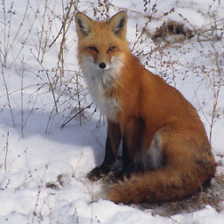
\includegraphics[width=0.085\textwidth]{figures/ptnb_v2/qualitative/butterfly/red_fox_snow/original.png}
        & 
\includegraphics[width=0.085\textwidth]{figures/ptnb_v2/qualitative/butterfly/red_fox_snow/mask.png}
        & 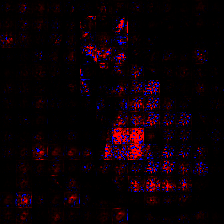
\includegraphics[width=0.085\textwidth]{figures/ptnb_v2/qualitative/butterfly/red_fox_snow/rg_loc.png}
        & 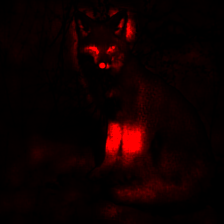
\includegraphics[width=0.085\textwidth]{figures/ptnb_v2/qualitative/butterfly/red_fox_snow/rgeq_loc.png}
        & 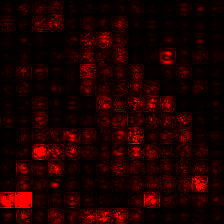
\includegraphics[width=0.085\textwidth]{figures/ptnb_v2/qualitative/butterfly/red_fox_snow/gradient.png}
        & 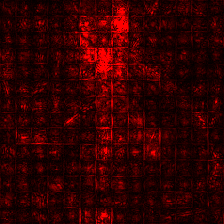
\includegraphics[width=0.085\textwidth]{figures/ptnb_v2/qualitative/butterfly/red_fox_snow/smooth_grad.png}
        & 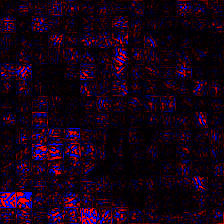
\includegraphics[width=0.085\textwidth]{figures/ptnb_v2/qualitative/butterfly/red_fox_snow/integrated_gradients.png}
        & 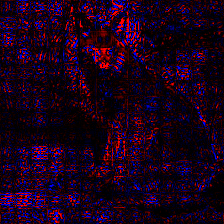
\includegraphics[width=0.085\textwidth]{figures/ptnb_v2/qualitative/butterfly/red_fox_snow/dave.png}
        & 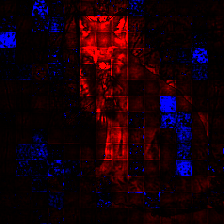
\includegraphics[width=0.085\textwidth]{figures/ptnb_v2/qualitative/butterfly/red_fox_snow/lrp_gamma.png}
        & 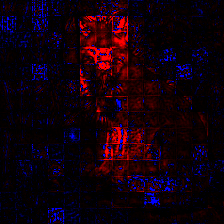
\includegraphics[width=0.085\textwidth]{figures/ptnb_v2/qualitative/butterfly/red_fox_snow/attn_lrp.png}
        & 
\includegraphics[width=0.085\textwidth]{figures/ptnb_v2/qualitative/butterfly/red_fox_snow/tibav.png} \\[1pt]
        \rotatebox{90}{\scriptsize\hspace{6pt}Red fox}
        & 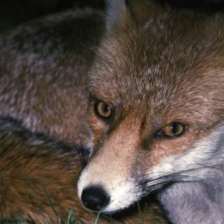
\includegraphics[width=0.085\textwidth]{figures/ptnb_v2/qualitative/butterfly/red_fox/original.png}
        & 
\includegraphics[width=0.085\textwidth]{figures/ptnb_v2/qualitative/butterfly/red_fox/mask.png}
        & 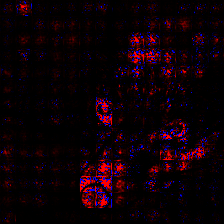
\includegraphics[width=0.085\textwidth]{figures/ptnb_v2/qualitative/butterfly/red_fox/rg_loc.png}
        & 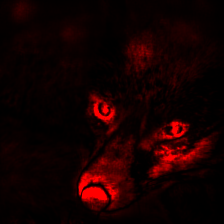
\includegraphics[width=0.085\textwidth]{figures/ptnb_v2/qualitative/butterfly/red_fox/rgeq_loc.png}
        & 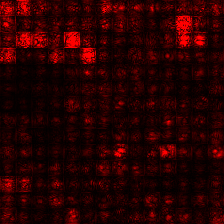
\includegraphics[width=0.085\textwidth]{figures/ptnb_v2/qualitative/butterfly/red_fox/gradient.png}
        & 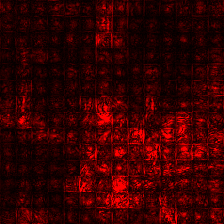
\includegraphics[width=0.085\textwidth]{figures/ptnb_v2/qualitative/butterfly/red_fox/smooth_grad.png}
        & 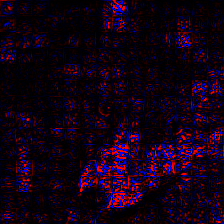
\includegraphics[width=0.085\textwidth]{figures/ptnb_v2/qualitative/butterfly/red_fox/integrated_gradients.png}
        & 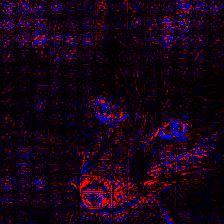
\includegraphics[width=0.085\textwidth]{figures/ptnb_v2/qualitative/butterfly/red_fox/dave.png}
        & 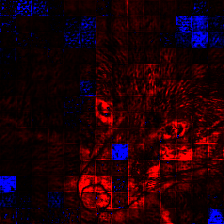
\includegraphics[width=0.085\textwidth]{figures/ptnb_v2/qualitative/butterfly/red_fox/lrp_gamma.png}
        & 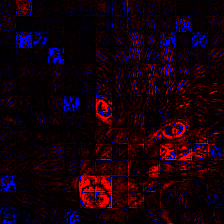
\includegraphics[width=0.085\textwidth]{figures/ptnb_v2/qualitative/butterfly/red_fox/attn_lrp.png}
        & 
\includegraphics[width=0.085\textwidth]{figures/ptnb_v2/qualitative/butterfly/red_fox/tibav.png} \\[1pt]
        \rotatebox{90}{\scriptsize\hspace{9pt}Kuvasz}
        & 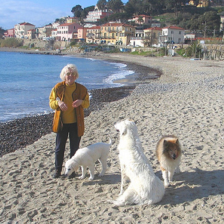
\includegraphics[width=0.085\textwidth]{figures/ptnb_v2/qualitative/butterfly/kuvasz/original.png}
        & 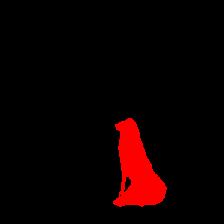
\includegraphics[width=0.085\textwidth]{figures/ptnb_v2/qualitative/butterfly/kuvasz/mask.png}
        & 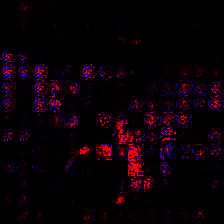
\includegraphics[width=0.085\textwidth]{figures/ptnb_v2/qualitative/butterfly/kuvasz/rg_loc.png}
        & 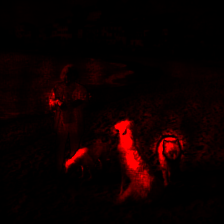
\includegraphics[width=0.085\textwidth]{figures/ptnb_v2/qualitative/butterfly/kuvasz/rgeq_loc.png}
        & 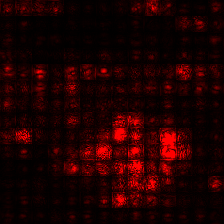
\includegraphics[width=0.085\textwidth]{figures/ptnb_v2/qualitative/butterfly/kuvasz/gradient.png}
        & 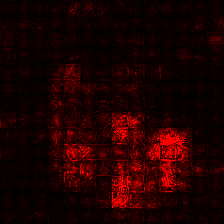
\includegraphics[width=0.085\textwidth]{figures/ptnb_v2/qualitative/butterfly/kuvasz/smooth_grad.png}
        & 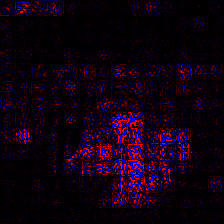
\includegraphics[width=0.085\textwidth]{figures/ptnb_v2/qualitative/butterfly/kuvasz/integrated_gradients.png}
        & 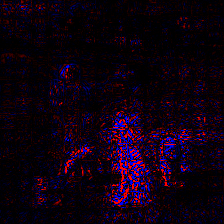
\includegraphics[width=0.085\textwidth]{figures/ptnb_v2/qualitative/butterfly/kuvasz/dave.png}
        & 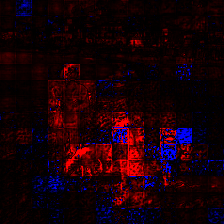
\includegraphics[width=0.085\textwidth]{figures/ptnb_v2/qualitative/butterfly/kuvasz/lrp_gamma.png}
        & 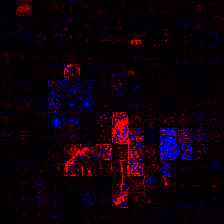
\includegraphics[width=0.085\textwidth]{figures/ptnb_v2/qualitative/butterfly/kuvasz/attn_lrp.png}
        & 
\includegraphics[width=0.085\textwidth]{figures/ptnb_v2/qualitative/butterfly/kuvasz/tibav.png} \\[1pt]
        \rotatebox{90}{\scriptsize\hspace{7pt}Wild boar}
        & 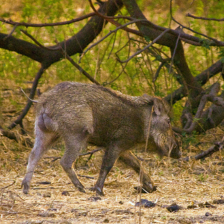
\includegraphics[width=0.085\textwidth]{figures/ptnb_v2/qualitative/butterfly/wild_boar/original.png}
        & 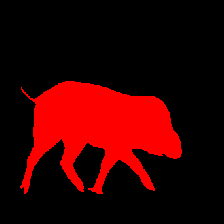
\includegraphics[width=0.085\textwidth]{figures/ptnb_v2/qualitative/butterfly/wild_boar/mask.png}
        & 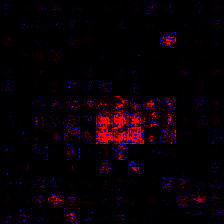
\includegraphics[width=0.085\textwidth]{figures/ptnb_v2/qualitative/butterfly/wild_boar/rg_loc.png}
        & 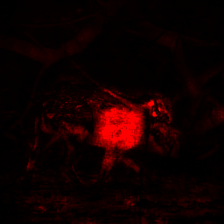
\includegraphics[width=0.085\textwidth]{figures/ptnb_v2/qualitative/butterfly/wild_boar/rgeq_loc.png}
        & 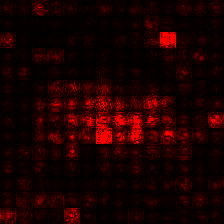
\includegraphics[width=0.085\textwidth]{figures/ptnb_v2/qualitative/butterfly/wild_boar/gradient.png}
        & 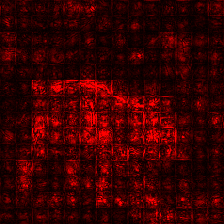
\includegraphics[width=0.085\textwidth]{figures/ptnb_v2/qualitative/butterfly/wild_boar/smooth_grad.png}
        & 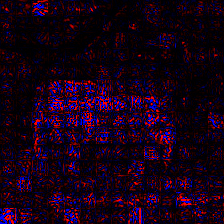
\includegraphics[width=0.085\textwidth]{figures/ptnb_v2/qualitative/butterfly/wild_boar/integrated_gradients.png}
        & 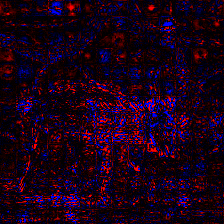
\includegraphics[width=0.085\textwidth]{figures/ptnb_v2/qualitative/butterfly/wild_boar/dave.png}
        & 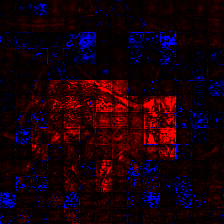
\includegraphics[width=0.085\textwidth]{figures/ptnb_v2/qualitative/butterfly/wild_boar/lrp_gamma.png}
        & 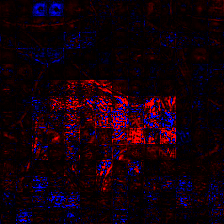
\includegraphics[width=0.085\textwidth]{figures/ptnb_v2/qualitative/butterfly/wild_boar/attn_lrp.png}
        & 
\includegraphics[width=0.085\textwidth]{figures/ptnb_v2/qualitative/butterfly/wild_boar/tibav.png} \\[1pt]
        \rotatebox{90}{\scriptsize\hspace{5pt}Black bear}
        & 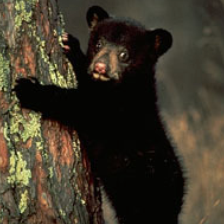
\includegraphics[width=0.085\textwidth]{figures/ptnb_v2/qualitative/butterfly/american_black_bear/original.png}
        & 
\includegraphics[width=0.085\textwidth]{figures/ptnb_v2/qualitative/butterfly/american_black_bear/mask.png}
        & 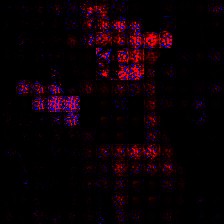
\includegraphics[width=0.085\textwidth]{figures/ptnb_v2/qualitative/butterfly/american_black_bear/rg_loc.png}
        & 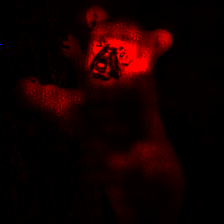
\includegraphics[width=0.085\textwidth]{figures/ptnb_v2/qualitative/butterfly/american_black_bear/rgeq_loc.png}
        & 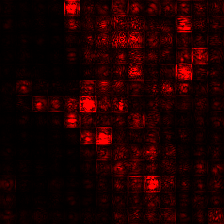
\includegraphics[width=0.085\textwidth]{figures/ptnb_v2/qualitative/butterfly/american_black_bear/gradient.png}
        & 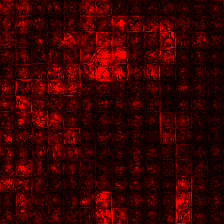
\includegraphics[width=0.085\textwidth]{figures/ptnb_v2/qualitative/butterfly/american_black_bear/smooth_grad.png}
        & 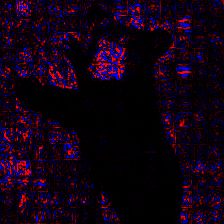
\includegraphics[width=0.085\textwidth]{figures/ptnb_v2/qualitative/butterfly/american_black_bear/integrated_gradients.png}
        & 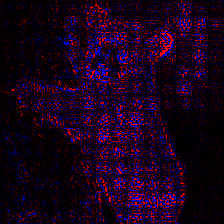
\includegraphics[width=0.085\textwidth]{figures/ptnb_v2/qualitative/butterfly/american_black_bear/dave.png}
        & 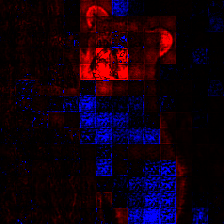
\includegraphics[width=0.085\textwidth]{figures/ptnb_v2/qualitative/butterfly/american_black_bear/lrp_gamma.png}
        & 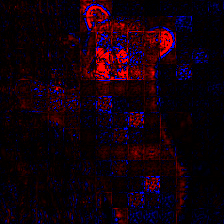
\includegraphics[width=0.085\textwidth]{figures/ptnb_v2/qualitative/butterfly/american_black_bear/attn_lrp.png}
        & 
\includegraphics[width=0.085\textwidth]{figures/ptnb_v2/qualitative/butterfly/american_black_bear/tibav.png} \\[1pt]
        \rotatebox{90}{\scriptsize\hspace{9pt}Airliner}
        & 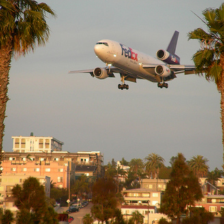
\includegraphics[width=0.085\textwidth]{figures/ptnb_v2/qualitative/butterfly/airliner/original.png}
        & 
\includegraphics[width=0.085\textwidth]{figures/ptnb_v2/qualitative/butterfly/airliner/mask.png}
        & 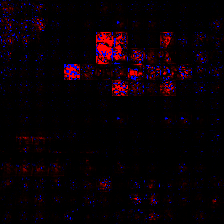
\includegraphics[width=0.085\textwidth]{figures/ptnb_v2/qualitative/butterfly/airliner/rg_loc.png}
        & 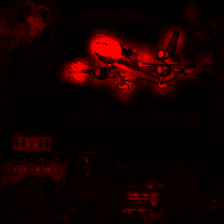
\includegraphics[width=0.085\textwidth]{figures/ptnb_v2/qualitative/butterfly/airliner/rgeq_loc.png}
        & 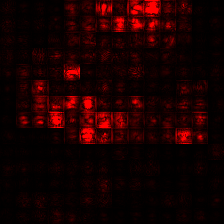
\includegraphics[width=0.085\textwidth]{figures/ptnb_v2/qualitative/butterfly/airliner/gradient.png}
        & 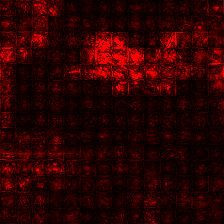
\includegraphics[width=0.085\textwidth]{figures/ptnb_v2/qualitative/butterfly/airliner/smooth_grad.png}
        & 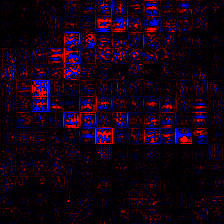
\includegraphics[width=0.085\textwidth]{figures/ptnb_v2/qualitative/butterfly/airliner/integrated_gradients.png}
        & 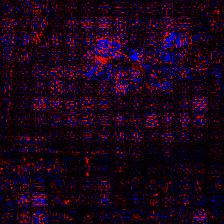
\includegraphics[width=0.085\textwidth]{figures/ptnb_v2/qualitative/butterfly/airliner/dave.png}
        & 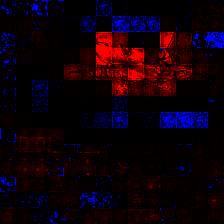
\includegraphics[width=0.085\textwidth]{figures/ptnb_v2/qualitative/butterfly/airliner/lrp_gamma.png}
        & 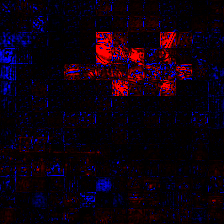
\includegraphics[width=0.085\textwidth]{figures/ptnb_v2/qualitative/butterfly/airliner/attn_lrp.png}
        & 
\includegraphics[width=0.085\textwidth]{figures/ptnb_v2/qualitative/butterfly/airliner/tibav.png} \\
    \end{tabular}
    }
    }%
\caption[ViT-B/16 qualitative comparison on six ImageNet-S examples]{Six ImageNet-S examples for ViT-B/16 at the localization-selected configurations of Table~\ref{ptnb:tab:eval-vit}; Gradient and TIBAV are fixed. Maps explain the dataset label, also the top-1 prediction except for the kuvasz (predicted: English setter). The first image is from the test split, the other five from validation. Red and blue show positive and negative attribution before the absolute-value reduction used for evaluation. Each sign is divided by its image-wide 99th percentile and clipped, saturating the top 1\%; all methods use this display transform. TIBAV is upsampled by nearest neighbor.}
    \label{fig:vit_saliency_comparison_main}
    \label{ptnb:fig:qualitative}
\end{figure}


\paragraph{ViT-B/16 (Table~\ref{ptnb:tab:eval-vit}).}
Figure~\ref{fig:vit_saliency_comparison_main} compares the selected methods on six images.
Under the localization-selected protocol, the \ac{rg} family beats every baseline on attribution
localization, including the prior transformer-specific backward methods
AttnLRP~\parencite{Achtibat2024AttnLRP}, our DAVE implementation~\parencite{Wrobel2024} (Section~\ref{ptnb:app:baselines}),
\ac{ptnbTIBAV}~\parencite{Chefer2021GenericAttention} and \ac{ptnbGAE}~\parencite{Chefer2021ICCV}: the selected mode
reaches AL \vitRGlocAL{} against \vitBestBaseAL{} for the best baseline (\vitBestBaseALname), and
\ac{rg}+Eq \vitRGEqlocAL{}, both significantly ahead of every baseline row after Holm correction.
\ac{rg}+Eq also has the highest observed TK (\vitRGEqlocTK{}), but the Holm-corrected tests do not detect a difference from \vitBestBaseTKname{}
at \vitBestBaseTK{} or LRP-$\gamma$ at $0.816$. The pointing game is led by \vitBestBasePGname{} (\vitBestBasePG{}), whose
maps are constant on superpixels: a hit needs only one pixel of the maximal region inside the mask.
Scoring a single pixel drawn from that region instead, KernelSHAP falls below \ac{rg}+Eq, which is
then not significantly below the best baseline (LRP-$\gamma$; Section~\ref{ptnb:app:pg-granularity}).
Among the localization-selected rows, faithfulness favors the \ac{lrp} rules: AttnLRP is best on PF$_5$ and PF$_{20}$ and LRP-$\gamma$ on
Sel (PF$_{20}$ \vitBestBasePFtwenty{} versus \vitRGlocPFtwenty{} for \ac{rg}), and the
faithfulness-selected \ac{rg} row narrows but does not close the gap (PF$_{20}$
\vitRGfaithPFtwenty{}). Across both selection objectives, faithfulness-selected AttnLRP has the lowest PF$_5$, PF$_{20}$ and Selectivity, at $7.64$, $6.12$ and $4.441$, respectively. The two anchors are the most robust rows (MaxS \vitRGanchorMaxS{} and
\vitRGEqanchorMaxS{} versus \vitBestBaseMaxS{} for \vitBestBaseMaxSname{}), with no Holm-significant MaxS difference between the two anchors. The
localization-selected mode reaches MaxS \vitRGlocMaxS{}: sharper routing trades robustness and
faithfulness for localization. \ac{ptnbADF} adds modest overhead (\ac{rg}: \vitRGlocTime\,s vs.\
\vitRGanchorTime\,s base), still below sampling baselines like SmoothGrad or IntGrad; Reynolds
averaging is the only expensive variant (\vitRGEqTime\,s), exceeding even the perturbation method
KernelSHAP (\vitSHAPTime\,s). We follow DAVE's transform-averaging strategy~\parencite{Wrobel2024} with 50 transformed inputs for \ac{rg}+Eq (Section~\ref{ptnb:app:equivariant}); we did not test smaller averaging counts. Detailed timings and their measurement scope are in Section~\ref{app:game_timing}.

\paragraph{Higher $\tau$ spreads attribution into context.}
The localization-optimal modes place mass on the few patches that align with the segmentation mask. As $\tau$ increases, routing spreads over more predecessors: the displayed examples retain object focus while extending attribution into context, without establishing which contextual features the model uses. Around the selected ViT-B/16 setting (Table~\ref{ptnb:tab:vit-temperature}), AL peaks at $0.723$ for $\tau{=}0.3$ and decreases to $0.461$ at $\tau{=}1$; lowering $\tau$ further to $0.2$ gives AL $0.699$ and PG $0.720$. Faithfulness is non-monotonic. High $\tau$ shows how localization scores favor concentrated maps within the same game. User-perceived informativeness remains untested.

% Localization-selected RG temperature sweep; values copied from the one-factor
% ViT-B/16 ablation in Appendix Table~\ref{ptnb:tab:ablations-vit}.
\begin{table}[tbp]
    \centering
    \caption[ViT-B/16 temperature sweep]{ViT-B/16 Routing Game temperature sweep on 565 ImageNet-S test images, with $\lambda_{\mathrm{sm}}=-10$, $\sigma^2=5$ and $\varepsilon=0.1$ fixed at the localization-selected settings (selected $\tau=0.4$). Metrics: Section~\ref{app:metrics}; full ablations: Table~\ref{ptnb:tab:ablations-vit}.}
    \label{ptnb:tab:vit-temperature}
    \TableContent{
        \small
        \setlength{\tabcolsep}{4pt}
        \renewcommand{\arraystretch}{0.92}
        \begin{tabular}{l*{9}{r}}
            \toprule
            $\tau$ & 1.0 & 0.9 & 0.8 & 0.7 & 0.6 & 0.5 & 0.4 & 0.3 & 0.2 \\
            \midrule
            AL$\uparrow$ & 0.461 & 0.477 & 0.506 & 0.556 & 0.632 & 0.691 & 0.711 & 0.723 & 0.699 \\
            PG$\uparrow$ & 0.628 & 0.683 & 0.743 & 0.777 & 0.827 & 0.830 & 0.825 & 0.816 & 0.720 \\
            PF$_5$$\downarrow$ & 8.36 & 8.29 & 8.22 & 8.16 & 8.16 & 8.23 & 8.27 & 8.33 & 8.36 \\
            PF$_{20}$$\downarrow$ & 7.42 & 7.28 & 7.13 & 6.97 & 7.00 & 7.31 & 7.48 & 7.64 & 7.71 \\
            \bottomrule
        \end{tabular}
    }%
\end{table}

\begin{figure}[htbp]
    \QualitativeImageContent{
    \centering
    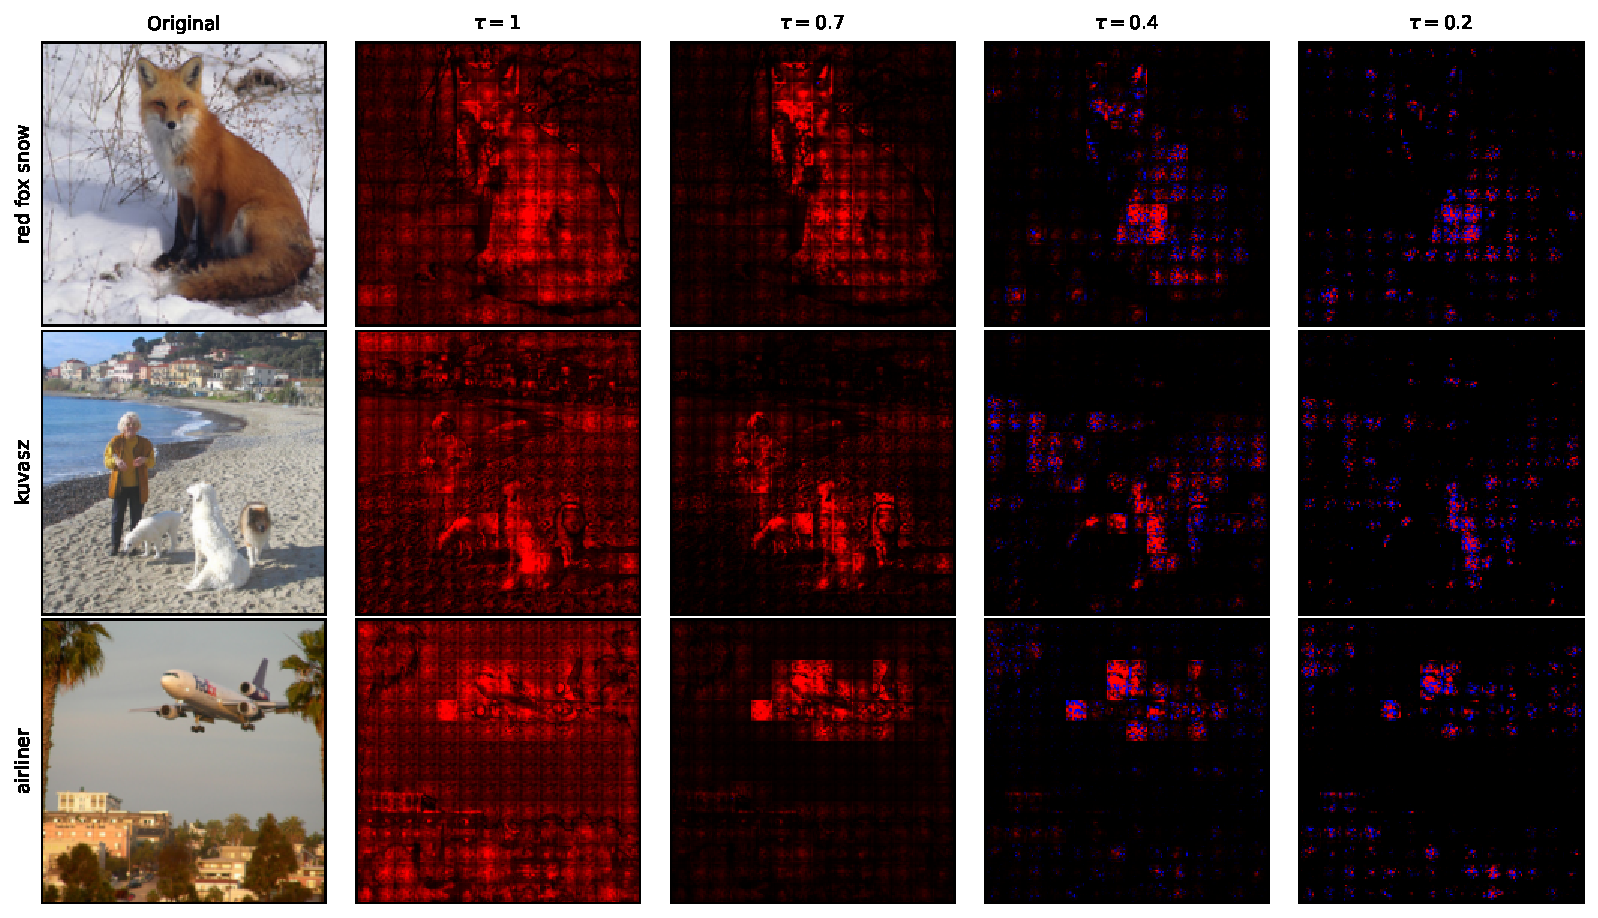
\includegraphics[width=\textwidth]{figures/rg_temperature/rg_temperature_sweep.pdf}
    }
    \caption[Qualitative effect of routing temperature for ViT-B/16]{Temperature controls how strongly backward routing favors larger contributions: in these examples, lowering $\tau$ turns broad heatmaps into sparser maps concentrated on fewer image regions. Routing Game maps on three ImageNet-S examples are shown at $\tau=1,0.7,0.4,0.2$, from left to right. The red fox is from the test split; the kuvasz and airliner are from the validation split. All panels use the same ViT-B/16 checkpoint, target labels, and RG settings ($\alpha=2$, $\beta=1$, $\varepsilon=0.1$, $\lambda_{\mathrm{sm}}=-10$, input variance $5$, merged attention--Value rule); only $\tau$ varies. Each sign is scaled by the image-wise 99th percentile and clipped, with positive relevance in red and negative relevance in blue.}
    \label{fig:vit_temperature}
\end{figure}


\begin{table}[htbp]
    \centering
    \caption[ViT-B/16 Routing Game attention rule ablation]{\ac{vit}-B/16, \ac{rg}: attention ablation on 565 ImageNet-S test images at the anchor and validation-selected settings. Cells: gradient fallback above; composite Value rule (Theorem~\ref{ptnb:thm:attn-ab-recovery}, gray) below. Configurations: Section~\ref{ptnb:app:config-symbols}. $^{\dagger}$: paired bootstrap (McNemar for PG), Holm-corrected over the table, $p<0.05$.}
    \label{ptnb:tab:abl-gradient-fallback}
\TableContent{
    \setlength{\tabcolsep}{2pt}
    \renewcommand{\arraystretch}{0.9}
    \small
    \appfitgen{tables/ptnb_v2/generated/attention_rule_vit_b16_tabular}
}%
\end{table}

\paragraph{Cross-dataset transfer (Pascal VOC).}
A natural worry with validation-tuned modes is that the chosen $\tau$, $\lambda_{\mathrm{sm}}$ and
$\sigma^2$ are overfitted to the ImageNet-S 50-class subset. We test transfer on a per-image
disjoint split of Pascal VOC 2012 trainval ($2{,}743$ test (image, foreground-class) samples with
pixel-accurate segmentation masks): \ac{rg} and \ac{rg}+Eq use the \emph{same} mode parameters as
Table~\ref{ptnb:tab:eval-vit} without any VOC-side re-tuning, while every baseline gets a fresh
per-method validation grid on the new pool. This tests the portability of the selected parameters
across these datasets for the same pretrained model, without identifying whether the underlying
structure is model-specific or dataset-specific. The localization lead carries over (AL
\vocRGlocAL{} for \ac{rg} and \vocRGEqlocAL{} for \ac{rg}+Eq versus \vocBestBaseAL{} for
\vocBestBaseALname{}, both significant against every baseline row), while TK and PG are led by
\ac{ptnbTIBAV} and the perturbation methods, and faithfulness by the \ac{lrp} rules
(Section~\ref{ptnb:app:voc-cross-data}).

\paragraph{VGG-16 and ResNet-50 (Section~\ref{ptnb:app:results}).}
On the CNNs, where \ac{lrp}-type rules are already strong, the localization-selected \ac{rg} rows also lead on AL within that selection: clearly on VGG-16 (\vggRGlocAL{} versus \vggBestBaseAL{} for \vggBestBaseALname{}) and narrowly on ResNet-50 (\resRGlocAL{} versus \resBestBaseAL{} for \resBestBaseALname{}). The ResNet-50 difference is not Holm-significant (adjusted $p=0.420$), so its numerical lead does not establish superiority. Across both objectives, VGG-16's strongest baseline AL is faithfulness-selected LRP-$\varepsilon$ at $0.639$, below \ac{rg}'s \vggRGlocAL{}. Pixel Flipping favors LRP-$\varepsilon$ for VGG-16 PF$_5$ ($12.43$), LRP-$\gamma$ for VGG-16 PF$_{20}$ ($7.89$ versus LRP-$\varepsilon$'s $8.17$), and LRP-$\gamma$ for both ResNet-50 metrics; \ac{cam} and perturbation methods lead TK and PG. On VGG-16 the risk-averse \ac{sg} mode is the most robust method (MaxS \vggSGlocMaxS{} versus \vggBestBaseMaxS{} for \vggBestBaseMaxSname{}).

\subsection{Game-Method Ablations}\label{subsec:mode_ablation}

One-factor mode ablations around validation-selected configurations (Section~\ref{ptnb:app:abl-one-factor}; 565 test images), granularity-controlled Pointing Game (Section~\ref{ptnb:app:pg-granularity}), and attention-rule comparisons (Table~\ref{ptnb:tab:abl-gradient-fallback}) expose trade-offs among localization, perturbation faithfulness and robustness. These diagnostics do not affect selection.

\paragraph{Gradient-fallback attention.}\label{ptnb:app:abl-gradient-fallback}

The \ac{rg} backward holds the realized attention policy fixed and routes relevance only through the Value path, with zero gradient on $Q$, $K$, as in CP-LRP~\parencite{Ali2022AttnLRP} (Section~\ref{ptnb:app:vit-implementation}). Gradient fallback uses pure autograd through attention, recovering zennit-style $\varepsilon$-\ac{lrp}; Value-routing risk $\lambda_\text{sm}$ is inactive. Fallback lowers all three localization metrics in every configuration (AL and TK significantly throughout) and worsens every PF$_5$, PF$_{20}$ and Sel cell, significantly in four of nine.

\subsection{Additional Experimental Controls}\label{sec:additional-controls}

\paragraph{Separating map concentration from feature ranking.}
Power sharpening replaces a spatial attribution map $a$ by $(|a|/\max|a|)^p$. With $p=1.5$, large scores become more dominant relative to small scores. This can increase AL, which measures the fraction of attribution mass inside the object mask. The pixel order is unchanged, so Pixel Flipping removes the same features in the same order and PF$_{20}$ stays unchanged. Table~\ref{tab:sharpening-control} gives both powers for all four methods in this control. Sharpened AttnLRP reaches AL $0.7153$, close to unsharpened RG's $0.7112$, with PF$_{20}$ $6.1226$ versus $7.4807$; its lower PF$_{20}$ is already present before sharpening. Applying the same sharpening to RG raises its AL to $0.7807$. Appendix~\ref{app:rebuttal-sharpening} gives the validation-matching protocol and paired intervals.

\begin{table}[htbp]
\centering
\TableContent{
\small
\begin{tabular}{lrrr}
\toprule
Method & AL, $p=1$ & AL, $p=1.5$ & PF$_{20}$ (unchanged) $\downarrow$ \\
\midrule
LRP-$\gamma$ & 0.6138 & 0.6942 & 6.3977 \\
AttnLRP & 0.6291 & 0.7153 & 6.1226 \\
RG anchor & 0.5093 & 0.5550 & 6.9673 \\
RG (loc) & 0.7112 & 0.7807 & 7.4807 \\
\bottomrule
\end{tabular}

}
\caption[Effect of fixed power sharpening on ViT-B/16 attribution maps]{Effect of fixed power sharpening on ViT-B/16 attribution maps, evaluated on the same 565 test images. LRP-$\gamma$ and AttnLRP use the configurations selected by validation AL proximity to the localization-selected RG row at $p=1.5$, held fixed at both powers; RG anchor and RG (loc) use their anchor and localization-selected configurations. The transform is $(|a|/\max|a|)^p$. PF$_{20}$ is unchanged within each method because its feature ranking is preserved; lower is better.}
\label{tab:sharpening-control}
\label{tab:rebuttal-common-power}
\end{table}


\paragraph{Deleting and restoring complete pixels.}
A second faithfulness control removes or restores all three color channels of each pixel together and follows the model score over the entire image, rather than only the initial deletion fraction. Across target-logit and target-probability scores, LRP baselines outperform RG in both deletion and insertion. Table~\ref{tab:rebuttal-full-auc} reports all seven configurations and their confidence intervals.

\paragraph{Isolating the effect of risk aversion.}
On all 565 ViT test images, the validation-selected risk setting reduces Maximum Sensitivity from $0.6850$ to $0.6013$, while AL decreases from $0.6706$ to $0.5204$. For VGG-16, we hold the activation-gating rule fixed to distinguish the risk term's effect from gate smoothing: Maximum Sensitivity falls from $0.5265$ to $0.4865$, with AL changing from $0.6207$ to $0.6107$. Table~\ref{tab:rebuttal-risk} separates the effects of smoothing, risk aversion, and their combination.

% VIT_EXTENSION_INSERT_HERE
% BEGIN VIT_EXTENSION_GENERATED
\appneedspace{12\baselineskip}
\section{Transformer DC Extension Results}
\label{sec:vit-extension}

Hidden Monotonicity develops SplitCAM for ReLU networks and CNNs, leaving the DC decomposition of Transformers open~\parencite{hiddenMono}. The following experiments are new to this thesis and test whether the GELU split and stabilized Transformer implementation extend SplitCAM's CNN gains to ViTs (Sections~\ref{sec:closed_form_dc_activations} and~\ref{sec:transformer_dc}). We compare SplitCAM with Grad-CAM and LayerCAM, tuning them on the game benchmark's 50 validation images and evaluating on its 565 test images with the same ViT-B/16 and metrics.

\begin{center}
    \captionsetup{hypcap=false}
    \captionof{table}[ViT-B/16: extension results with confidence intervals]{ViT-B/16 extension results on the same ImageNet-S test split (565 images; MaxS/AvgS: the fixed 200-image subset), with 95\% image-bootstrap confidence intervals. Gradient is copied from Table~\ref{ptnb:tab:test-ci-vit}; the other configurations were selected on the same 50 validation images. Labels loc/faith denote the unchanged selection criteria. Bold/dark shading marks the best row; $^{\approx}$/light shading marks no significant difference under Holm adjustment across all row pairs within each metric of this table (Section~\ref{ptnb:app:stats}).}
    \label{tab:vit-extension}
\end{center}
\captionsetup{hypcap=true}
\appinputgenci{tables/vit_extension/generated/extension_ci_longtable}
\noindent $B$ is the one-based block index (LN1 readout). SplitCAM uses the signed paper formulas without ReLU; $F$, $L$ and $U$ denote fixed attention and LayerNorm, fixed LayerNorm only, and both live. Configurations with $p$ use adaptive common-component scaling and the selected backward scale power; the remaining SplitCAM rows use the paper post-shifts. Fixed quantities are recomputed for each perturbed input. CAM baselines retain their library normalization and bilinear resize; SplitCAM retains signed maps and nearest-neighbor resize. All metrics apply their original absolute-value preprocessing. This exploratory comparison evaluates complete pipelines, including their different map normalization and resizing, so it does not isolate the DC decomposition's effect. Gradient pairwise tests use archived rounded per-image scores; its original confidence intervals are retained. Three test illustrations were viewed during method development.
The paper-postshift search admitted no validation configuration for $L$, $U$.

\paragraph{Performance and comparison with the game methods.}
With fixed attention and LayerNorm, localization-selected SplitCAM at block 11 achieves the highest localization means in Table~\ref{tab:vit-extension}: AL $0.614$, PG $0.827$ and TK $0.741$, compared with LayerCAM's $0.603$, $0.758$ and $0.714$ and Grad-CAM's $0.500$, $0.596$ and $0.563$. It also lowers Maximum Sensitivity to $0.620$, versus LayerCAM's $0.828$. LayerCAM retains better Pixel Flipping scores (PF$_{20}$ $7.73$ versus $7.96$). The faithfulness-selected block-6 SplitCAM configuration performs worse on the test faithfulness metrics than the block-11 configuration.

On these same test images, localization-selected RG and RG+Eq achieve higher AL ($0.711$ and $0.698$) and lower PF$_{20}$ ($7.48$ and $7.80$) than SplitCAM (Table~\ref{ptnb:tab:eval-vit}). SplitCAM's PG $0.827$ is close to RG's $0.825$; its Maximum Sensitivity $0.620$ is lower than RG's $0.729$, but higher than RG+Eq's $0.441$. Thus the Transformer extension improves CAM localization, while the game methods retain the stronger AL--Pixel Flipping results. These cross-table comparisons concern the reported means; the extension table's significance markers cover only its own rows.

% END VIT_EXTENSION_GENERATED

\section{Experimental Conclusions}\label{sec:experimental_conclusions}

The two papers demonstrate complementary benefits of structural attribution. The DC decomposition improves localization and Selectivity through SplitCAM, while SplitLRP achieves the lowest Maximum Sensitivity in the VGG-16 comparison, without retraining the underlying model. The game framework turns changes of routing into strong ViT localization methods: RG and RG+Eq lead the original localization-selected comparison, and their lead transfers to Pascal VOC without retuning. The controls explain these gains more precisely: map concentration, feature ranking, and robustness measure different properties. Together with the verified gradient and relevance identities and the trajectory diagnostics, these results establish a mathematical and empirical basis for understanding, deriving, and improving backward attribution methods.
